% Selectionne le format du papier, la taille de police d'écriture, le modèle du document.
\documentclass[a4paper,11pt]{article}

%%%%%%%%%%%%%%%%%%%%%%%%%%%%%%%%%%%%%%%%%%%%%%%%%%%%%%%%%%%%%%%%%%%%%%%%%%%%%%%%%%%%%%%%

% Document en français, anglais, allemand, ou italien. 
\usepackage[french,english,german,italian]{babel}
% Evite le problème des accents.
\usepackage[utf8]{inputenc}
% Permet d'incorporer des images.
\usepackage{graphicx}
% Permet de la flexbilité sur la géométrie,
\usepackage{geometry}
% Package pour les maths.
\usepackage{amsfonts,amsmath,amsthm,amssymb,amsfonts}
% Package pour dessiner des tableaux.
\usepackage{array}
% csquotes va utiliser la langue définie dans babel.
\usepackage[babel=true]{csquotes}
% Pour inserer des liens,
% hyperindex ajoute des liens dans les index,
% colorlinks autorise de colorier les liens,
% linkcolor selectionne la couleur des liens interne,
% urlcolor selectionne la couleur des hyperliens.
\usepackage[hyperindex=true,colorlinks=true,linkcolor=black,urlcolor=black]{hyperref}
% Permet d'utiliser des couleurs personnalisées (black, white, red, green, blue, cyan, magenta).
\usepackage{color}
% Permet de barrer ces éléments.
\usepackage{cancel}
% Permet de faire correspondre une légende à plusieurs figures.
\usepackage{subfigure}
% Permet de mettre une partie de son document sur plusieurs colonnes.
\usepackage{multicol}
% Permet d'inserer d'autres symboles mathématique.
\usepackage{latexsym}
% Iseere une nouvelle font.
\usepackage{pifont}
% Permet de créer une autre table des matières avec une profondeur différente.
\usepackage{shorttoc}

%%%%%%%%%%%%%%%%%%%%%%%%%%%%%%%%%%%%%%%%%%%%%%%%%%%%%%%%%%%%%%%%%%%%%%%%%%%%%%%%%%%%%%%%

% Il y a trois styles de base pour \theoremstyle :
%    \theoremstyle{plain} pour les théorèmes, lemmes, corollaires, conjectures,
%    \theoremstyle{definition} pour les  définitions, exemples, problèmes,
%    \theoremstyle{remark} pour les remarques, notes, conclusions.

% Structure de la commande :
%          \newtheorem{nico}{Nicolas} :
%                 - nico est la commande à utiliser dans le code latex,
%                 - Nicolas est ce qui va s'afficher.
%          \newtheorem{nico}{Nicolas}[niveau] :
%                 - nico est la commande à utiliser dans le code latex,
%                 - Nicolas est ce qui va s'afficher,
%                 - Nicolas sera numéroté en fonction de niveau (section, subsection, ...).
%          \newtheorem{nico}[Papa]{Nicolas} :
%                 - nico est la commande à utiliser dans le code latex,
%                 - Nicolas est ce qui va s'afficher,
%                 - Nicolas sera numéroté en fonction des niveau Papa.


\theoremstyle{plain}
\newtheorem{thm}{Théorème}[section]
\newtheorem{cor}{corollaire}[section]
\newtheorem{lem}{Lemme}[section]

\theoremstyle{definition}
\newtheorem{dfn}{Définition}[section]
\newtheorem{conj}{Conjecture}[section]
\newtheorem{hpts}{Hypothèse}[section]
\newtheorem{prop}[dfn]{Propriété}
\newtheorem{ex}[dfn]{Exemple}
\newtheorem{demo}[thm]{Preuve}

\theoremstyle{remark}
\newtheorem{rem}{Remark}[section]
\newtheorem{note}{Note}
\newtheorem{case}{Case}

%%%%%%%%%%%%%%%%%%%%%%%%%%%%%%%%%%%%%%%%%%%%%%%%%%%%%%%%%%%%%%%%%%%%%%%%%%%%%%%%%%%%%%%%

% Permet de numéroter des éléments suivant la/les section(s) où ils se trouvent.
\numberwithin{equation}{section}
\numberwithin{equation}{subsection}
\numberwithin{figure}{section}

%%%%%%%%%%%%%%%%%%%%%%%%%%%%%%%%%%%%%%%%%%%%%%%%%%%%%%%%%%%%%%%%%%%%%%%%%%%%%%%%%%%%%%%%

% Titre.
\title{Renormalisation des théories de Jauge}
% Auteur
\author{
\href{mailto:gereantoine@gmail.com}{Antoine Géré}
\footnote{
\href{http://marwww.in2p3.fr/Master_M2_P3TMA_Physique_Theorique_et_Mathematique_Physique_des_Particules_et_Astrophysique/
}{Université d'Aix Marseille, Master 2 Physique Théorique et Mathématique, Physique des Particules et Astroparticules}
}}

%%%%%%%%%%%%%%%%%%%%%%%%%%%%%%%%%%%%%%%%%%%%%%%%%%%%%%%%%%%%%%%%%%%%%%%%%%%%%%%%%%%%%%%%

\begin{document}


\selectlanguage{french}


\maketitle


\begin{abstract}

Du 13 mars au 11 juin 2012, j'ai effectué mon stage de master 2, au laboratoire de physique théorique d'Orsay, sous la direction de Jean-Christophe Wallet. Mon travail a été centré sur la renormalisation des théories de Yang-Mills, depuis la pratique du calcul de diagrammes de Feynman, jusqu’à la construction récursive des contre-termes via les identités de Slavnov liés à la symétrie BRST de l’action fixée de jauge. Je me suis également intéréssé à la construction de théorie des champs sur des espaces non-commutatifs. Afin de manipuler ces objets ''non commutatifs'' j'ai réalisé quelques calculs de corrections radiatives dans des théories de jauge construites sur certains espaces non commutatifs, déformations de $\mathbb{R}^2$ et $\mathbb{R}^4$, ce afin de regarder des limites infrarouges  intéressantes en 2-D. Si certains de ces calculs sont déjà disponibles dans la littérature, d’autres relatifs à des théories de jauge plus difficiles à manoeuvrer restaient à faire.\\

En plus de présenter mon travail de stage, j'ai voulu par ce rapport établir une synthése de ce que j'avais compris en théories des champs. Certains developpements sont donc issus de mon apprentissage des cours de cette année de master 2. Je n'ai malheuresement pas eu la place d'inserer l'étude de l'electrodynamique.  J'ai par contre fait un rappel en annexe concernant l'obtention des règles de Feynman. J'ai écris ce rapport avec la volonté qu'il soit accésible avec le moins de prerequis possible.\\

En parallèle de cet aspect théories des champs, j'ai commencé à travaillé sur des questions de distances sur la sphere de Podles. Mais ceci ne fait pas l'objet de develloppement dans ce present rapport, du fait que ce sujet déborde tres clairement du cadre fixée au départ, qui était les théories de jauge.

\end{abstract}


\begin{figure}[b]
\begin{center}

\includegraphics[scale=0.4]{logoRapport.jpg}
\end{center}
\end{figure}


\newpage


\tableofcontents 

%%%%%%%%%%%%%%%%%%%%%%%%%%%%%%%%%%%%%%%%%%%%%%%%%%%%%%%%%%%%%%%%%%%%%%%%%%%%%%%%%%%%%%%%%%%%%%%%%%%%%%%%%%%%%%%%%%%%%%%%%%%%%%%%%%
\section{Introduction}
%%%%%%%%%%%%%%%%%%%%%%%%%%%%%%%%%%%%%%%%%%%%%%%%%%%%%%%%%%%%%%%%%%%%%%%%%%%%%%%%%%%%%%%%%%%%%%%%%%%%%%%%%%%%%%%%%%%%%%%%%%%%%%%%%%

Avant 1970, la comprehension de la physique des particules élémentaires comportait de nombreuses zones d'ombres. Bien que de nombreux succès de la théories des champs aient été observé et reconnu, l'opinion majoritaire était que la théorie des champs n'était pas la bonne voie pour aboutir un jour à une bonne compréhension des ces phénomènes physique. En effet la présence de ces fameux ''infini'' dans la théorie laissait présager qu'elle ne pourait pas donner entiere satisfaction. Le devellopement perturbatif n'était pas encore accepté, et selon beaucoup de physisien était la source de ces problèmes. Il semblait nécessaire de reformuler la théorie, de sorte que ces ''infinis'' disparaissent. Une étape importante a été franchi losqu'en 1947 H. Bethe trouva une expression satisfaisante pour le decalage de Lamb. Par la suite J. Schwinger parvint à calculer la premiere correction quantique de maniere sytématique. S.I. Tomonaga et R. Feynman, à la vue de ces travaux, établirent les premières bases du ménanisme de renormalisation. De nombreux autres physiciens apportèrent des contributions essentielles au développement de cette théorie de la renomalisation. Mentionnons quelques un de ces physiciens, F. Dyson, J. Ward, A. Salam, et S. Weinberg, pour ne citer qu'eux. \\

En 1954 C.N. Yang et R.L. Mills publièrent un article dans lequel ils généralisèrent le concept de théorie de jauge, jusque là connu pour l'electrodynamqiue, théorie de jauge abélienne, à une théorie non abélienne. L'objectif de cette généralisation était d'expliquer l'intéraction forte. Cette idée a été critiqué par W. Pauli, car pour conserver l'invariance de jauge, la théories est sans masse. Il s'avera plus tard que l'idée de C.N. Yang et R.L. Mills était correcte, les termes de masses étant obtenue par brisure de symétrie. Cette notion de brisure de symétrie ne sera pas étudiée dans ce rapport.\\

Ces théories de jauge sont à la base de nombreuses théories physiques. L'électro-dynamique, l'électrofaible, la QCD sont des théories de jauge. Il est interessant de noter que même la théorie de la gravitation, c'est à dire la relativité générale d'Einstein, est une théorie de jauge. Les quatres intéractions fondamentales peuvent donc être comprise dans le cadre des théories de jauge. \\

Mentionnons quelques dates marquantes dans l'histoire de la construction de la théorie de Yang-Mills.
\begin{description}
 \item[1954] Yang et Mills proposent une théorie de jauge non abélienne. Ils généralisent, l'invariance de jauge connu pour QED, à l'interaction faible et l'invariance de l'isospin.
 \item[1967] Faddeev, Popov, et de Witt proposent une métode de quantificationdu champ de Yang Mills sams termes de masse. La même année Weinbeg et Salam proposent une théorie de jauge qui unifie QED et l'intéraction faible.
 \item[1971] G. 't Hooft montre que la méthode de quantification des théorie de Yang et Mills sans masses peut être étendu au cas d'une brisure spontanée de symétrie.
\end{description}

De nombreuses contributions ont permis de construire une théorie quantique des champs de jauge dans le cadre de la théorie des perturbations. La preuve de la renormalisabilabitité de cette théorie a été faite via les identité de Slavnov, qui sont les identites de Ward généralisée, issu de la symétrie ''cachée'' de Becchi, Rouet, Stora, et Tyupkin (BRST). \\

%%%%%%%%%%%%%%%%%%%%%%%%%%%%%%%%%%%%%%%%%%%%%%%%%%%%%%%%%%%%%%%%%%%%%%%%%%%%%%%%%%%%%%%%%%%%%%%%%%%%%%%%%%%%%%%%%%%%%%%%%%%%%%%%%%
 \section{Quelques considérations classiques}
%%%%%%%%%%%%%%%%%%%%%%%%%%%%%%%%%%%%%%%%%%%%%%%%%%%%%%%%%%%%%%%%%%%%%%%%%%%%%%%%%%%%%%%%%%%%%%%%%%%%%%%%%%%%%%%%%%%%%%%%%%%%%%%%%%

\noindent
Nous allons nous interesser ici aux théories de jauge. Une théorie de jauge est une théorie des champs pour laquelle le lagrangien est invariant sous des transformations dites de jauge.\\
Nous travaillerons avec un groupe de Lie compact semi simple de dimension $n$, noté $G$, et avec une algèbre de Lie dénoté $\cal{G}$. $G$ et $\cal{G}$ seront représenté via la représentation adjointe, noté $adj$. Une matrice $A$ de $adj(\cal{G})$ pourra s'écrire comme une combinaison linéaire de $n$ générateurs. 
\begin{eqnarray}
 A = T^{a} \alpha^{a}, \hspace{2mm} \text{avec} \hspace{1mm} a =(1,...,n).
\end{eqnarray}
On choisit une normalsation des générateurs de $adj(\cal{G})$ de façon à avoir :
\begin{eqnarray}
 tr( T^{a} T^{b} ) &=& -2 \delta^{ab} ,  \\
 \left [ T^{a} ,  T^{b} \right] &=& f^{abc} T^{c} ,
\end{eqnarray}
où $f^{abc}$ est la constante de structure de $\cal{G}$, completement antisymétrique.

%%%%%%%%%%%%%%%%%%%%%%%%%%%%%%%%%%%%%%%%%%%%%%%%%%%%%%%%%%%%%%%%%%%%%%%%%%%%%%%%%%%%%%%%%%%%%%%%%%%%%%%%%%%%%%%%%%%%%%%%%%%%%%%%%%
\subsection{Analyse géométrqiue}
%%%%%%%%%%%%%%%%%%%%%%%%%%%%%%%%%%%%%%%%%%%%%%%%%%%%%%%%%%%%%%%%%%%%%%%%%%%%%%%%%%%%%%%%%%%%%%%%%%%%%%%%%%%%%%%%%%%%%%%%%%%%%%%%%%

\noindent
On se donne un fibré principal $P(M,G)$, où $M$ est la variété considéré et $G$ le groupe de structure.\\
On note $V_{p}$ l'ensemble des vecteurs tangents à $p$ en un point p du fibré.
\begin{eqnarray}
 V_{p} = \left \{  \frac{d}{dt} \left( p\hspace{0.5mm} e^{tX} \right)_{|t=0} / X \in \cal{G}  \right \}
\end{eqnarray}
Ils forment l'ensemble des vecteurs verticaux. Il n'y a pas de notion naturelle de vecteurs horizontaux. Ces '' vecteurs horizontaux'' 
sont les vecteurs tangent à la variété $M$, que l'on remonte dans le fibré. On note cet ensemble $H_{p}$. On dira qu'une forme differentielle 
$\omega_{|p}$ est horizontale si, évalué sur un vecteur vertical, elle s'annule : $\omega_ {|p} (x^{v}_{|p}) = 0$. De même $\omega_{|p}$ sera 
dite verticale si elle s'annule lorsqu'on l'évalue sur un vecteur horizontal.\\
Nous pouvons à présent définir ce qu'est une 1-forme de connexion. On définit une 1-forme de connexion $\omega_{|p}$ sur P à valeur dans 
$\cal{G}$, en posant, pour tout $p \in P$,
\begin{itemize}
 \item $\omega_{|p} (X_{|p}) = 0$ pour tout $X_{|p} \in H_{p}$
 \item $\omega_{|p} (X_{|p}) = A$ pour tout $X_{|p} \in V_{p}$ .
\end{itemize}
On peut associer à cette 1-forme de connexion, une 2-forme de courbure sur P, en posant $\Omega = D \omega$, où $D$ est la differentielle covariante. 
Cette 2-forme $\Omega$ verifie l'équation de structure de cartan :
\begin{eqnarray}
 \Omega (X,Y) = d_{p} \omega (X,Y) + \frac{1}{2} \left [ \omega (X) , \omega (Y) \right ].
\end{eqnarray}
avec $d_{p}$ la différentielle exterieure sur $P$. \\
On peut montrer que $\Omega$ verifie l'équation de Bianchi :
\begin{eqnarray}
 D \Omega = 0 = d_{p} \Omega (X,Y) +  \left [ \omega  , \Omega  \right ].
\end{eqnarray}
Une notion importante est celle de groupe de jauge. On appelle groupe de jauge du fibré P, l'ensemble de ses automorphismes verticaux. 
Un automorphisme $\Phi$ est vertical sur le fibré P, si les trois conditions suivantes sont vérifiées :
\begin{itemize}
 \renewcommand{\labelitemi}{$\bullet$}
 \item 1. $\Phi$ est un difféomorphisme de P.
 \item 2. La fibre $\pi^{-1} (x)$ au dessus de x est stable par $\phi$.
 \item 3. $\forall p \in P, \forall g \in G , \Phi (pg) = \Phi(p) g$
\end{itemize}
On montre qu'il est équivalent de caractériser un groupe de jauge des trois façons suivante :
\begin{itemize}
 \renewcommand{\labelitemi}{$\bullet$}
 \item 1. L'ensemble des automoprhismes vertiacaux $ f: P \to P$.
 \item 2. L'ensemble des application ($\psi : P \to G$) differentiable G-equivariante pour l'application de G dans G, défini comme $a \to g a g^{-1}$.
 \item 3. L'ensemble des sections différentiable $S : M \to P \times G$.
\end{itemize}

\noindent
Maintenant ce que l'on souhaiterait, c'est ''ramener'' $\omega$ et $\Omega$ sur la variété M. Pour cela, il faut définir ce qu'on apelle une 
trivialisation locale $(U_{i}, \Phi)$, de section trivialisante $s: U_{i} \rightarrow \pi^{-1} (U_{i})$, où $s(x) = \Phi (x,e)$. \\
On peut descendre localement la 1-forme de connexion sur P, sur l'ouvert $U_{i}$, en posant :
\begin{eqnarray}
 A{i} = s_{i}*\omega
\end{eqnarray}
qui est une 1-forme sur $U_{i}$ à valeur dans $\cal{G}$.
De la même façon on a :
\begin{eqnarray}
 F_{i} = s_{i}*\Omega
\end{eqnarray}
où F est une 2-forme sur u à valeur dans $\cal{G}$. \\
Sur $U_{i} \cap U_{j}$ A et F, precedement defini, se recollent de la façon suivante $(U_{i}$ à 
un ouvert $U_{j}$ ($U_{i} \cap U_{j} \ne \emptyset )$ :
\begin{eqnarray}
 A_{j} &=& g^{-1}_{ij} A_{i} g_{ij} + g^{-1}_{ij} d g_{ij} \\
 F_{j} &=& g^{-1}_{ij} F_{i} g_{ij} 
\end{eqnarray}
où $g_{ij} : U_{i} \cap U_{j}  \to  G$.\\
Si l'on revient à la physique, A représente le champ de jauge. Les formules de recollement sont en fait les transformations de jauge. De plus 
l'équation de structure de Cartan nous donne :
\begin{eqnarray}
 F_{\mu \nu} &=&  \partial_{\nu}A_{\mu} - \partial_{\mu}A_{\nu} + [A_{\mu},A_{\nu}]
\end{eqnarray}

%%%%%%%%%%%%%%%%%%%%%%%%%%%%%%%%%%%%%%%%%%%%%%%%%%%%%%%%%%%%%%%%%%%%%%%%%%%%%%%%%%%%%%%%%%%%%%%%%%%%%%%%%%%%%%%%%%%%%%%%%%%%%%%%%%
\subsection{Équation du mouvement, et autres}
%%%%%%%%%%%%%%%%%%%%%%%%%%%%%%%%%%%%%%%%%%%%%%%%%%%%%%%%%%%%%%%%%%%%%%%%%%%%%%%%%%%%%%%%%%%%%%%%%%%%%%%%%%%%%%%%%%%%%%%%%%%%%%%%%%

\noindent
On considere des champs $A_{\mu}$ à valeurs dans $\cal{G}$. Par analogie avec l'electrodynamique, on parvient à écrire le lagrangien 
de la théorie de Yang Mills. Nous rappelons que le lagrangien de l'electrodynmqiue s'écrit comme : $\mathcal{L}_{\small EL} = F_{\mu\nu}F_{\mu \nu}$ 
où, $F_{EL \hspace{1mm} \mu \nu}= \partial_{\nu}A_{\mu} - \partial_{\mu}A_{\nu}$. On ecrit donc dans le cas des théorie de Yang Mills,
\begin{eqnarray}
\mathcal{L}_{\small YM} = \frac{1}{8} tr\left(F_{\mu\nu}F_{\mu \nu}\right)
\end{eqnarray}
où,
\begin{eqnarray}
F_{\mu \nu}=\partial_{\nu}A_{\mu} - \partial_{\mu}A_{\nu} + g[A_{\mu},A_{\nu}].
\end{eqnarray}
La densité lagrangienne s'écrit alors comme :
\begin{eqnarray}
\mathcal{L}_{\small YM} = \frac{-1}{4} F^{a}_{\mu\nu}F^{a}_{\mu \nu},
\end{eqnarray}
où
\begin{eqnarray}
F^{a}_{\mu \nu}=\partial_{\nu}A^{a}_{\mu} - \partial_{\mu}A^{a}_{\nu} + gf^{abd}A^{b}_{\mu}A^{d}_{\nu}.
\end{eqnarray}
En apliquant le principe variationnel de la théorie des champs classique, on parvient à écrire les équations du mouvement.
\begin{eqnarray}
 \delta \cal{I}_{YM}  &=&  \frac{1}{8}  \int  Tr\left(\delta ( F_{\mu \nu} ) F_{\mu \nu} \right) dx \\
                                    &=&  \frac{1}{8}  \int  Tr\left(\delta A_{\nu} ( D_{\mu} F_{\mu \nu} )  \right) dx
\end{eqnarray}
où $D_{\mu}$ est la dérivée covariante, $D_{\mu} \bullet  =  \partial_{\mu} \bullet  + g [ A_{\mu} , \bullet ] $.
Les équations du mouvement sont donc :
\begin{eqnarray}
D_{\mu} F_{\mu \nu} &=&  0.
\end{eqnarray}
Il est possible de réécrire le lagrangien, en distinguant partie temporelle et partie spatiale sur les indice, tel que : 
$\mu = (0,k)$ , $\nu = (0,l)$ , où $(k,l) = (1, 2, 3)$. Une première astuce est d'écrire $\mathcal{L}_{\small YM}$ comme :
\begin{equation}
 \mathcal{L}_{\small YM} = \frac{1}{4} tr\left[ \left( \partial_{\nu}A_{\mu} - \partial_{\mu}A_{\nu} + g[A_{\mu},A_{\nu}] 
+ F_{\mu\nu} \right)F_{\mu \nu}\right].
\end{equation}
Ensuite si l'on considére $A_{\mu}$ et $F_{\mu \nu}$ comme des variables indépendantes, c'est à dire sans développer $F_{\mu \nu}$, 
et en effectuant une intégration par partie, on arrive à écrire :
\begin{eqnarray}
\mathcal{L}_{\small YM} = \frac{-1}{2} tr\left( E_{k}(\partial_{0} A_{k}) - \frac{1}{2}(E_{k}^{2} + B_{k}^2) + A_{0}C\right)
\end{eqnarray}
où,
\begin{eqnarray}
 E_k &=& F_{k0}\\
 B_k &=& \frac{1}{2} \epsilon_{ijk} F_{ij}\\
 C &=& \partial_{k} E_{k} - g[A_k , E_k] 
\end{eqnarray}
On peut identifier $E_k$ et $B_k$ comme respectivement le champ électrique et le champ magnétique de la théorie de Yang Mills. Il est 
interessant de remarquer qu'à partir des équations du mouvement, on peut écrire deux équations qui sont en fait des équations de Maxwell 
pour la théorie de Yang Mills.
\begin{eqnarray}
 D_{k}  F^{a}_{k0}  &=& 0   \\
 D_{\mu} F^{a}_{\mu k} &=& 0.
\end{eqnarray}
En deloppant ces deux relations on obtient :
\begin{eqnarray}
 \partial_{k} E^{a}_{k}  + g f^{abd} A^{b}_{k} E^{d}_{k}  &=& 0,  \\
 \partial_{0} E^{a}_{k} + 2 \epsilon_{lik} \partial_{i} B^{a}_{l} + g f^{abd} A^{b}_{0} E^{d}_{k } 
+ 2 g  f^{abd} A^{b}_{i} \epsilon_{lik} B^{d}_{l } &=& 0,
\end{eqnarray}
qui sont deux ''pseudos équations de Maxwell'' pour la théorie de Yang Mills.
 
\noindent
Comme nous l'avons vu dans la partie précédente la transformation de jauge, s'écrit de la façon suivante :
\begin{eqnarray}
 A_{\mu} \rightarrow  A^{\omega}_{\mu}(x)=\omega(x)A_{\mu}(x)\omega^{-1}(x) + ( \partial_{\mu} \omega(x) ) \omega^{-1}(x)
\end{eqnarray}
Il est facile de montrer que $F_{\mu \nu}$ se transforme comme $g F_{\mu \nu} g^{-1}$. On en déduit de suite que le lagrangien de Yang Mills est invariant sous cette transformation. \\


%%%%%%%%%%%%%%%%%%%%%%%%%%%%%%%%%%%%%%%%%%%%%%%%%%%%%%%%%%%%%%%%%%%%%%%%%%%%%%%%%%%%%%%%%%%%%%%%%%%%%%%%%%%%%%%%%%%%%%%%%%%%%%%%%%
 \section{Quantification du champ de Yang Mills}
%%%%%%%%%%%%%%%%%%%%%%%%%%%%%%%%%%%%%%%%%%%%%%%%%%%%%%%%%%%%%%%%%%%%%%%%%%%%%%%%%%%%%%%%%%%%%%%%%%%%%%%%%%%%%%%%%%%%%%%%%%%%%%%%%%



%%%%%%%%%%%%%%%%%%%%%%%%%%%%%%%%%%%%%%%%%%%%%%%%%%%%%%%%%%%%%%%%%%%%%%%%%%%%%%%%%%%%%%%%%%%%%%%%%%%%%%%%%%%%%%%%%%%%%%%%%%%%%%%%%%
\subsection{Intoduction à l'intégrale de chemin}
%%%%%%%%%%%%%%%%%%%%%%%%%%%%%%%%%%%%%%%%%%%%%%%%%%%%%%%%%%%%%%%%%%%%%%%%%%%%%%%%%%%%%%%%%%%%%%%%%%%%%%%%%%%%%%%%%%%%%%%%%%%%%%%%%%

\noindent
Nous savons qu'un système à un degré de liberté est régit par l'équation de Shrödinger,
\begin{eqnarray}
 i \hbar \partial_{t'} \psi(x,t') &=& \textbf{H} \psi(x,t')
\end{eqnarray}
où $\textbf{H}$ est l'hamiltonien du système.
L'évolution temporelle de $\psi(x,t)$, entre les instants $t'$ et $t''$, est représenté par l'opérateur d'évolution $\textbf{U(t,t')}$,
\begin{eqnarray}
 \psi (x,t') &=& \textbf{U}(t',t'') \psi (x,t'')
\end{eqnarray}
où $U(t',t'')$ vérifie :
\begin{eqnarray}
  i \hbar \partial_{t'}  \textbf{U}(t',t'') &=& \textbf{H}  \textbf{U}(t',t'')
\end{eqnarray}
La solution de cette équation est :
\begin{eqnarray}
  \textbf{U}(t',t'') &=& exp \left( \frac{t'-t''}{i \hbar}  \textbf{H} \right).
\end{eqnarray}
En se plaçant dans le système d'unité naturel, où $\hbar=1$, on a :
\begin{eqnarray}
  \textbf{U}(t',t'') &=& exp \left( i (t'-t'') \textbf{H} \right).
\end{eqnarray}
Notre but va être d'écrire la matrice $\mathcal{S}$ par la méthode de l'intégrale de chemin pour l'oscillateur harmonique. 
La matrice $\mathcal{S}$ est en fait l'opérateur d'évolution $ \textbf{U}(t',t'') $  entre les temps $t'' \rightarrow - \infty$ 
et $t' \rightarrow - \infty$ . \\
La densité hamiltonienne pour l'oscillateur hamiltonienne s'écrit comme :
\begin{equation}
 h(p,q) = \frac{p^{2}}{2} + \frac{\omega^{2}q^{2}}{2}
\end{equation}
On introduit les amplitudes complexes suivantes :
\begin{eqnarray}
 a = \frac{1}{\sqrt{2 \omega}} \left( \omega q + i p \right)  \hspace{1cm}  &&  
\hspace{1cm} q =  \frac{1}{\sqrt{2 \omega}} \left( a + a^{\star} \right)\\
&\Longleftrightarrow&  \\
 a^{\star} = \frac{1}{\sqrt{2 \omega}} \left( \omega q - i p \right)   \hspace{1cm}  &&  
\hspace{1cm} q = i \sqrt{\frac{\omega}{2}} \left( a^{\star} - a \right)\\
\end{eqnarray}
où $a^{\star}$ désigne le conjugué de $a$.
La densité se réécrit donc comme suit :
\begin{equation}
 h = \omega a^{\star} a
\end{equation}
On a dans cette représentation le produit saclaire suivant :
\begin{equation}
 \langle f_{1} | f_{2} = \rangle \int \left(f_{1} (a^{\star})\right)^{\star} f_{2} (a^{\star}) e^{- a^{\star} a } \frac{da^{\star} da}{2i \pi}
\end{equation}
Une fonction analytique arbitraire $f (a^{\star})$ peut s'écrire comme une combinaison linéaire de monômes (développement en série de Laurent),
\begin{equation}
 \psi_{n} = \frac{(a^{\star})^n}{\sqrt{n !}}
\end{equation}
On montre facilement que : 
\begin{equation}
 \langle \psi_{n} | \psi_{m} \rangle = \delta_{nm}.
\end{equation}\\

\noindent
Soit \textbf{A} un opérateur arbitarire. On peut écrire :\\
\begin{equation}
 (\textbf{A}f)(a^{\star}) = \int A(a^\star,\alpha) f(\alpha^{\star}) e^{-\alpha^{\star} \alpha } \frac{d\alpha^{\star} d\alpha}{2i \pi}
\end{equation}
avec $ A(a^\star,a) $  le noyau de \textbf{A}. Le noyau s'écrit de la façon suivante :
\begin{eqnarray}
 A(a^{\star},a) &=& \sum_{n,m} A_{n,m} \frac{ (a^{\star})^{n} }{ \sqrt{n !} } \frac{a^{m}}{\sqrt{m!}}\\
                &=&  \sum_{n,m} A_{n,m} \psi_{n} \psi_{m}
\end{eqnarray}
où,
\begin{equation}
 A_{n,m} = \langle \psi_{n} | \textbf{A} | \psi_{m} \rangle
\end{equation}

\noindent
Les opérateur qui vont nous préocuper ici sont l'opérateur hamiltonien $\textbf{H}$, et l'opérateur d'évolution $\textbf{U}$. On 
note $\textbf{U}$, l'opérateur d'évolution pour l'intervalle de temps $\Delta t$ supposé petit. On a donc :
\begin{eqnarray}
 \textbf{U}(\Delta t) &=& exp( -i \textbf{H} \Delta t )\\
             &=& 1 - i \textbf{H} \Delta t
\end{eqnarray}
le noyau de $\textbf{U}(\Delta t)$ est :
\begin{eqnarray}
 U(a^{\star} , a, \Delta t) &=& \sum_{n,m} \langle \psi_{n} | \textbf{U}(\Delta t) | \psi_{m} \rangle  \psi_{n} \psi_{m}^{\star}
\end{eqnarray}
où,
\begin{eqnarray}
 \langle \psi_{n} | U(\Delta t) | \psi_{m} \rangle &=& \langle \psi_{n} | 1 - i \textbf{H} \Delta t | \psi_{m} \rangle \\
                                                   &=& \langle \psi_{n} | \psi_{m} \rangle \left( 1 - i h(a^{\star},a) \Delta t \right) \\
                                                   &=& \delta_{nm} \left( 1 - i h(a^{\star},a) \Delta t \right) \\
                                                   &=&  \delta_{nm} e^{-i h (a^{\star},a) \Delta t}
\end{eqnarray}
donc, 
\begin{eqnarray}
 U(a^{\star} , a, \Delta t) &=& \sum_{n, m} \delta_{nm} e^{-i h (a^{\star},a) \Delta t} \psi_{n} \psi_{m}^{\star} \\
                            &=& \sum_{n} e^{-i h (a^{\star},a) \Delta t} \frac{\left(a a^{\star}\right)^{n}}{n !}\\
 U(a^{\star} , a, \Delta t) &=& exp\left(a a^{\star} - i h(a , a^{\star}) \Delta t \right) 
\end{eqnarray}
Dans le cas général on a un intervalle de temps $(t''-t')$, qui n'est pas forcé d'être petit, bien au contrairre. Pour pouvoir 
utiliser la même méthode que dans le cas d'un  intervalle $\Delta t$ petit, c'est à dire pour pouvoir dévelloper l'exponentielle, 
on écrit $ (t''-t') = N \frac{(t''-t')}{N} = N \Delta t$, avec $N \rightarrow \infty$, c'est à dire $\Delta t \rightarrow 0$. On a alors :
\begin{equation}
  U(a^{\star} , a, t''-t') = \int exp \left( a(t'') a^{\star}(t'') 
+ \int_{t'}^{t''} dt \left[ -a^{\star} \dot{a} - i h(a^{\star},a) \right] \right) \frac{da^{\star} da}{2i \pi}
\end{equation}
ce que l'on peut réécrire, en effectuant une intégration par partie, comme :
\begin{eqnarray}
 U(a^{\star} , a, t''-t') &=& \int exp \left(  \frac{1}{2} \left( a(t'') a^{\star}(t'') + a(t') a^{\star}(t') \right)  \right. \nonumber \\
&& \left. + i \int_{t'}^{t''} dt \left( \frac{1}{2i} \left(\dot{a}^{\star}a - a^{\star} \dot{a} \right) - i h(a^{\star},a) \right) \right) 
\frac{da^{\star} da}{2i \pi}
\end{eqnarray}
À présent que nous avons déterminer $U(a^{\star} , a, t''-t') $, nous sommes en mesure d'obtenir l'expression de la matrice  $\mathcal{S}$. Afin d'obtenir son expression on écrit : 
\begin{eqnarray}
 \mathcal{S} = \lim_{t'' \to + \infty \atop t' \to - \infty} U(a^{\star} , a, t''-t')
\end{eqnarray}
Pour finaliser notre description de $\mathcal{S}$ étudions comportement asymptotique des deux amplitudes complexes. Les équations d'Euler-Lagrange nous permettent d'écrire :
\begin{eqnarray}
 &&\dot{a}^{\star}(t) - i \omega a^{\star}(t) = 0 \\
 &&\dot{a}(t) - i \omega a(t) = 0 
\end{eqnarray}
On a comme condition limite, $a^{\star}(t'') = a^{\star}$, et $a(t')=a$.\\
On a alors :
\begin{eqnarray}
 &&a^{\star}(t) = a^{\star} e^{ i \omega (t - t') }\\
 &&a(t) = a e^{ i \omega (t'' - t) }
\end{eqnarray}
L'expression finale de la matrice $\mathcal{S}$ est donc :
\begin{equation}
 \mathcal{S} = \int exp \left(  \frac{1}{2} \left( a a^{\star} + a a^{\star} \right)  
+ i \int_{-\infty}^{+ \infty} dt \left[ \frac{1}{2i} \left(\dot{a}^{\star}a - a^{\star} \dot{a} \right) - i h(a^{\star},a) \right] \right) 
\frac{da^{\star} da}{2i \pi}
\end{equation}

%%%%%%%%%%%%%%%%%%%%%%%%%%%%%%%%%%%%%%%%%%%%%%%%%%%%%%%%%%%%%%%%%%%%%%%%%%%%%%%%%%%%%%%%%%%%%%%%%%%%%%%%%%%%%%%%%%%%%%%%%%%%%%%%%%
\subsection{Quantification hamiltonienne}
%%%%%%%%%%%%%%%%%%%%%%%%%%%%%%%%%%%%%%%%%%%%%%%%%%%%%%%%%%%%%%%%%%%%%%%%%%%%%%%%%%%%%%%%%%%%%%%%%%%%%%%%%%%%%%%%%%%%%%%%%%%%%%%%%%



%%%%%%%%%%%%%%%%%%%%%%%%%%%%%%%%%%%%%%%%%%%%%%%%%%%%%%%%%%%%%%%%%%%%%%%%%%%%%%%%%%%%%%%%%%%%%%%%%%%%%%%%%%%%%%%%%%%%%%%%%%%%%%%%%%
\subsubsection{Mise en évidence de la dynamique hamiltonienne}
%%%%%%%%%%%%%%%%%%%%%%%%%%%%%%%%%%%%%%%%%%%%%%%%%%%%%%%%%%%%%%%%%%%%%%%%%%%%%%%%%%%%%%%%%%%%%%%%%%%%%%%%%%%%%%%%%%%%%%%%%%%%%%%%%%

\noindent
Soit $\omega(x)$ une matrice à valeur dans $\cal{G}$.\\
Nous définissons la transformation de jauge comme suit :
\begin{center}
$A_{\mu} \rightarrow  A^{\omega}_{\mu}(x)=\omega(x)A_{\mu}(x)\omega^{-1}(x) + ( \partial_{\mu} \omega(x) ) \omega^{-1}(x)$
\end{center}
Le lagrangien de Yang-Mills, invariant sous cette transformation de Jauge, s'écrit de cette manière : 
\begin{eqnarray}
\mathcal{L}_{\small YM} = \frac{1}{8} tr\left(F_{\mu\nu}F_{\mu \nu}\right),
\end{eqnarray}
\begin{eqnarray}
\text{où} \hspace{2mm} F_{\mu \nu}=\partial_{\nu}A_{\mu} - \partial_{\mu}A_{\nu} + g[A_{\mu},A_{\nu}].
\end{eqnarray}
Ce que l'on peut réécrire comme l'on sait de cette façon :
\begin{eqnarray}
\mathcal{L}_{\small YM} = \frac{-1}{2g} tr\left( E_{k}(\partial_{0} A_{k}) - \frac{1}{2}(E_{k}^{2} + B_{k}^2) + A_{0}C\right)
\end{eqnarray}
où, 
\begin{eqnarray}
 E_k &=& F_{k0}\\
 B_k &=& \frac{1}{2} \epsilon_{ijk} F_{ij}\\
   C &=& \partial_{k} E_{k} - g[A_k , E_k] 
\end{eqnarray}
On a alors,
\begin{eqnarray}
 \mathcal{L}_{\small YM} &=& E_{k}^{a}(\partial_{0} A_{k}^{a}) - h(E_{k}^{a},A_{k}^{a}) + A_{0}^{a}C\\
 \text{où, \hspace{1cm}} h(E_{k}^{a},A_{k}^{a}) &=& \frac{1}{2}\left[(E_{k}^{a})^{2} + (B_{k}^{a})^2 \right]
\end{eqnarray}
On peut noter que le lagrangien correspondant au système libre est le suivant :
\begin{equation}
 \mathcal{L}_{0} = E_{k}^{a}(\partial_{0} A_{k}^{a}) - h(E_{k}^{a},A_{k}^{a}).
\end{equation}
Si on regarde la théorie de yang Mills comme un syteme mecanique classique, en appliquant le formalisme lagrangien, 
on voit que $E_{k}$ et $A_{k}$ sont les coordonnées canoniquement conjuguées l'une de l'autre, avec le crochet de poisson suivant :
\begin{eqnarray}
  \{ E_{k}^{a}(x) , A_{l}^{b}(y) \} = \delta^{ab} \delta_{kl} \delta(x-y).
\end{eqnarray}
On dit que le lagrangien est écrit en fonction des variables canonique $A_{k}^{a}=q$ et $E_{k}^{a}=p$. 
La composante temporelle $A_{0}$ n'a pas de variable conjuguée, elle sert de multiplicateur de lagrange afin d'imposer la contrainte $C=0$. 
On calcul assez facilement le crochet de poisson de la contrainte :
\begin{eqnarray}
 \{ c^{a}(x) , c^{b}(y) \} = g c^{d}(x) f^{abd} \delta(x-y).
\end{eqnarray}
On note que l'hamiltonien du système s'écit comme :
\begin{eqnarray}
 h(E_{k}^{a},A_{k}^{a}) &=& \frac{1}{2}\left[(E_{k}^{a})^{2} + (B_{k}^{a})^2 \right],
\end{eqnarray}
qui est invariant de jauge, et dont le crochet de poisson avec la contrainte est nul.
\begin{eqnarray}
 \{ H , c^{b} \} = 0 
\end{eqnarray}
Ceci nous donne une information interessante, en effet la contrainte sera une constante de la dynamique de notre système.

%%%%%%%%%%%%%%%%%%%%%%%%%%%%%%%%%%%%%%%%%%%%%%%%%%%%%%%%%%%%%%%%%%%%%%%%%%%%%%%%%%%%%%%%%%%%%%%%%%%%%%%%%%%%%%%%%%%%%%%%%%%%%%%%%%
\subsubsection{Jauge de Coulomb}
%%%%%%%%%%%%%%%%%%%%%%%%%%%%%%%%%%%%%%%%%%%%%%%%%%%%%%%%%%%%%%%%%%%%%%%%%%%%%%%%%%%%%%%%%%%%%%%%%%%%%%%%%%%%%%%%%%%%%%%%%%%%%%%%%%

\noindent
Les coordonnées canonique $q$ et $p$ précedement identifiées définissent un espaces des phases. Mais les trajectoires dans cette 
espace des phaes dépendent du multiplicateur de lagrange $A^{a}_{0}$. Or on souhaiterais que celle-ci n'en dépende pas. 
Pour ce faire on doit imposer autant de contraintes supplementaires que le système n'en possedent déja. 
Or il n'y a qu'une seule contrainte. Il nous faut donc imposer une seule conditions supplementaires afin de définir 
l'espace des phases réduit, où les trajectoires ne dépendraient plus du multiplicateur de Lagrange $A^{a}_{0}$. On choisi donc comme 
contraintes supplémentaire, la jauge de Coulomb.
\begin{equation}
 \partial_{k} A_{k} := 0.
\end{equation}
qui vérifie bien :
\begin{eqnarray}
 \left \{  \partial_{k} A_{k} , \partial_{k} A_{k} \right \} = 0
\end{eqnarray}
Il est necessaire d'avoir,
\begin{eqnarray}
 det \left \{ C,  \partial_{k} A_{k}  \right \}  \ne  0
\end{eqnarray}
Or on a,
\begin{eqnarray}
  \left \{ C^{a}(x) , \partial_{k} A^{b}_{k} (y) \right \} &=& \partial_{k} \left [ \partial_{k} \delta^{ab} - g f^{abd} A_{k}^{d} \right ] \delta(x-y)  \\
                                                             &=&   M_{c} \delta(x-y).
\end{eqnarray}
Il est possible de montrer que $M_{c}$ s'exprime sous forme d'une série en $g$. Par analogie avec l'electrodynamique on écrit :
\begin{eqnarray}
 A_{k}  &=&   A_{k}^{L}  +   A_{k}^{T}  \\
 E_{k}  &=&   E_{k}^{L}  +  E_{k}^{T}  
\end{eqnarray}
où 
\begin{eqnarray}
 \partial_{k}  A_{k}^{T}  = 0  =  \partial_{k}  E_{k}^{T}
\end{eqnarray}
et,
\begin{eqnarray}
 A_{k}^{L}   &=&  \partial_{k}  B(x)  \hspace{2cm}  B(x) = \frac{1}{4 \pi}  \int \frac{1}{|x-y|}  \partial_{k}  A_{k}  (y)  dy       \\
 E_{k}^{L} &=& \partial_{k}  Q
\end{eqnarray}
L'equation des contraintes s'écrit comme :
\begin{eqnarray}
 C E_{k} = 0 & \Leftrightarrow & \Delta Q - g[A_k , \partial_k Q ] - g[ A_k , E^{T}_{k}  ]  =  0  \\
             & \Leftrightarrow & M_{c} Q =  g[ A_k , E^{T}_{k} ]  \\
             & \Leftrightarrow & Q =  g M_{c}^{-1} [ A_k , E^{T}_{k} ]
\end{eqnarray}
On obtient $Q$ comme une série en g, fonction de $A^{T}_{k}$ et $E_{k}^{T}$. En injectant ceci dans l'expression de l'hamiltonien de départ $h$, 
on arrive à exprimer $h^{\star}$, hamiltonien de l'espace des phases réduit, comme une série en g.
On a en plus comme coordonnées canonique de notre nouvel espace des phase, 
\begin{eqnarray}
 && p^{\star} = E_{k}^{T} \\
 && q^{\star} = A_{k}^{T}.
\end{eqnarray}
Il faut noter que $E_{k}^{T}$ et $A_{k}^{T}$ ont deux états de polarisations.
Les variables canoniques de notre nouvel espace des phase s'expriment en fonction des amplitudes complexes suivantes, introduites dans la 
représentations holomorphes :
\begin{eqnarray}
 &&a^{\star}_{i}(k,t)\\
 &&a_{i}(k,t)
\end{eqnarray}

\noindent
Par analogie avec le cas simple de l'oscillateur harmonqiue, on écrit  :
\begin{eqnarray}
 A^{T,b}_{l} (x,t) &=& \left( \frac{1}{2 \pi} \right)  \int \frac{ d^{3}k }{ \sqrt{2 \omega} } 
\sum_{i=1,2} \left(  a^{\star^{b}}_{i}(k,t) u^{i}_{l}(-k) e^{-ikx}  +   a^{b}_{i}(k,t) u^{i}_{l}(k) e^{-ikx}  \right)\\
 E^{T,b}_{l} (x,t) &=& \left( \frac{1}{2 \pi} \right)  \int d^{3}k 
\sum_{i=1,2} \left(  a^{\star^{b}}_{i}(k,t) u^{i}_{l}(-k) e^{-ikx}  -   a^{b}_{i}(k,t) u^{i}_{l}(k) e^{-ikx}  \right) 
\left(i \sqrt{\frac{\omega}{2}} \right) \nonumber \\
\end{eqnarray}
Par commodité pour la suite nous posons,
\begin{eqnarray}
 \alpha &=& a^{\star^{b}}_{i}(k,t) u^{i}_{l}(-k) e^{-ikx}  +   a^{b}_{i}(k,t) u^{i}_{l}(k) e^{-ikx}\\
 \epsilon &=& a^{\star^{b}}_{i}(k,t) u^{i}_{l}(-k) e^{-ikx}  -   a^{b}_{i}(k,t) u^{i}_{l}(k) e^{-ikx}
\end{eqnarray}

\noindent
On a aussi :
\begin{eqnarray}
 \mathcal{S} &=& \lim_{t'' \to + \infty \atop t' \to - \infty}
\int exp \left( 
i \int d^{3}k \sum_{i=1,2} \left[ a^{\star^{b}}_{i}(k,t'') a^{b}_{i}(k,t'') + a^{\star^{b}}_{i}(k,t') a^{b}_{i}(k,t') \right] \right. \nonumber \\ 
&& + \left. i \int^{t''}_{t'} dt \int d^{3}k 
\sum_{i=1,2} \left[ \dot{a}^{\star^{b}}_{i}(k,t) a^{b}_{i}(k,t) + a^{\star^{b}}_{i}(k,t) \dot{a}^{b}_{i}(k,t) - h^{\star} \right]
\right) \frac{da^{\star} da}{2i \pi}. \nonumber  \\
\end{eqnarray}
Si on fait le petit calcul suivant :
\begin{equation}
 \epsilon \dot{\alpha} - \dot{\epsilon} \alpha = 2 \left(\dot{a}^{\star^{b}}_{i}(k,t) a^{b}_{i}(k,t) 
+ a^{\star^{b}}_{i}(k,t) \dot{a}^{b}_{i}(k,t) \right),
\end{equation}
on voit de suite que l'on peut écrire :
\begin{eqnarray}
 \mathcal{S} &=& \lim_{t'' \to + \infty \atop t' \to - \infty}
\int exp \left( 
i \int d^{3}k \sum_{i=1,2} \left[ a^{\star^{b}}_{i}(k,t'') a^{b}_{i}(k,t'') + a^{\star^{b}}_{i}(k,t') a^{b}_{i}(k,t') \right] \right. \nonumber  \\ 
&& + \left. i \int^{t''}_{t'} dt \int d^{3}k 
\sum_{i=1,2} \left[ \frac{-1}{4} tr\left(E^{T}_{l} \dot{A}^{T}_{l} - \dot{E}^{T}_{l} A^{T}_{l} \right)  - h^{\star} \right]
\right) \frac{da^{\star} da}{2i \pi}
\end{eqnarray}

\noindent
On a la matrice $\cal{S}$ donc normalement on a tout ! Mais $h^{\star}$, qui est notre nouvel hamiltonien (fonction de $E^{T}_{k}$ et $A^{T}_{k}$) 
sur l'espace des phases réduit, n'est connu que sous la forme d'une série en $g$ ! De plus on integre sur tout les $x$, ceci pose un problème car 
on a considéré au départ une jauge locale !\\

\noindent
\underline{Solutions à nos problèmes} :\\
\begin{itemize}
 \item On va intégrer sur tout les $A_{\mu}$ et $E_{k}$ de sorte à ''récupérer'' le lagrangien de départ.
 \item Pour se restreindre quand même à notre espace des phases réduit, on insere $\delta \left( \partial_{k} A_{k} \right)$ qui va permetre 
de selectionner seulement les champs d'une seule classe de jauge, c'est à dire un ensemble de $A_{\mu}$ indépendant.
 \item On introduira $det(M_{c})$ qui jouera le rôle du jacobien pour la condition de jauge (ceci est expliqué plus en détail dans la partie concernant
la méthode de Faddeev Popov).
\end{itemize}

\noindent
La matrice $\cal{S}$ peut donc s'écrire comme :
\begin{eqnarray}
 \mathcal{S} &=& \lim_{t'' \to + \infty \atop t' \to - \infty}
\int exp \left( 
i \int d^{3}k \sum_{i=1,2} \left[ a^{\star^{b}}_{i}(k,t'') a^{b}_{i}(k,t'') + a^{\star^{b}}_{i}(k,t') a^{b}_{i}(k,t') \right] \right. \nonumber \\ 
&& + \left. i \int^{t''}_{t'} dt \int d^{3}k 
\left[ \frac{-1}{4} tr\left(E_{l} \dot{A}_{l} - \dot{E}_{l} A_{l} \right) E^{2}_{l} - B^{2}_{l} 
+ 2 \left( \partial_{l} E_{l} - g [A_{l} , E_{l} ] \right) \right]
\right) \nonumber \\
&& \delta( \partial_{l}A_{l} ) det(M_{c}) dA_{l} dE_{l} dA_{0}
\end{eqnarray} 
Que l'on peut encore écrire comme :
\begin{eqnarray}
 \mathcal{S} &=& N^{-1} \int exp \left( 
i \int dx \frac{1}{8} tr \left( F_{\mu\nu} F_{\mu\nu} \right) \right) 
\delta( \partial_{l}A_{l} ) det(M_{c}) dA_{\mu}
\end{eqnarray} 
 
\noindent
On a malgré tout toujours un problème très génant, on a une matrice $\cal{S}$  qui n'est manifestement pas covariante. On est tenté de prolonger 
ce que l'on vient de faire pour la jauge de Lorentz $\partial_{\mu} A_{\mu}=0$, qui est covariante par définition. Pour faire ceci on va utiliser 
la méthode de Faddeev Popov.

%%%%%%%%%%%%%%%%%%%%%%%%%%%%%%%%%%%%%%%%%%%%%%%%%%%%%%%%%%%%%%%%%%%%%%%%%%%%%%%%%%%%%%%%%%%%%%%%%%%%%%%%%%%%%%%%%%%%%%%%%%%%%%%%%%
\subsubsection{Méthode de Faddeev Popov}
%%%%%%%%%%%%%%%%%%%%%%%%%%%%%%%%%%%%%%%%%%%%%%%%%%%%%%%%%%%%%%%%%%%%%%%%%%%%%%%%%%%%%%%%%%%%%%%%%%%%%%%%%%%%%%%%%%%%%%%%%%%%%%%%%%

\noindent
L'idée tres astucieuse de Faddeev et Popov est de bien réécrie  1, en terme d'une fonctionnelle invariante de jauge et d'une intégrale sur 
le parametre de jauge.\\
Débutons par un exemple simple afin de se familiariser avec cette méthode. \\

\noindent
\textit{\underline{Un exemple à deux dimensions}}\\

\noindent
On considere une action $\mathcal{I}_{2D}$ invariante par rotation dans un espace à deux dimensions. La matrice $\mathcal{S}_{2D}$ s'écrit comme :
\begin{eqnarray}
 \mathcal{S}_{2D} &=& \int \mathcal{D}(r,\theta) exp\left(i\mathcal{I}_{2D}(r,\theta)\right) 
\end{eqnarray}
L'idée est d'écrire $1$ de la bonne façon ! Faddeev et Popov ont réécrie 1 de cette façon :
\begin{eqnarray}
 1 = \left| \frac{\partial g(r,\theta)}{\partial \theta} \right| \int \delta \left(g(r,\theta + \phi)\right)d\phi
\end{eqnarray}
On pose généralement :
\begin{eqnarray}
 \Delta(\theta) = \left| \frac{\partial g(r,\theta)}{\partial \theta} \right| .
\end{eqnarray}
Montrons que $\Delta(\theta)$ est invariant par rotation.
\begin{eqnarray}
 1 &=& \Delta(\theta) \int \delta \left(g(r,\theta + \phi)\right)d\phi \\
     &=& \Delta(\theta + \phi_{2}) \int \delta \left(g(r,\theta + \phi_{2} + \phi_{1} )\right)d\phi_{1} \\
 1&=& \Delta(\alpha) \int \delta \left(g(r,\alpha + \phi_{1} )\right)d\phi_{1} \\
\end{eqnarray}
Il est donc assez immédiat de montrer ici que $\Delta ( \theta) $ est invariant par rotatation.
Si on insère cette réécriture de 1  dans $\mathcal{S}_{2D}$ on a :
\begin{eqnarray}
 \mathcal{S}_{2D} &=& \int \mathcal{D}(r,\theta,\phi)
exp\left(i\mathcal{I}_{2D}(r,\theta)\right) 
\Delta(\theta) \delta \left(g(r,\theta + \phi)\right)\\
                 &=& \int \mathcal{D}(r,\theta + \phi, \phi)
exp\left(i\mathcal{I}_{2D}(r,\theta + \phi)\right) 
\Delta(\theta+\phi) \delta \left(g(r,\theta + \phi)\right)\\ 
		 &=& \int \mathcal{D}(\phi) \int \mathcal{D}(r,\alpha)
exp\left(i\mathcal{I}_{2D}(r,\alpha)\right) 
\Delta(\alpha) \delta \left(g(r,\alpha)\right)
\end{eqnarray}
On a pu mettre en facteur un ''volume'', $\mathcal{D}(\phi)$, indépendant des paramètres du système (les champs). Ce facteur est une simple 
constante miltiplicative, on peut donc l'ignorer dans la suite des calculs.\\

\noindent
\textit{\underline{Méthode de Faddeev-Popov pour la matrice $\cal{S}$ de Yang Mills}}\\

\noindent
Revenons à ce qui nous interesse, c'est à dire à la matrice $\mathcal{S}$. Ce que nous voulons c'est prolonger l'expression de la matrice $\cal{S}$ 
obtenue par le biais de la jauge de coulomb, à un résultat covariant.\\
On réécrie 1 une premiere fois dans la jauge de Coulomb.
\begin{eqnarray}
 \Delta^{-1}(A_{k}):= \int \delta \left(\partial_{k}A^{\omega}_{k}\right)d\omega
\end{eqnarray}
Nous allons montrer que $\Delta^{-1}(A_{k})$ est invariant sous la transformation de jauge.\\
Nous pouvons écrire :
\begin{eqnarray}
 \Delta^{-1}(A^{\omega_{2}}_{k})= \int \delta \left(\partial_{k}(A_{k}^{\omega_{1}})^{\omega_{2}}\right)d\omega_{1} ,
\end{eqnarray}
or on remarque que : 
\begin{eqnarray}
 (A_{k}^{\omega_{1}})^{\omega_{2}} &=& \omega_{2}A_{k}^{\omega_{1}}\omega_{2}^{-1} + (\partial_{k}\omega_{2}) \omega_{2}^{-1}\\
                                     &=& \omega_{2}\omega_{1}A_{k}\omega_{1}^{-1}\omega_{2}^{-1} + 
\omega_{2}(\partial_{k}\omega_{1})\omega_{1}^{-1}\omega_{2}^{-1} + (\partial_{k}\omega_{2})\omega_{2}^{-1}\\
                                     &=& (\omega_{2}\omega_{1})A_{k}(\omega_{2}\omega_{1})^{-1} + 
\partial_{k}(\omega_{2}\omega_{1})(\omega_{2}\omega_{1})^{-1} \\
                                    &=& A_{k}^{\omega_{2}\omega_{1}}.
\end{eqnarray}
On a alors : 
\begin{eqnarray}
 \Delta^{-1}(A^{\omega_{2}}_{k})&=& \int \delta \left(\partial_{k}A_{k}^{\omega_{1}\omega_{2}}\right)d\omega_{1}\\
                                  &=& \int \delta \left(\partial_{k}A_{k}^{\omega_{1}\omega_{2}}\right)d(\omega_{1}\omega_{1})\\
                                  &=& \int \delta \left(\partial_{k}A_{k}^{\omega}\right)d\omega\\
 \Delta^{-1}(A^{\omega_{2}}_{k})&=& \Delta^{-1}(A_{k}).
\end{eqnarray}
On a donc bien $\Delta^{-1}(A_{k})$ invariant sous la transformation de jauge. \\
Par analogie avec l'exemple 2-dimenssionnel, on écrit :
\begin{eqnarray}
 \Delta(A_{k}) = \left|det\left(\frac {\delta(\partial_{k}A^{\omega}_{k})}{\partial_{k}\omega})\right)\right|
\end{eqnarray}
Grâce à la fonction $\delta$ de Dirac il suffit de considérer des configurations $A_{k}$ voisine d'une configuration $\partial_{k} A_{k} = 0$. 
Ce qui nous amène à écire : 
\begin{eqnarray}
\omega = 1+ u + \mathcal{O}(u^2)
\end{eqnarray}
et donc :
\begin{eqnarray}
  A^{\omega}_{k} &=& (1+u)A_{k}(1-u) + \partial_{k}u (1-u)+ \mathcal{O}(u^2) \\
                   &=& A_{k} - [A_{k},u] + \partial_{}u  . 
\end{eqnarray}
On a alors :
\begin{eqnarray}
  \partial_{k}A^{\omega}_{k} &=& \partial_{k}A_{k} - \partial_{k}[A_{k},u] + \Delta u \\
			         &=& \Delta u - [A_{k},\partial_{k}u] := M_{c} ,
\end{eqnarray}
ce qui nous permet donc d'écrire :
\begin{eqnarray}
 \frac {\delta(\partial_{ku}A^{\omega}_{k})}{\partial_{k}\omega}) &=& \frac {\delta(\partial_{k}A^{\omega}_{k})}{\partial_{k}u})\\
                                                                       &=& \Delta - \partial_{k}[A_{k},] := M_{c}  ,
\end{eqnarray}
d'où,
\begin{eqnarray}
 \Delta(A_{k}) = \left|det(M_{c})\right|  .
\end{eqnarray}
On montre de même que pour la jauge de Lorentz $(\partial_{\mu} A_{\mu} = 0)$, on a :
\begin{eqnarray}
 && \Delta^{-1}(A_{\mu}):= \int \delta \left(\partial_{\mu}A^{\omega}_{\mu}\right)d\omega \\
 && \text{avec :} \hspace{3mm} \Delta(A_{\mu}) = \left|det(M_{L})\right| \\
 && \text{où :} \hspace{3mm} M_{L} := \Box - \partial_{k}[A_{\mu},]
\end{eqnarray}

\noindent
On va pouvoir réécrire l'expression de la matrice $\mathcal{S}$ en tenant compte de la jauge de Lorentz.\\
\begin{eqnarray}
 \mathcal{S} &=& N^{-1} \int exp\left( i \mathcal{I}(A_{k}) \right) \delta(\partial_{k} A_{k} ) det(M_{c} ) dA_{k}\\
                       &=& N^{-1} \int exp\left( i \mathcal{I}(A_{k}) \right) 
\left( \Delta(A_{\mu})\int \delta \left(\partial_{\mu}A^{\omega}_{\mu}\right) d\omega \right) 
\delta(\partial_{k} A_{k} ) \Delta(A_{k}) dA_{k}\\
                      &=& N^{-1} \int exp\left( i \mathcal{I}(A_{k}) \right)
\Delta(A_{\mu}) \delta \left(\partial_{\mu}A^{\omega}_{\mu}\right) dA_{\mu} 
\int d\omega \delta(\partial_{k} A_{k} ) \Delta(A_{k}) \\ 
                      &=& N^{-1} \int exp\left( i \mathcal{I}(A^{\omega^{-1}}_{k}) \right)
\Delta(A^{\omega^{-1}}_{\mu}) \delta \left(\partial_{\mu}A^{\omega \omega^{-1}}_{\mu}\right) dA_{\mu} \nonumber \\
&& \int d\omega \delta(\partial_{k} A^{\omega^{-1}}_{k} ) \Delta(A^{\omega^{-1}}_{k}) \\ 
                       &=& N^{-1} \int exp\left( i \mathcal{I}(A_{k}) \right)
\Delta(A_{\mu}) \delta \left(\partial_{\mu}A_{\mu}\right) dA_{\mu} \int d\omega \delta(\partial_{k} A^{\omega^{-1}}_{k} ) \Delta(A_{k}) \\ 
 \mathcal{S} &=& N^{-1} \int exp\left( i \mathcal{I}(A_{k}) \right)
\Delta(A_{\mu}) \delta \left(\partial_{\mu}A_{\mu}\right) dA_{\mu} 
\end{eqnarray}

\noindent
Il est commode de généraliser légerement cette relation obtenue pour la matrice $\mathcal{S}$ , en prenant comme condition de jauge :
\begin{equation}
 \partial_{\mu}A_{\mu} - b(x) = 0
\end{equation}
Ce qui donne pour la matrice $\mathcal{S}$ : 
\begin{eqnarray}
\mathcal{S} &=& N^{-1} \int exp\left( i \mathcal{I}(A_{k}) \right) \Delta(A_{\mu}) \delta \left(\partial_{\mu}A_{\mu} - b(x) \right) dA_{\mu}
\end{eqnarray}
On peut faire une moyenne sur $b(x)$ avec un poids gaussien dépendant d'un paramètre arbitraire $\alpha$ : 
\begin{eqnarray}
\mathcal{S} &=& N^{-1} \int exp\left( i \mathcal{I}(A_{k}) - \int \frac{i}{2\alpha} b^2  dx \right) \Delta(A_{\mu}) \delta \left(\partial_{\mu}A_{\mu} - b(x) \right) dA_{\mu} db \\
                      &=& N^{-1} \int exp\left( i \mathcal{I}(A_{k}) - \int \frac{i}{2\alpha} (\partial_{\mu}A_{\mu})^2  dx \right)
\Delta(A_{\mu}) \delta \left(\partial_{\mu}A_{\mu} - b(x) \right) dA_{\mu} \nonumber \\ 
\end{eqnarray}
On peut écrire $det(M_{l})$ à l'aide des varaiables de grassmann de la façon suivante :
\begin{equation}
 det(M_{l}) := \Delta(A_{\mu}) = \int exp \left(i \int \overline{c}^{a}(x)M_{l}^{ab}c^{b}(x) dx \right) d\overline{c} dc 
\end{equation}
On a donc finalement :
\begin{eqnarray}
 \mathcal{S} &=& \int exp\left(i \int \left[  
\frac{-1}{4} F^{a}_{\mu\nu}(x)F^{a}_{\mu \nu}(x) + \overline{c}^{a}(x)M^{ab}c^{b}(x) - \frac{1}{\alpha} (\partial_{\mu}A_{\mu})^2  
\right] dx \right) dA_{\mu} dc d\overline{c}
\end{eqnarray}

\noindent
Cette fois l'expression obtenu pour la matrice $\cal{S}$ est manifestement covariante, on va donc pouvoir à partir de cette 
relation obtenir les règles de Feynman.

%%%%%%%%%%%%%%%%%%%%%%%%%%%%%%%%%%%%%%%%%%%%%%%%%%%%%%%%%%%%%%%%%%%%%%%%%%%%%%%%%%%%%%%%%%%%%%%%%%%%%%%%%%%%%%%%%%%%%%%%%%%%%%%%%%
\subsection{Quantification lagrangienne}
%%%%%%%%%%%%%%%%%%%%%%%%%%%%%%%%%%%%%%%%%%%%%%%%%%%%%%%%%%%%%%%%%%%%%%%%%%%%%%%%%%%%%%%%%%%%%%%%%%%%%%%%%%%%%%%%%%%%%%%%%%%%%%%%%%

\noindent
On a précedement quantifier le champ de Yang Mills dans la jauge de Coulomb, ce afin de suivre le cheminement historique. Cependant 
nous avaons pu remarquer que ce n'était pas la jauge la plus ''naturelle'' pour cette procédure de quantifiacation. Ici on va se palcer 
directement dans la jauge de Lorentz. \\
On a précédement défini l'action invariante de jauge du champ de Yang Mills comme suit :
\begin{eqnarray}
 \mathcal{I} = \frac{1}{8} \int dx tr ( F_{\mu \nu} F_{\mu \nu}  ) ,
\end{eqnarray}
avec,
\begin{eqnarray}
 F_{\mu \nu} = \partial_{\nu}A_{\mu} - \partial_{\mu}A_{\nu} + g \left[ A_{\mu} , A_{\nu} .\right] .
\end{eqnarray}
Si on écrit directement :
\begin{eqnarray}
 \mathcal{S} &=& \int exp\left( i \mathcal{I} \right) dA_{\mu}\\
	     &=& \int exp\left( \frac{-i}{4} \int F^{a}_{\mu\nu}(x)F^{a}_{\mu \nu}(x) dx \right) dA_{\mu}  ,
\end{eqnarray}
on intègre sur toutes les configuratons des $A_{\mu}$, et comme $exp\left( i \mathcal{I} \right)$ prend la même valeur pour tout 
les $A_{\mu}$ qui se déduisent l'un de l'autre par une transformation de jauge, $\mathcal{S}$ est infini. Pour palier à ce problème 
nous allons suivre la méthde de Faddeev et Popov.  On peut réécrire la matrice $\mathcal{S}$ de la façon suivante :
\begin{eqnarray}
 \mathcal{S} &=& \int d\omega \int exp\left( i \mathcal{I}(A_{\mu}) \right) 
\Delta(A_{\mu}) \delta \left(\partial_{\mu}A_{\mu}\right)dA_{\mu}\\
                 &=& N^{-1} \int exp\left( \frac{-i}{4g} \int F^{a}_{\mu\nu}(x)F^{a}_{\mu \nu}(x) dx \right) 
\left|det(M)\right| \delta \left(\partial_{\mu}A_{\mu}\right) dA_{\mu}\\
                 &=& N^{-1} \int exp\left(i \int \left[  
\frac{-1}{4g} F^{a}_{\mu\nu}(x)F^{a}_{\mu \nu}(x) + \overline{c}^{a}(x)M^{ab}c^{b}(x) - \frac{1}{\alpha} (\partial_{\mu}A_{\mu})^2  
\right] dx \right) dA_{\mu} dc d\overline{c}  \nonumber \\
\end{eqnarray}

\noindent
On retrouve bien l'expression de la matrice $\cal{S}$ précedement obtenue.

%%%%%%%%%%%%%%%%%%%%%%%%%%%%%%%%%%%%%%%%%%%%%%%%%%%%%%%%%%%%%%%%%%%%%%%%%%%%%%%%%%%%%%%%%%%%%%%%%%%%%%%%%%%%%%%%%%%%%%%%%%%%%%%%%%
\subsection{Règles de Feynman}
%%%%%%%%%%%%%%%%%%%%%%%%%%%%%%%%%%%%%%%%%%%%%%%%%%%%%%%%%%%%%%%%%%%%%%%%%%%%%%%%%%%%%%%%%%%%%%%%%%%%%%%%%%%%%%%%%%%%%%%%%%%%%%%%%%

\noindent
On rappelle l'expression de la matrice $S$,
\begin{eqnarray}
 S = N^{-1} \int exp \left( 
i \int dx \left( 
\frac{-1}{4} F^{a}_{\mu \nu}F^{a}_{\mu \nu} + \frac{1}{2\alpha} (\partial_{\mu} A^{a}_{\mu})^{2} 
+  \overline{c}^{a} \left( \Box c^{a} -g f^{abd} \partial_{\mu} \left( A^{b}_{\mu} c^{d} \right) \right) \right)  \right)
dA_{\mu} dc d\overline{c}.  \nonumber \\
\end{eqnarray}

\noindent
On a donc :
\begin{eqnarray}
 && \mathcal{L}_{YM} = \frac{1}{8} tr \left[ F_{\mu \nu}F_{\mu \nu} \right] = \frac{-1}{4} F^{a}_{\mu \nu}F^{a}_{\mu \nu}
\hspace{5mm} \rightarrow \hspace{5mm} \textbf{lagrangien de Yang Mills}\\
 && \mathcal{L}_{fix.} = - \frac{1}{4\alpha} (\partial_{\mu} A_{\mu})^{2} = \frac{1}{2\alpha} (\partial_{\mu} A^{a}_{\mu})^{2}
\hspace{5mm} \rightarrow \hspace{5mm} \textbf{lagrangien fixé de jauge}\\
 && \mathcal{L}_{FP} =  \overline{c}^{a} \left( \Box c^{a} -g f^{abd} \partial_{\mu} \left( A^{b}_{\mu} c^{d} \right) \right)
\hspace{5mm} \rightarrow \hspace{5mm} \textbf{lagrangien des fantômes}
\end{eqnarray}

 \noindent
On est à présent en mesure de déterminer les régles de Feynman.


\begin{figure}[H]
\begin{center}
\begin{tabular}{|c|p{7cm}|}
   \hline
   \multicolumn{2}{c|}{\textbf{\large Propagateurs}} \\
   \hline
   \includegraphics[scale = 0.6]{propag_chp_YM.jpg} & 
\begin{equation*}
 D^{ab}_{\mu \nu} (p) = \frac{-i \delta^{ab}}{p^2 + i0} \left[ g_{\mu \nu} + (\alpha - 1)\frac{p_{\mu} p_{\nu}}{p^2}  \right]
\end{equation*}\\
   \hline
   \includegraphics[scale = 0.6]{propag_ghost.jpg} & 
\begin{equation*}
 D^{ab} (k) = \frac{-\delta^{ab}}{p^2+i0} 
\end{equation*}\\
   \hline
   \multicolumn{2}{c|}{\textbf{\large Vertex}} \\
   \hline
   \includegraphics[scale = 0.6]{Vert_A3.jpg} & 
\begin{eqnarray*}
 V_{A^{3}} &=& -i g f^{abd}  \left[  (p-k)_{\rho}g_{\mu \nu} \right. \\
                     && +(k-q)_{\mu}g_{\nu \rho} \\
                     && + \left. (q-p)_{\nu} g_{\mu \rho} \right]
\end{eqnarray*}\\
   \hline
   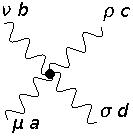
\includegraphics[scale = 0.6]{Vert_A4.jpg} & 
\begin{eqnarray*}
 V_{A^{4}} &=& g^{2} \left[ f^{abe} f^{cde} \left( g_{\mu \rho}g_{\nu \rho} - g_{\mu \sigma}g_{\mu \rho} \right) \right.\\
&& + f^{ace} f^{bde} \left( g_{\mu \nu}g_{\rho \sigma} - g_{\mu \sigma}g_{\rho \nu} \right) \\
&& \left. +f^{ade} f^{cbe} \left( g_{\mu \rho}g_{\sigma \nu} - g_{\mu \nu}g_{\sigma \rho} \right) \right]  \\
\end{eqnarray*}\\
   \hline
   \includegraphics[scale = 0.6]{Vert_CCA.jpg} & 
\begin{equation*}
 V_{ccA} = \frac{-ig}{2}f^{abc}q_{\mu}
\end{equation*}\\
   \hline
\end{tabular}
\end{center}
\caption{Règles de Feynman pour la théorie de Yang Mills}
\end{figure}

%%%%%%%%%%%%%%%%%%%%%%%%%%%%%%%%%%%%%%%%%%%%%%%%%%%%%%%%%%%%%%%%%%%%%%%%%%%%%%%%%%%%%%%%%%%%%%%%%%%%%%%%%%%%%%%%%%%%%%%%%%%%%%%%%%
\section{Symétrie BRST (Becchi, Rouet, Stora, et Tyupkin)}
%%%%%%%%%%%%%%%%%%%%%%%%%%%%%%%%%%%%%%%%%%%%%%%%%%%%%%%%%%%%%%%%%%%%%%%%%%%%%%%%%%%%%%%%%%%%%%%%%%%%%%%%%%%%%%%%%%%%%%%%%%%%%%%%%%


%%%%%%%%%%%%%%%%%%%%%%%%%%%%%%%%%%%%%%%%%%%%%%%%%%%%%%%%%%%%%%%%%%%%%%%%%%%%%%%%%%%%%%%%%%%%%%%%%%%%%%%%%%%%%%%%%%%%%%%%%%%%%%%%%%
\subsection{Définition}
%%%%%%%%%%%%%%%%%%%%%%%%%%%%%%%%%%%%%%%%%%%%%%%%%%%%%%%%%%%%%%%%%%%%%%%%%%%%%%%%%%%%%%%%%%%%%%%%%%%%%%%%%%%%%%%%%%%%%%%%%%%%%%%%%%

\noindent
Lorsque nous avons établi l'expression de la matrice $\mathcal{S}$, le fixage de jauge s'est révélé necessaire. En effet, sans cela 
l'intégrale mise en jeu diverge. Àpres différentes manipulation, nous sommes parvenu à une expression que nous rappeleons ici,

\begin{equation}
 \mathcal{L} = \mathcal{L}_{YM} +\mathcal{L}_{fix.} +\mathcal{L}_{FP}
\end{equation}
où,
\begin{eqnarray}
 && \mathcal{L}_{YM} = \frac{1}{8} tr \left[ F_{\mu \nu}F_{\mu \nu} \right] = \frac{-1}{4} F^{a}_{\mu \nu}F^{a}_{\mu \nu}
\hspace{5mm} \rightarrow \hspace{5mm} \textbf{lagrangien de Yang Mills}\\
 && \mathcal{L}_{fix.} = - \frac{1}{4\alpha} (\partial_{\mu} A_{\mu})^{2} = \frac{1}{2\alpha} (\partial_{\mu} A^{a}_{\mu})^{2}
\hspace{5mm} \rightarrow \hspace{5mm} \textbf{lagrangien fixé de jauge}\\
 && \mathcal{L}_{FP} =  \overline{c}^{a} \left( \Box c^{a} -g f^{abd} \partial_{\mu} \left( A^{b}_{\mu} c^{d} \right) \right)
\hspace{5mm} \rightarrow \hspace{5mm} \textbf{lagrangien des fantômes}
\end{eqnarray}

\noindent
Nous avons précédement montré que $\mathcal{L}_{YM}$ est invariant sous la transformation de jauge de la théorie. Cependant en ayant 
rajouté les termes $\mathcal{L}_{fix.}$ et $\mathcal{L}_{FP} $, la théorie fixée de jauge n'est plus invariante de jauge. Dans ces 
nouveaux termes, on a insérer de nouveaux champs, les famtomes. C. Becchi, A. Rouet, R. Stora, et I. V. Tyupkin ont découvert que 
le lagrangien \textbf{(4.1.1)} possédait encore une symétrie. Cette symétrie est en quelque sorte une symétrie de jauge particulière, 
notée aujourd'hui transformation BRST. \\
Afin de spécifier cette symétrie, il est nécessaire de redéfinir le paramètre de jauge. Nous rappellons que la transformation de jauge 
peut s'écrire comme suit :
\begin{eqnarray}
  A^{\omega}_{\mu} &\simeq& A_{\mu} - [A_{\mu},u] + \partial_{\mu}u + \mathcal{O} (u)
\end{eqnarray}
On va poser $ u = c$. Même si cette découverte a nécéssité un long travail, nous pouvons à posteriori voir la pertinence de cette 
transformation. Faire cette transformation ne va en rien annuler l'invariance de $\mathcal{L}_{YM}$. Mais on peut remarquer que la 
partie $\mathcal{L}_{fix.}$ va insérer des termes proportionnelles aux fantômes, et si nous définissons suffisement astucieusement 
des transformation pour ces fantômes, nous avons des chances d'obtenir que le lagrangien \textbf{(4.1.1)}  soit globalement invariant 
sous ces nouvelles transformations.\\

\noindent
Nous avons donc, 
\begin{eqnarray}
 A^{\omega \hspace{1mm} a}_{\mu}    &\simeq&    A^{a}_{\mu} - f^{abd} A^{a}_{\mu} c^{a} + \partial_{\mu}c^{a}  + \mathcal{O} (c^{a})\\
                                    &\simeq&    A^{a}_{\mu}  + D_{\mu} c^{a} + \mathcal{O} (c^{a})
\end{eqnarray}
\begin{eqnarray}
 \partial_{\mu}  A^{\omega \hspace{1mm} a}_{k}    &\simeq&    \partial_{\mu} A^{a}_{k} - f^{abd}  \partial_{\mu} \left( A^{a}_{k} c^{a} \right) 
+ \Box c^{a} + \mathcal{O} (c^{a})  \\
                                                  &\simeq&     \partial_{\mu} A^{a}_{k}  + \partial_{\mu}D_{\mu} c^{a} + \mathcal{O} (c^{a})
\end{eqnarray}
\begin{eqnarray}
 \left( \partial_{\mu}  A^{\omega \hspace{1mm} a}_{k} \right)^{2} &\simeq&  \left( \partial_{\mu} A^{a}_{k} \right)^{2} 
+ 2 \left(  \partial_{\mu}D_{\mu} c^{a}  \right) \left( \partial_{\mu} A^{a}_{k} \right) + \mathcal{O} (c^{a})  
\end{eqnarray}
On a donc  $\mathcal{L}_{fix.}$ qui se transforme de la façon suivante :
\begin{eqnarray}
 \mathcal{L}_{fix.}  \rightarrow \frac{1}{2 \alpha} \left( \partial_{\mu} A^{a}_{k} \right)^{2} 
+ \frac{1}{\alpha} \left(  \partial_{\mu}D_{\mu} c^{a}  \right) \left( \partial_{\mu} A^{a}_{k} \right) + \mathcal{O} (c^{a})  
\end{eqnarray}
Or on sait que  $\mathcal{L}_{FP}$ peut s'écrire comme :
\begin{eqnarray}
 \mathcal{L}_{FP} &=&  \overline{c}^{a} \left( \Box c^{a} -g f^{abd} \partial_{\mu} \left( A^{b}_{\mu} c^{d} \right) \right) \\
                  &=&  \overline{c}^{a} M  c^{a}
\end{eqnarray}
Si on pose que $\overline{c}$ se transforme comme :
\begin{eqnarray}
 \overline{c}^{a} &\rightarrow& \overline{c}^{a} - \frac{1}{\alpha} \left( \partial_{\mu} A^{a}_{\mu} \right) ,
\end{eqnarray}
on s'aperçoit que l'on va pouvoir compenser le terme $ \delta \mathcal{L}_{fix.} $.
Afin de déterminer  $ \delta c^{a} $, nous allons regarder comment se transforme $D_{\mu}c^{a}$.
\begin{eqnarray}
 D_{\mu}c^{a}  \rightarrow  D_{\mu}c^{a} &+& f^{abd} f^{ben} A^{e}_{\mu} c^{n} c^{d}  +  f^{abd} \left(  \partial_{\mu} c^{b} \right) c^{d}  
\end{eqnarray}
Il n'est pas tout à fait évident de voir que la bonne transformation pour $c^{a}$  est  $c^{a} \rightarrow c^{a} - \frac{1}{2} f^{abd} c^{b} c^{d} $, 
mais nous allons vérifier que cette transformation laisse bien invariant $D_{\mu}c^{a}$.
\begin{eqnarray}
 D_{\mu}c^{a}  \rightarrow  D_{\mu}c^{a} &+& f^{abd} f^{ben} A^{e}_{\mu} c^{n} c^{d}  
+  \frac{1}{2} f^{abd} f^{den} A^{b}_{\mu} c^{e} c^{n}  \nonumber \\
                                         &+& f^{abd} \left(  \partial_{\mu} c^{b} \right) c^{d}  
- \frac{1}{2}  f^{abd}  \left( \partial_{\mu} c^{b} c^{d} \right)  
\end{eqnarray}
Or il existe une propriété sur les constantes de structure de $\cal{G}$, facilement démontrable, qui nous permet d'écrire :
\begin{eqnarray}
 f^{abd} f^{ben} c^{n} c^{d}  = \frac{1}{2} f^{abd} f^{den} c^{e} c^{n}
\end{eqnarray}
De cette remarque nous pouvons en conclure directement ces nouvelles transformations, établies pour $A_{\mu}$, $c$, et $\overline{c}$, laissent 
invariant le lagrangien final \textbf{(4.1.1)}.\\
Résumons ce que l'on va nommer à présent les \textbf{transformations BRST} :
\begin{eqnarray}
 A^{a}_{\mu}    &\rightarrow&    A^{a}_{\mu} - f^{abd} A^{a}_{\mu} c^{a} + \partial_{\mu}c^{a} \\
 \overline{c}^{a} &\rightarrow& \overline{c}^{a} - \frac{1}{\alpha} \left( \partial_{\mu} A^{a}_{\mu} \right) \\
c^{a} &\rightarrow& c^{a} - \frac{1}{2} f^{abd} c^{b} c^{d}
\end{eqnarray}
Il est intéressant de calculer le jacobien de cette transformation, de façon à savoir si la mesure de la matrice $\mathcal{S}$ est invariante ou non.
La matrice jacobienne des transformations BRST est la suivante :
\begin{equation}
J= \left(
 \begin{array}{lcr}
    \delta_{\mu \nu} \delta^{ab}                     & D_{\mu} \delta^{ab}              & 0   \\
    0                                                & \delta^{ab} - f^{adb} c^{d}      & 0   \\
    \delta^{ab} \frac{1}{\alpha}\partial_{\mu}       & 0                                 &\delta^{ab}  
 \end{array} \right).
\end{equation}
Le jacobien vaut donc :
\begin{eqnarray}
 det \left( J \right) = 1.
\end{eqnarray}
On en déduit que la matrice $\mathcal{S}$ est invariante sous les transformations BRST.

%%%%%%%%%%%%%%%%%%%%%%%%%%%%%%%%%%%%%%%%%%%%%%%%%%%%%%%%%%%%%%%%%%%%%%%%%%%%%%%%%%%%%%%%%%%%%%%%%%%%%%%%%%%%%%%%%%%%%%%%%%%%%%%%%%
\subsection{Interprétation géométrique des transformations BRST}
%%%%%%%%%%%%%%%%%%%%%%%%%%%%%%%%%%%%%%%%%%%%%%%%%%%%%%%%%%%%%%%%%%%%%%%%%%%%%%%%%%%%%%%%%%%%%%%%%%%%%%%%%%%%%%%%%%%%%%%%%%%%%%%%%%

\noindent
Il est souvent pratique d'introduire un opérateur différentiel des transformations BRST, couramment noté ''s'', tel que :
\begin{eqnarray}
 \delta A^{a}_{\mu}  &=& s A^{a}_{\mu}  \\
                                   &:=&  D_{\mu} c^{a} \\
 \delta \overline{c}^{a}  &=& s  \overline{c}^{a} \\
                                         &:=& - \frac{1}{\alpha} \left( \partial_{\mu} A^{a}_{\mu} \right) \\
 \delta c^{a} &=& s c^{a} \\
                      &:=& - \frac{1}{2} f^{abd} c^{b} c^{d}
\end{eqnarray}
L'opérateur BRST est nilpotent, c'est à dire $s^2 =0$. \\
Pour le champ de jauge on a :
\begin{eqnarray}
 s^2 A^{a}_{\mu}  &=& s \left( D_{\mu} c^{a} \right) \\
                               &=& \partial_{\mu} s \left( c^{a} \right) + s \left( f^{abd} A^{a}_{\mu} c^{a} \right)  \\
                               &=& \partial_{\mu} s \left( c^{a} \right) +  f^{abd} \left( s A^{a}_{\mu} \right) c^{a} +  f^{abd}  A^{a}_{\mu} 
\left( s c^{a} \right)  \\
                               &=& D_{\mu} (s c^{a} ) +  f^{abd} D_{\mu} (c^{b} ) c^{d} \\
                               &=& D_{\mu} (s c^{a} ) +  \frac{1}{2} D_{\mu}  ( f^{abd} c^{b} c^{d} ) \\
                               &=& D_{\mu} (s c^{a} )  -  D_{\mu}  ( s c^{a} ) \\
 s^2 A^{a}_{\mu} &=& 0.
\end{eqnarray}
Pour le champ des fantômes $c$ on a :
\begin{eqnarray}
 s^2 c^{a} &=& - \frac{1}{2} f^{abd} s ( c^{b} c^{d} ) \\
                  &=& - \frac{1}{2} f^{abd} \left[ (s c^{b} ) c^{d}  - c^{b}  (s c^{d}) \right]\\
                  &=& - \frac{1}{2} f^{abd} \left[  - \frac{1}{2} f^{ben} c^{e}  c^{n}  c^{d} + \frac{1}{2} f^{den} c^{b}  c^{e}  c^{n}  \right]  \\
                  &=& \frac{1}{4} \left[  - f^{abd}  f^{den} c^{b}  c^{e}  c^{n}  +  f^{abd}  f^{ben} c^{e}  c^{n}  c^{d}   \right]\\
                  &=& \frac{1}{2}  f^{abd}  f^{den} c^{e}  c^{n}  c^{b} \\
                  &=& \frac{1}{2}  f^{abd}  f^{end} c^{e}  c^{n}  c^{b} \\
                  &=& \frac{1}{2}  \left(  \delta^{ae}  \delta^{bn} -  \delta^{an}  \delta^{be}  \right)  c^{e}  c^{n}  c^{b}  \\
                  &=& \frac{1}{2}  \left(  c^{a}  c^{b}  c^{b}  -  c^{b}  c^{a}  c^{b}  \right)  \\
                  &=& c^{a}  \left( c^{b}  \right)^{2}  \\
 s^2 c^{a} &=&0.
\end{eqnarray}
On a utilisé l'antisymétrie des constantes de structure de $\cal{G}$, et également le fait que $c$ soit une variable de grassmann. \\
Pour le champ des fantôme $\overline{c}$ on a :
\begin{eqnarray}
 s^2 \overline{c}^{a} &=& - \frac{1}{\alpha} \partial_{\mu} \left( s A_{\mu}c^{a} \right) \\
                                    &=& - \frac{1}{\alpha} \partial_{\mu} D_{\mu} c^{a}
\end{eqnarray}
Or si on applique les équations d'Euler Lagrange en les variables $\overline{c}^{a}$, on obtient l'équation du mouvement suivante :
\begin{eqnarray}
 \partial_{\mu} D_{\mu} c^{a} = 0
\end{eqnarray}
Ce qui implique donc que $s^2 \overline{c}^{a} =0$.\\

\noindent
On a donc bien montré que $s^2 =0 $.\\

\noindent
On va assigner au champ un degré de forme noté $p$, et un degré en fantôme noté $q$. On a en particulier :
\begin{center}
\begin{tabular}{|c|c|c|}
\hline
   Champs & Degré des formes & Degré en fantôme \\
   & p & q \\
\hline
\hline
 $A$ & +1 & 0 \\
\hline
 $c$ & 0 & +1 \\
\hline
 $\overline{c}$ & 0 & -1 \\
\hline
\end{tabular}
\end{center}
Le tenseur $F_{\mu \nu}$ est une forme de degré 2, on peut l'interpréter comme une courbure. Le champ$A_{\mu}$ quand à lui est une forme 
de degré 1, que l'on peut voir comme une connection.\\
On connait les deux dormes différentielles suivantes :
\begin{eqnarray}
 d &:& \Omega^{p,g} \rightarrow \Omega^{p+1,g}\\
 s &:& \Omega^{p,g} \rightarrow \Omega^{p,g+1} ,
\end{eqnarray}
pù $d$ est la difernetielle exterieure, et $s$ la forme differentielle BRST.\\
Avec ces formes différentielles, on écrit $F$ de la façon suivante :
\begin{eqnarray}
 F = dA + \frac{1}{2} [A,A] ,
\end{eqnarray}
où $F$ vérifie l'équation de Bianchi :
\begin{eqnarray}
 DF = dF + [A,F] = 0 ,
\end{eqnarray}
qui est en fait l'équation du mouvement de la théorie non fixée de jauge.
On construit une nouvelle connection $\tilde{A}$ et une nouvelle courbure $\tilde{F}$ tel que :

\begin{eqnarray}
 \tilde{A}  &:=& A^{1,0} + c^{0,1}\\
 \tilde{F}  &:=& \tilde{d} \tilde{A}^{1,1} + \frac{1}{2} \left[ \tilde{A}^{1,1} , \tilde{A}^{1,1} \right]\\
            &=& dA^{1,0} + dc^{0,1} + sA^{1,0} + sc^{0,1} \nonumber \\ &&  
+ \frac{1}{2} \left( [A^{1,0},A^{1,0}] + [c^{0,1},c^{0,1}] + [c^{0,1},A^{1,0}]  + [A^{1,0},c^{0,1}] \right) \\ 
            &=& dA^{1,0} + dc^{0,1} + sA^{1,0} + sc^{0,1} \nonumber \\ &&  
+ \frac{1}{2} \left( [A^{1,0},A^{1,0}] + [c^{0,1},c^{0,1}]  \right) +  [A^{1,0},c^{0,1}] \\ 
 \tilde{F}  &=& \left( dA^{1,0} + \frac{1}{2}[A^{1,0},A^{1,0}] \right)^{2,0}  
+ \left( sc^{0,1} + \frac{1}{2} [c^{0,1},c^{0,1}] \right)^{0,2}   \nonumber \\ 
&& + \left( dc^{0,1} + sA^{1,0} + [A^{1,0},c^{0,1}] \right)^{1,1}
\end{eqnarray}
Considérer $\tilde{F}$ illustre en quelque sorte le fixage de jauge. On a utilisé le fait que le crochet $[,]$ est gradué, et donc lorsque 
nous avions $[c^{0,1},A^{1,0}]$, le degré total étant égale à deux, ce crochet est danc ce cas un anticommutateur. 
On a  $[c^{0,1},A^{1,0}] =  [c^{0,1},A^{1,0}]$. En imposant   $\tilde{F} := F$ on obtient les deux relations suivante :
\begin{eqnarray}
  && sc = - \frac{1}{2} \left[ c , c \right] \\
  && sA = - \left( dc + [A,c] \right) = Dc ,
\end{eqnarray}
qui sont deux des transformations BRST.

%%%%%%%%%%%%%%%%%%%%%%%%%%%%%%%%%%%%%%%%%%%%%%%%%%%%%%%%%%%%%%%%%%%%%%%%%%%%%%%%%%%%%%%%%%%%%%%%%%%%%%%%%%%%%%%%%%%%%%%%%%%%%%%%%%
\section{Identités de Slavnov}
%%%%%%%%%%%%%%%%%%%%%%%%%%%%%%%%%%%%%%%%%%%%%%%%%%%%%%%%%%%%%%%%%%%%%%%%%%%%%%%%%%%%%%%%%%%%%%%%%%%%%%%%%%%%%%%%%%%%%%%%%%%%%%%%%%

\noindent
Les identités de Slavnov sont les identités de Ward de l'electrodynamque, généralisée au champ de Yang Mills. 
Il important de noter que ces identités sont des relations entre les fonctions de corrélations qui découlent des symétries de la théorie. 
Ces identités sont toujours valable apres renormalisation. Elles sont une version quantique du théorme de Noether.\\

\noindent
Pour la théorie de Yang Mills fixée de jauge, on a l'action :
\begin{eqnarray}
 \mathcal{I} =  \int \left[ 
\frac{-1}{4} F^{a}_{\mu\nu}(x)F^{a}_{\mu \nu}(x) + \overline{c}^{a}(x)M^{ab}c^{b}(x) + \frac{1}{\alpha} (\partial_{\mu}A_{\mu})^2  
\right] dx 
\end{eqnarray}

\noindent
Comme nous l'avons vu dans la partie \textbf{(4)}, cette action est invariante sous les transformations BRST \textbf{(4.19-21)}, 
que l'on réécrit comme :
\begin{eqnarray}
 A_{\mu}^{a} \rightarrow  A_{\mu}^{a} + \delta  A_{\mu}^{a}   \hspace{5mm}  &\text{avec}&   \hspace{5mm}  \delta  A_{\mu}^{a} := s  A_{\mu}^{a} \\
 c^{a}  \rightarrow  c^{a}  + \delta  c^{a}   \hspace{5mm}  &\text{avec}&   \hspace{5mm}    \delta  c^{a} := s  c^{a}  \\
 \overline{c}^{a}  \rightarrow  \overline{c}^{a}  + \delta  \overline{c}^{a}   \hspace{5mm}  &\text{avec}&   \hspace{5mm} 
\delta  \overline{c}^{a} := s  \overline{c}^{a}  .
\end{eqnarray}
Nous allons écrire la fonctionnelle génératrice des fonctions de Green $Z$, avec $ J_{\mu}^{a}$ source des champs de jauge $A_{\mu}^{a}$, 
$\overline{\xi}^{a}$ source des champs de jauge de $c^{a}$,  $\xi^{a}$ source des champs de jauge de $\overline{c}^{a}$, $k^{\mu}_{a}$ source 
de $sA^{\mu}_{a}$, et $l^{a}$ source de $sc^{a}$.
\begin{eqnarray}
 \mathcal{Z} &=& \int exp\left( i \int \left[
\frac{-1}{4g} F^{a}_{\mu\nu}(x)F^{a}_{\mu \nu}(x) + \overline{c}^{a}(x)M^{ab}c^{b}(x) 
+ \frac{1}{\alpha}(\partial_{\mu}A_{\mu}^{a})^2 \right. \right. \nonumber \\
     &+& \left. \left. J_{\mu}^{a}A_{\mu}^{a} + \overline{\xi}^{a}c^{a} + \overline{c}^{a}\xi^{a} + k^{\mu}_{a}sA^{\mu}_{a} 
+ l^{a}sc^{a} \right] dx \right) dA_{\mu} dc d\overline{c} 
\end{eqnarray}
À présent nous allons regarder comment se comporte cette fonctionnelle génératrice des focntions de Green sous les transformations BRST. Sachant que $\mathcal{I}$ est invarainte, et que $s^2=0$, les seules termes additionnels sont issue des termes de source $A_{\mu}^{a}$, $c^{a}$, et $\overline{c}^{a}$.
\begin{eqnarray}
 \mathcal{Z} &\rightarrow&  exp \left( i \int \left[ J_{\mu}^{a} s A_{\mu}^{a} + \overline{\xi}^{a} s c^{a} + s \overline{c}^{a} \xi^{a} \right] dx \right)  \mathcal{Z}
\end{eqnarray}
En imposant que $\mathcal{Z}$ soit invariante sous les tranformations BRST, il vient :
\begin{eqnarray}
\int \left[ J_{\mu}^{a} s A_{\mu}^{a} + \overline{\xi}^{a} s c^{a} + s \overline{c}^{a} \xi^{a} \right] dx  & \mathcal{Z}&  = 0.
\end{eqnarray}
En utilisantla notion de dérivée fonctionnelle, on peut réécrire cette relation comme suit :
\begin{eqnarray}
\int \left[ J_{\mu}^{a} \frac{\delta}{i \delta k^{a}_{\mu} } - \overline{\xi}^{a} \frac{\delta}{i \delta l^{a} }  
- \frac{1}{\alpha} \left( \partial_{\mu} A_{\mu}^{a} \right) \xi^{a} \right] dx  & \mathcal{Z}&  = 0 \\
\int \left[ J_{\mu}^{a} \frac{\delta}{i \delta k^{a}_{\mu} } - \overline{\xi}^{a} \frac{\delta}{i \delta l^{a} }  
- \frac{1}{\alpha} \xi^{a}  \partial_{\mu} \frac{\delta}{i \delta J_{\mu}^{a} }  \right] dx  & \mathcal{Z}&  = 0
\end{eqnarray}
Cette relation est ce que l'on appelle l'identité de Slavnov obtenue à partir de la symétrie BRST. 
On pose,
\begin{eqnarray}
 && W = i \int \mathcal{L} dx  \nonumber  \\
 && \text{c'est à dire} \hspace{2mm} W = ln ( \mathcal{Z} ) 
\end{eqnarray}
On a alors :
\begin{eqnarray}
 \int dx \left[ J^{a}_{\mu} \frac{\delta}{i \delta k^{a}_{\mu}} - \overline{\xi^{a}} \frac{\delta}{i \delta l^{a}} - \frac{1}{\alpha} 
\xi^{a} \partial_{\mu} \frac{\delta}{i \delta J^{a}_{\mu}}\right] &W& =0
\end{eqnarray}
On écrit $\Gamma$, fonction de corréaltion, à l'aide de $W$, de la façon suivante :
\begin{eqnarray}
 \Gamma &=& -iW - \int dx \left(J_{\mu}^{a}A_{\mu}^{a} + \overline{\xi}^{a}sc^{a} + s\overline{c}^{a}\xi^{a} \right) ,
\end{eqnarray}
ce qui nous permet encore d'écrire :
\begin{eqnarray}
 && \int dx \left[ -\frac{\delta \Gamma}{\delta A^{a}_{\mu}} \frac{\delta G }{i \delta k^{a}_{\mu}} 
- \frac{\delta \Gamma}{c^{a}}\frac{\delta G}{i \delta l^{a}} 
+ \frac{1}{\alpha} \left( \partial_{\mu} A^{a}_{\mu} \right) \frac{\delta \Gamma}{\delta \overline{c^{a}}}\right] = 0 ,  \\
 && \int dx \left[ -\frac{\delta \Gamma}{\delta A^{a}_{\mu}} \frac{\delta \Gamma }{i \delta k^{a}_{\mu}} 
- \frac{\delta \Gamma}{c^{a}}\frac{\delta \Gamma}{i \delta l^{a}} 
+ \frac{1}{\alpha} \left( \partial_{\mu} A^{a}_{\mu} \right) \frac{\delta \Gamma}{\delta \overline{c^{a}}}\right] = 0 .
\end{eqnarray}
Cette derniere équation est l'équation de Zin-Justin. Afin de prouver la renormalisabilité de la théorie de Yang Mills à tous les ordres, 
on s'apercevra de l'utilité d'avoir écrit l'identité de Slavnov en fonction de $\Gamma$.
En posant :
\begin{eqnarray}
 \Gamma = \Gamma + \frac{1}{2 \alpha} \int dx \left( \partial_{\mu} A^{a}_ {\mu} \right)^{2},
\end{eqnarray}
on peut réécrire l'equation de Zinn-Justin de façon plus commode pour la suite,
\begin{eqnarray}
 \int dx \left[ \frac{\delta \Gamma}{\delta A^{a}_{\mu}} \frac{\delta G }{i \delta k^{a}_{\mu}} 
+ \frac{\delta \Gamma}{c^{a}}\frac{\delta G}{i \delta l^{a}} \right] = 0.
\end{eqnarray}

%%%%%%%%%%%%%%%%%%%%%%%%%%%%%%%%%%%%%%%%%%%%%%%%%%%%%%%%%%%%%%%%%%%%%%%%%%%%%%%%%%%%%%%%%%%%%%%%%%%%%%%%%%%%%%%%%%%%%%%%%%%%%%%%%%
\section{Renormalisation}
%%%%%%%%%%%%%%%%%%%%%%%%%%%%%%%%%%%%%%%%%%%%%%%%%%%%%%%%%%%%%%%%%%%%%%%%%%%%%%%%%%%%%%%%%%%%%%%%%%%%%%%%%%%%%%%%%%%%%%%%%%%%%%%%%%


%%%%%%%%%%%%%%%%%%%%%%%%%%%%%%%%%%%%%%%%%%%%%%%%%%%%%%%%%%%%%%%%%%%%%%%%%%%%%%%%%%%%%%%%%%%%%%%%%%%%%%%%%%%%%%%%%%%%%%%%%%%%%%%%%%
\subsection{Calcul d'un diagramme de Feynman}
%%%%%%%%%%%%%%%%%%%%%%%%%%%%%%%%%%%%%%%%%%%%%%%%%%%%%%%%%%%%%%%%%%%%%%%%%%%%%%%%%%%%%%%%%%%%%%%%%%%%%%%%%%%%%%%%%%%%%%%%%%%%%%%%%%

\noindent
Maintenant que l'on a déterminé les règles de Feynman, on va pouvoir calculer l'amplitude d'un diagramme. On considére le diagramme suivant :
\begin{figure}[H]
 \begin{center}
  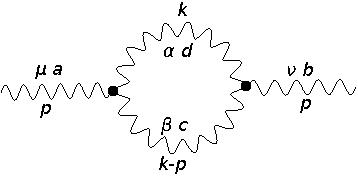
\includegraphics[scale=0.4]{1_loop_2_vert_3A.jpg}
 \end{center}
\end{figure}

\noindent
En appliquant les règles de Feynman, on obtient :
\begin{eqnarray}
 \Pi^{ab}_{\mu\nu}(p) &=& - i g^{2}  \int \frac{d^{4}k}{\left(2\pi\right)^4} f^{ad_{1}c_{1}} 
\left[(-p-k)_{\beta_{1}}g_{\mu\alpha_{1}}  +  (k+k-p)_{\mu}g_{\alpha_{1}\beta_{1}}  +  (-k+p+p)_{\alpha_{1}}g_{\beta_{1}\mu}  \right]. \nonumber \\
&& f^{d_{2}bc_{2}} \left[(-k-p)_{\beta_{2}}g_{\alpha_{2}\nu}  +  (p-k+p)_{\alpha_{2}}g_{\nu\beta_{2}}  
+  (k-p+k)_{\nu}g_{\beta_{1}\alpha{1}}  \right].\nonumber  \\
&& \frac{-i\delta^{d_{1}d_{2}}g_{\alpha_{1}\alpha_{2}}}{k^2+i0} . \frac{-i\delta^{c_{1}c_{2}}g_{\beta_{1}\beta_{2}}}{(k-p)^2+i0}  .
\end{eqnarray}
Ce que l'on peut encore écrire comme :
\begin{eqnarray}
 \Pi^{ab}_{\mu\nu}(p) &=&  - i g^{2}  \delta^{ab} \int \frac{d^{4}k}{\left(2\pi\right)^4} 
[g_{\mu\nu}\left((p+k)^{2} +(k-2p)^2\right) + p_{\mu}p_{\nu}\left(n-6\right)+k_{\mu}k_{\nu}\left(4n-6\right)  \nonumber  \\
&&  +(3-2n)(p_{\nu}k_{\mu}+p_{\mu}k_{\nu})]\frac{1}{k^2+i0}\frac{1}{(k-p)^2+i0}
\end{eqnarray}
Lorsque $k \to 0$, on s'aperçoit que cette intégrale diverge. Ce qui est sérieux problème pour notre théorie. On ne peut attribuer un sens 
physique à cette intégrale, pour l'instant du moins.\\

\noindent
Pour remédier à ce problème nous allons devoir renormaliser notre thèorie. On va pour cela proceder en plusieurs étapes. On va tout d'abord 
identifier les diagrammes divergents, en utilisant la méthode du comptage en puissance. Ensuite nous régulariserons les intégrales divergentes, 
en ajoutant un paramètres qui va ''absorber'' les divergences. Et pour finir nous pourrons construire des termes de compensations pour ces 
divergences dans le lagrangien de départ, c'est ce qu'on nomme habituelement les contres termes.

%%%%%%%%%%%%%%%%%%%%%%%%%%%%%%%%%%%%%%%%%%%%%%%%%%%%%%%%%%%%%%%%%%%%%%%%%%%%%%%%%%%%%%%%%%%%%%%%%%%%%%%%%%%%%%%%%%%%%%%%%%%%%%%%%%
\subsection{Comptage en puissance}
%%%%%%%%%%%%%%%%%%%%%%%%%%%%%%%%%%%%%%%%%%%%%%%%%%%%%%%%%%%%%%%%%%%%%%%%%%%%%%%%%%%%%%%%%%%%%%%%%%%%%%%%%%%%%%%%%%%%%%%%%%%%%%%%%%


%%%%%%%%%%%%%%%%%%%%%%%%%%%%%%%%%%%%%%%%%%%%%%%%%%%%%%%%%%%%%%%%%%%%%%%%%%%%%%%%%%%%%%%%%%%%%%%%%%%%%%%%%%%%%%%%%%%%%%%%%%%%%%%%%%
\subsubsection{Définition}
%%%%%%%%%%%%%%%%%%%%%%%%%%%%%%%%%%%%%%%%%%%%%%%%%%%%%%%%%%%%%%%%%%%%%%%%%%%%%%%%%%%%%%%%%%%%%%%%%%%%%%%%%%%%%%%%%%%%%%%%%%%%%%%%%%

\noindent
On établie tout d'abord quelques notations :
\begin{itemize}
\renewcommand{\labelitemi}{$\cdot$}
 \item $q$ : nombre de vertex considéré
 \item $n$ : nombre total de vertex
 \item $l$ : nombre de ligne interne considéré
 \item $L$ : nombre total de vertex
 \item $m$ : nombre de dérivée à chaque vertex
 \item $d$ : dimension
\end{itemize}
L'amplitude s'écrit typiquement comme :
\begin{eqnarray}
 J(k)= \int \prod_{ {1\le q\le n\atop} } \delta \left( \sum p - k_{q} \right) \prod_{1\le l\le L\atop} D_{l}(p_{l}) d_{p_{l}}
\end{eqnarray}
avec $D_{l}(p_{l})$ la fonction de Green qui à la forme suivante :
\begin{eqnarray}
 D_{l}(p_{l}) = \frac{Z(p_{l})}{ m_{l}^{2}-p_{l}^{2}  }
\end{eqnarray}
où $Z$ est un polynôme en $p_{l}$ de degré $r_{l}$.\\
L'amplitude doit rester fini pour n'importe quel valeur de $k$ et $p$. De ce fait on modifie les paramètres par un facteur d'echelle $a$ 
afin de voir comment va se comporter l'amplitude sous cette modification.
\begin{eqnarray}
 p_i , k_i \rightarrow a p_i , a k_i
\end{eqnarray}
Si J converge , J sera multiplié par $a^{\omega}$, où $\omega$ est appelé l'index.
\begin{itemize}
\renewcommand{\labelitemi}{$\cdot$}
 \item $\omega > 0$, le comptage en puissance prévoit une divergence.
 \item $\omega = 0$, le comptage en puissance prévoit une divergence logaritmique.
 \item $\omega < 0$, c'est sûr ça converge !
\end{itemize}
Ça caratérise la situation la plus défavorable, il peut y avoir des cas où le comptage en puissance prédit une divergence mais 
où en réalité l'amplitude converge !\\
\begin{eqnarray}
 \omega &=& \sum_{{1\le l\le L\atop}} (r_{l}-2) + d(L-(n-1)) + n.m\\
 &=& \sum_{{1\le l\le L\atop}} (r_{l}-2+d) - d(n-1) + n.m
\end{eqnarray}

%%%%%%%%%%%%%%%%%%%%%%%%%%%%%%%%%%%%%%%%%%%%%%%%%%%%%%%%%%%%%%%%%%%%%%%%%%%%%%%%%%%%%%%%%%%%%%%%%%%%%%%%%%%%%%%%%%%%%%%%%%%%%%%%%%
\subsubsection{Identification des diagrammes divergents}
%%%%%%%%%%%%%%%%%%%%%%%%%%%%%%%%%%%%%%%%%%%%%%%%%%%%%%%%%%%%%%%%%%%%%%%%%%%%%%%%%%%%%%%%%%%%%%%%%%%%%%%%%%%%%%%%%%%%%%%%%%%%%%%%%%

\noindent
On est à présent  dans le cas de Yang-Mills, on considère alors :
\begin{itemize}
\renewcommand{\labelitemi}{$\cdot$}
 \item $L^{A}_{in}$ : nombre de ligne interne de $A$.
 \item $L^{c}_{in}$ : nombre de ligne interne de $c$.
 \item $L^{A}_{ex}$ : nombre de ligne externe de $A$.
 \item $L^{c}_{ex}$ : nombre de ligne externe de $c$.
 \item $n_{4}$ : nombre total de vertex $AAAA$.
 \item $m_{4}$ : nombre de dérivée à chaque vertex $AAAA$, ici $m_{4}=0$.
 \item $n_{3}$ : nombre total de vertex $AAA$.
 \item $m_{3}$ : nombre de dérivée à chaque vertex $AAA$, ici $m_{3}=1$.
 \item $n_{c}$ : nombre total de vertex $c$.
 \item $m_{c}$ : nombre de dérivée à chaque vertex $c$, ici $m_{c}=1$.
 \item $r_{l}=0$ : degré de $Z$.
\end{itemize}

\begin{eqnarray}
 \omega &=& 2L^{A}_{in} + 2L^{c}_{in} - d(n_{4}+n_{3}+n_{c}-1)+ n_{4}m_{4} + n_{3}m_{3} + n_{c}m_{c}\\
        &=& 2L^{A}_{in} + 2L^{c}_{in} + d - n_{4} d -n_{3} (d-1)- n_{c} (d-1)
\end{eqnarray}
de plus on a :
\begin{eqnarray}
 2L^{A}_{in} + L^{A}_{ex} &=& 4n_{4}+3n_{3}+n_{c}\\
 2L^{c}_{in} + L^{c}_{ex} &=& 2n_{c}
\end{eqnarray}
et donc :
\begin{eqnarray}
 \omega &=& d -L^{A}_{ex}-L^{c}_{ex} - n_{4} (d-4) - n_{3} (d-4) - n_{c} (d-4)
\end{eqnarray}
On remarque que dans le cas particulier $d=4$, $\omega$ depend uniquement du nombre de ligne externe. On a donc montré dans ce cas 
la relation suivante :
\begin{eqnarray}
 \omega &=& 4-L^{A}_{ex}-L^{c}_{ex}
\end{eqnarray}
Les seules diagrammes divergents dans la théorie de Yang Mills sont donc les suivants :
\begin{figure}[H]
\begin{center}
\begin{tabular}{|c|c|}
   \hline
   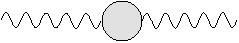
\includegraphics[scale = 0.6]{graph_1_div.jpg} & $\omega$ = 2\\
   \hline
   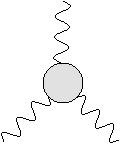
\includegraphics[scale = 0.6]{graph_2_div.jpg} & $\omega$ = 1\\
   \hline
   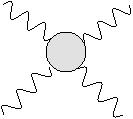
\includegraphics[scale = 0.6]{graph_3_div.jpg} & $\omega$ = 0\\
   \hline
   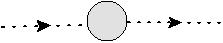
\includegraphics[scale = 0.6]{graph_4_div.jpg} & $\omega$ = 2\\
   \hline
   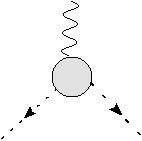
\includegraphics[scale = 0.6]{graph_5_div.jpg} & $\omega$ = 1\\
   \hline
\end{tabular}
\end{center}
\caption{Diagrammes divergents pour la théorie de Yang Mills pure}
\end{figure}

\noindent
On a réduit sensiblement le nombre de possibilité de divergence. 

%%%%%%%%%%%%%%%%%%%%%%%%%%%%%%%%%%%%%%%%%%%%%%%%%%%%%%%%%%%%%%%%%%%%%%%%%%%%%%%%%%%%%%%%%%%%%%%%%%%%%%%%%%%%%%%%%%%%%%%%%%%%%%%%%%
\subsection{Régularisation dimensionnelle}
%%%%%%%%%%%%%%%%%%%%%%%%%%%%%%%%%%%%%%%%%%%%%%%%%%%%%%%%%%%%%%%%%%%%%%%%%%%%%%%%%%%%%%%%%%%%%%%%%%%%%%%%%%%%%%%%%%%%%%%%%%%%%%%%%%


%%%%%%%%%%%%%%%%%%%%%%%%%%%%%%%%%%%%%%%%%%%%%%%%%%%%%%%%%%%%%%%%%%%%%%%%%%%%%%%%%%%%%%%%%%%%%%%%%%%%%%%%%%%%%%%%%%%%%%%%%%%%%%%%%%
\subsubsection{Définition}
%%%%%%%%%%%%%%%%%%%%%%%%%%%%%%%%%%%%%%%%%%%%%%%%%%%%%%%%%%%%%%%%%%%%%%%%%%%%%%%%%%%%%%%%%%%%%%%%%%%%%%%%%%%%%%%%%%%%%%%%%%%%%%%%%%

\noindent
Plusieurs méthodes de régularisation existent, celle que nous privilégions ici est la régularisation dimenssionnelle. Dans la majorité 
des cas, la technique de régularisation consiste à inserer un paramètre de regularisation, de façon à ce que les intégrales à calculer 
soit des des fonctions analytiques de ce paramètre dans un certain domaine. L'idée est un peu la même pour la régularisation dimenssionnelle, 
sauf que dans ce cas le paramètre de régularisation est la dimension elle même. Il s'avère qu'en prolongeant l'intégration dans le plan 
complexe, l'intégrale correspondante devient convergente.\\
Dans le paraggraphe \textbf{6.1} on a pu remarqué que l'on a des intégrales divergentes de la forme :
\begin{eqnarray}
 J(d,k) = \int d^{4}p f(p,k).
\end{eqnarray}
L'idée de la régularisation dimenssionnelle est d'utiliser la dimension du domaine d'intégration comme paramètre de régularisation, 
afin de rendre $J$ convergente. En particulier on ne va plus intégrer sur l'espace réel, mais on va prolonger analytiquement le domaine 
d'intégration sur le plan complexe. Pour rendre ces intégrales convergentes on va proceder de la mainiere suivante :
\begin{itemize}
 \renewcommand{\labelitemi}{$\cdot$}
 \item Il nous faudra trouver le domaine de convergence pour $Re(d)<4$.
 \item On va construire une fonction égale à notre intégrale de départ ($J$) pour $d=4$, mais définie dans un domaine plus grand qui 
inclu le domaine $d=4$.
 \item Et pour finir on prendra $d \rightarrow 4$ pour isoler la singularité. Et ainsi on poura constrire le contre terme à ajouter dans le 
lagangien pour rendre la théorie finie.
\end{itemize}

\noindent
Pour définir la régularisation dimenssionnelle nous nous donnons ces trois conditions :
\begin{enumerate}
\item translation
          \begin{eqnarray}
           \int d^{d}p F(p+q) = \int d^{d}p F(p)
          \end{eqnarray}
\item expansion
          \begin{eqnarray}
           \int d^{d}p F(a.p) = |a^{-d} | \int d^{d}p F(p)
          \end{eqnarray}
\item factorisation
          \begin{eqnarray}
           \int d^{d_1}p d^{d_2}q f(p) g(q) = \int d^{d_1}p f(p)  \int d^{d_2}p g(q)
          \end{eqnarray}
\end{enumerate}

\noindent
Nous remarquons en particulier que la propriété  \textbf{2} implique :
\begin{eqnarray}
 \int d^{d}p = 0 \hspace{2mm} ;  \hspace{2mm} \int \frac{d^{d}p}{p^2} = 0 \hspace{2mm} ;  \hspace{2mm} ...
\end{eqnarray}

%%%%%%%%%%%%%%%%%%%%%%%%%%%%%%%%%%%%%%%%%%%%%%%%%%%%%%%%%%%%%%%%%%%%%%%%%%%%%%%%%%%%%%%%%%%%%%%%%%%%%%%%%%%%%%%%%%%%%%%%%%%%%%%%%%
\subsubsection{Régularisation à 1 boucle}
%%%%%%%%%%%%%%%%%%%%%%%%%%%%%%%%%%%%%%%%%%%%%%%%%%%%%%%%%%%%%%%%%%%%%%%%%%%%%%%%%%%%%%%%%%%%%%%%%%%%%%%%%%%%%%%%%%%%%%%%%%%%%%%%%%


\noindent
On va travailler avec des intégrales de la formes : 
\begin{eqnarray}
 J(n) = \int d^{n}k f(k^2)
\end{eqnarray}
Afin de simplifier le calcul on passe en coordonnée polaires : 
\begin{eqnarray}
 \left( k_{1} , ... , k_{n} \right) \rightarrow \left( k, \Phi, \theta_{1}, ... , \theta_{n-2} \right)
\end{eqnarray}
avec :
\begin{eqnarray}
 && 0 \leq k \leq + \infty \\
 && 0 \leq \Phi \leq 2 \pi \\
 && 0 \leq \theta_{i} \leq \pi \\
\end{eqnarray}
On a alors :
\begin{eqnarray}
 J(n) &=& 2 \pi  \prod_{l=1}^{n-2} \int_{0}^{\pi} sin^{l}(\theta_{l}) d\theta_{l}  \int_{0}^{+\infty} dk k^{n-1} f(k^2)
\end{eqnarray}
or on sait que :
\begin{eqnarray}
 \int_{0}^{\pi} sin^{l}(\theta_{l}) d\theta_{l}   &=& \sqrt{\pi} \frac{\Gamma(\frac{l+1}{2})}{\Gamma(1+\frac{l}{2})}
\end{eqnarray}
donc,
\begin{eqnarray}
 J(n) &=& \frac{2 \pi ^{\frac{n}{2}}}{\Gamma(\frac{n}{2})} \int_{0}^{+\infty} dk k^{n-1} f(k^2)
\end{eqnarray}
Dans la suite on sera amené à utilisé la formule suivante :
\begin{eqnarray}
 B(x,y) &=& \int_{0}^{1} dz z^{x-1} (1-z)^{y-1} \\
            &=& \int_{0}^{+\infty}  dt t^{x-1} (1+t)^{-x-y} \\
            &=& \frac{\Gamma(x) \Gamma(y)}{\Gamma(x+y)}
\end{eqnarray}

\noindent
\underline{\textbf{Diagramme à une Boucle en les champs de jage $A_{\mu}$}}

\begin{figure}[H]
 \begin{center}
  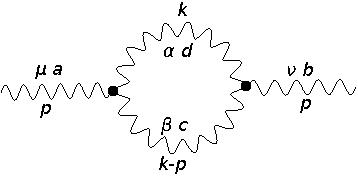
\includegraphics[scale=0.4]{1_loop_2_vert_3A.jpg}
 \end{center}
\end{figure}

\noindent
Grâce aux régles de feynman précédément établies, on a réussi à écrire la fonction deux points correspondantes. On se place maintenant 
dans le cas n-dimenssionnel. Pour conserver la bonne dimension de la fonction de correlation on a introduit la constante de 
couplage $\tilde{g}^{2} = g^{2} \mu^{4-n}$.

\begin{eqnarray}
 \Pi^{ab}_{\mu\nu}(p) &=& -\tilde{g}^{2}  \int \frac{d^{n}k}{\left(2\pi\right)^n} f^{ad_{1}c_{1}} 
\left[(-p-k)_{\beta_{1}}g_{\mu\alpha_{1}}  +  (k+k-p)_{\mu}g_{\alpha_{1}\beta_{1}}  +  (-k+p+p)_{\alpha_{1}}g_{\beta_{1}\mu}  \right]. \nonumber \\
&& f^{d_{2}bc_{2}} \left[(-k-p)_{\beta_{2}}g_{\alpha_{2}\nu}  +  (p-k+p)_{\alpha_{2}}g_{\nu\beta_{2}}  
+  (k-p+k)_{\nu}g_{\beta_{1}\alpha{1}}  \right].\nonumber  \\
&& \frac{-i\delta^{d_{1}d_{2}}g_{\alpha_{1}\alpha_{2}}}{k^2+i0} . \frac{-i\delta^{c_{1}c_{2}}g_{\beta_{1}\beta_{2}}}{(k-p)^2+i0} 
\end{eqnarray}
Ce que l'on peut encore écrire comme :
\begin{eqnarray}
 \Pi^{ab}_{\mu\nu}(p)      &=&  -\tilde{g}^{2} \int \frac{d^{n}k}{\left(2\pi\right)^n} f^{adc} f^{bdc}
\left[  (p+k)_{\beta}g_{\mu\alpha}  +  (p-2k)_{\mu}g_{\alpha\beta}  +  (k-2p)_{\alpha}g_{\beta\mu}  \right].   \nonumber  \\
&& \left[  (k+p)_{\beta} g_{\alpha\nu}  +  (k-2p)_{\alpha}g_{\nu\beta}  +  (p-2k)_{\nu}g_{\beta\alpha}  \right]  
\frac{1}{k^2+i0} . \frac{1}{(k-p)^2+i0}\\
                      &=&  -\tilde{g}^{2}  \delta^{ab} \int \frac{d^{n}k}{\left(2\pi\right)^n} 
[  (p+k)^{2}g_{\mu\nu}  +  (p+k)_{\nu}(k-2p)_{\mu}  +  (p+k)_{\mu}(p-2k)_{\nu}  \nonumber  \\
&&  +  (p-2k)_{\mu}(k+p)_{\nu}  +  (p-2k)_{\mu}(k-2p)_{\nu}  +  (p-2k)_{\mu}(p-2k)_{\nu}g_{\alpha\beta}g_{\beta\alpha}  \nonumber  \\
&&  +  (k-2p)_{\nu}(k+p)_{\mu}  +  (k-2p)^2g_{\nu\mu}  +  (k-2p)_{\mu}(p-2k)_{\nu}  ] \nonumber  \\
&&  \frac{1}{k^2+i0} . \frac{1}{(k-p)^2+i0}
\end{eqnarray}
On a alors finalement :
\begin{eqnarray}
 \Pi^{ab}_{\mu\nu}(p) &=&  -\tilde{g}^{2}  \delta^{ab} \int \frac{d^{n}k}{\left(2\pi\right)^n} 
[g_{\mu\nu}\left((p+k)^{2} +(k-2p)^2\right) + p_{\mu}p_{\nu}\left(n-6\right)+k_{\mu}k_{\nu}\left(4n-6\right)  \nonumber  \\
&&  +(3-2n)(p_{\nu}k_{\mu}+p_{\mu}k_{\nu})]\frac{1}{k^2+i0}\frac{1}{(k-p)^2+i0}
\end{eqnarray}
On remarque que l'intégrale converge pour $n<0$, et diverge pour $n>0$.\\

\noindent
Pour écrire le dénominateur sous un seul facteur, on utilise une des formules de feynman,
\begin{eqnarray}
 \frac{1}{k^2+(p-k)^2} = \int_0^{1} dz \frac{1}{\left[k^2(1-z)+(p-k)^2z\right]^2}
\end{eqnarray} 
Ce qui nous permet d'écrire :
\begin{eqnarray}
 \Pi^{ab}_{\mu\nu}(p) &=&  -\tilde{g}^{2}  \delta^{ab} \int_0^{1} dz \int \frac{d^{n}k}{\left(2\pi\right)^n} 
\left( g_{\mu\nu}\left((p+k)^{2} +(k-2p)^2\right) + p_{\mu}p_{\nu}\left(n-6\right)+k_{\mu}k_{\nu}\left(4n-6\right)\right.\nonumber    \\
&+& \left. (3-2n)(p_{\nu}k_{\mu}+p_{\mu}k_{\nu}) \right) \frac{1}{\left[k^2(1-z)+(p-k)^2z\right]^2}
\end{eqnarray}
Afin d'élinminer les termes linéaires en $k$, on effectue le changement de varaiable suivant :
\begin{eqnarray}
 k \rightarrow k+pz
\end{eqnarray}
d'où,
\begin{eqnarray}
 \Pi^{ab}_{\mu\nu}(p) &=&  -\tilde{g}^{2}  \delta^{ab} \int_0^{1} dz \int \frac{d^{n}k}{\left(2\pi\right)^n} 
\left(g_{\mu\nu} (5-2z+2z^2)p^2 + 2g_{\mu\nu}k^2 + (4n-6)k_{\mu}k_{\nu}\right. \nonumber  \\
&& \left. -(4n-6)z(1-z)p_{\mu}p_{\nu} +(n-6)p_{\mu}p_{\nu}  \right)
\frac{1}{\left[k^2 + p^2 z (1-z) \right]^2} 
\end{eqnarray}
Comme nous l'avons fait pour le cas générique de l'intégrale $J$ nous allons passer en coordonnée polaire, ce qui nous donne :
\begin{eqnarray}
 \Pi^{ab}_{\mu\nu}(p) &=&  -\tilde{g}^{2}  \delta^{ab}  \frac{2 \pi^{\frac{n}{2}}}{\Gamma(\frac{n}{2})}  \int_0^{1} dz 
\int \frac{dk}{\left(2\pi\right)^n} k^{n-1}
\left(g_{\mu\nu} (5-2z+2z^2)p^2 + 2g_{\mu\nu}k^2 + (4n-6)k_{\mu}k_{\nu}\right. \nonumber  \\
&& \left. -(4n-6)z(1-z)p_{\mu}p_{\nu} +(n-6)p_{\mu}p_{\nu}  \right)
\frac{1}{\left[k^2 + p^2 z (1-z) \right]^2} 
\end{eqnarray}
En utilisant la formule \textbf{(6.3.15-17)} pour les intégration sur k et z, on parvient au résultat suivant :
\begin{eqnarray}
\Pi^{ab}_{\mu\nu}(p) &=& \frac{-i g^2 \delta^{ab}}{\left(4\pi\right)^{n/2}}   \Bigg[  
g_{\mu\nu}p^2  \bigg(
5\frac{\Gamma(\frac{n}{2}-1)\Gamma(\frac{n}{2}-1)}{\Gamma(n-2)} 
-2\frac{\Gamma(\frac{n}{2})\Gamma(\frac{n}{2}-1)}{\Gamma(n-1)}
+2\frac{\Gamma(\frac{n}{2}+1)\Gamma(\frac{n}{2}-1)}{\Gamma(n)}       \nonumber   \\ 
&& +\frac{6(n-1)}{2-n}\frac{\Gamma(\frac{n}{2})\Gamma(\frac{n}{2})}{\Gamma(n)} \bigg)
-p_{\mu}p_{\nu}
\bigg((4n-6)\frac{\Gamma(\frac{n}{2})\Gamma(\frac{n}{2})}{\Gamma(n)}
-(n-6)\frac{\Gamma(\frac{n}{2}-1)\Gamma(\frac{n}{2}-1)}{\Gamma(n-2)}  \bigg)  \nonumber  \\
&& (-p^2)^{\frac{n}{2}-2}\Gamma(2-\frac{n}{2})   \Bigg]
\end{eqnarray}
On a donc réussi à régularisé dimenssionnelement cette fonction de corélation. Les divergences des intégrales de départs ont été 
absorbés dans le parametre de régularisation n, qui on le rappelle désignait la diemension de notre domaine d'intégration. Ces ''anciennes'' 
divergences sont devenues des singularités dans le paramètres $n$. Or on s'apperçoit que n intervient à chaque fois dans une une 
fonction $\Gamma$ d'Euler, donc on va pouvoir utiliser le developpement asymptotique de la fonction d'Euler,pour exprimer le résultat final.\\
Pour $n \rightarrow 4 , \Pi^{ab}_{\mu\nu}(p) \rightarrow \infty$ car $ \Gamma(2-n/2)$ diverge en $n=2$.
On pose $\epsilon = \frac{4-n}{2}$.
\begin{eqnarray}
 \Gamma(\epsilon-n) = \frac{(-1)^{n}}{n!} ( \frac{1}{\epsilon} \psi(n+1) + 1/2 \epsilon(n/3 + \psi(n+1)^2 - \psi'(n+1))+ O(\psi^{2}))) \nonumber  \\
\end{eqnarray}
de plus,
\begin{eqnarray}
 \left(-\frac{p^2}{\mu}\right)^{\epsilon} &=& exp(\epsilon ln(\frac{p^2}{\mu}) )  \nonumber \\
                                          &=& 1+\epsilon ln(\frac{p^2}{\mu}) + o(\epsilon^{2}).
\end{eqnarray}
Donc pour $n=4$ on a :
\begin{eqnarray}
\Pi^{ab}_{\mu\nu}(p) &=& \frac{-i g^2 \delta^{ab}}{16 \pi^{2}} \left[
\left( g_{\mu\nu}p^2 - p_{\mu}p_{\nu} \right) \left( \frac{19}{6} \epsilon^{-1} + C_1 \right)
- \frac{1}{2} p_{\mu} p_{\nu} ( C_2 + \frac{1}{\epsilon} ) \right.  \nonumber  \\ 
    &+& \left. \left( g_{\mu \nu} p^2 - p_{\mu} p_{\nu} \right) \frac{19}{6} ln(\frac{\mu^2}{-p^2})
-\frac{1}{2} p_{\mu} p_{\nu}  ln( \frac{\mu^2}{- p^2} ) \right]
\end{eqnarray}  

\noindent
\underline{\textbf{Diagramme à une boucle en les fantômes}}

\begin{figure}[H]
 \begin{center}
  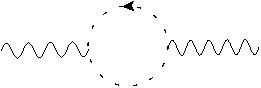
\includegraphics[scale=0.4]{1_loop_2_vert_CCA.jpg}
 \end{center}
\end{figure}

\noindent
En utilisant la même méthode, on obtient : 
\begin{eqnarray}
\Pi^{ab}_{\mu\nu}(p) &=& \frac{-i g^2 \delta^{ab}}{16 \pi^{2}} \left[
\left( g_{\mu\nu}p^2 - p_{\mu}p_{\nu} \right) \left( \frac{1}{6} \epsilon^{-1} + C_3 \right)
+ \frac{1}{2} p_{\mu} p_{\nu} ( C_4 + \frac{1}{\epsilon} ) \right.\\ 
    &+& \left. \left( g_{\mu \nu} p^2 - p_{\mu} p_{\nu} \right) \frac{1}{6} ln(\frac{\mu^2}{-p^2})
+\frac{1}{2} p_{\mu} p_{\nu}  ln( \frac{\mu^2}{- p^2} ) \right]
\end{eqnarray}

\noindent
\underline{\textbf{Tad pôle}}
\begin{figure}[H]
 \begin{center}
  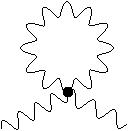
\includegraphics[scale=0.4]{1_loop_1_vert_3A.jpg}
 \end{center}
\end{figure}

\noindent
D'une part, par définition de la régularisation dimenssionelle, ce diagramme n'a pas de contribution, 
et d'autre part le calcul direct de l'amplitude de ce diagramme donne zéro. En effet ce diagramme fait intervenir le vertex $V_{A^{4}}$ 
(vertex à quatres lignes de champ de jauge), or pour ce diagramme ce vertex est nul. 
\begin{eqnarray}
 V_{A^{4}} &=& g^{2} \left[ f^{abe} f^{cde} \left( g_{\mu \rho}g_{\nu \rho} - g_{\mu \sigma}g_{\mu \rho} \right) \right. \nonumber  \\
&& + f^{ace} f^{bde} \left( g_{\mu \nu}g_{\rho \sigma} - g_{\mu \sigma}g_{\rho \nu} \right) \nonumber  \\
&& \left. +f^{ade} f^{cbe} \left( g_{\mu \rho}g_{\sigma \nu} - g_{\mu \nu}g_{\sigma \rho} \right) \right] .  
\end{eqnarray}
Or dans ce diagramme deux des lignes de ce vertex sont reliées. Prenons $\rho=\sigma$ et $c=d$.
\begin{eqnarray}
 V_{A^{4}} &=& g^{2} \left[ f^{abe} f^{dde} \left( g_{\mu \rho}g_{\nu \rho} - g_{\mu \rho}g_{\mu \rho} \right) \right. \nonumber  \\
&& + f^{ade} f^{bde} \left( g_{\mu \nu}g_{\rho \rho} - g_{\mu \rho}g_{\rho \nu} \right) \nonumber  \\
&& \left. +f^{ade} f^{dbe} \left( g_{\mu \rho}g_{\rho \nu} - g_{\mu \nu}g_{\rho \rho} \right) \right]  \\
           &=& 2 g^{2} f^{ade} f^{bde} \left[  g_{\mu \nu}g_{\rho \rho} - g_{\mu \rho}g_{\rho \nu} \right]  \\
           &=& 0 .
\end{eqnarray}

\noindent
\noindent
\underline{\textbf{Diagramme à une boucle}} \\
On a donc au final :
\begin{equation}
\Pi^{ab}_{\mu \nu}(p) = \frac{-i g^2 \delta^{ab}}{16 \pi^{2}} 
\left( g_{\mu\nu}p^2 - p_{\mu}p_{\nu} \right) 
\left[ \frac{10}{3} \epsilon^{-1} + C_5 + \frac{10}{3} ln(\frac{\mu^2}{-p^2})  \right]
\end{equation}
On a réussi par cette méthode à isoler la divergence. Le contre terme correspondant est donc :
\begin{eqnarray}
 (z_{2} - 1) &=& \frac{5g^2}{24 \pi^2} \epsilon^{-1}
\end{eqnarray}

\vspace{2cm}
\noindent
\underline{\textbf{Ensemble des contres-termes}}\\

$\bullet$\hspace{1mm}\textbf{Fonctions deux points}
\begin{eqnarray}
&&  (z_{2} - 1) =\frac{5g^2}{24 \pi^2} \epsilon^{-1} \\
&& \delta \mathcal{L}_{A^{2}} = (z_{2} - 1) \frac{1}{2} tr [ ( \partial_{\nu} A_{\mu} - \partial_{\mu} A_{\nu} )^2 ]
\end{eqnarray}

$\bullet$\hspace{1mm}\textbf{Fonctions trois points}
\begin{eqnarray}
&&  (z_{3} - 1) =\frac{g^3}{12 \pi^2} \epsilon^{-1} \\
&& \delta \mathcal{L}_{A^{3}} = (z_{3} - 1) (-g) tr [ ( \partial_{\nu} A_{\mu} - \partial_{\mu} A_{\nu} ) [A_{\mu},A_{\nu}] ]
\end{eqnarray}

$\bullet$\hspace{1mm}\textbf{Fonctions quatres points}
\begin{eqnarray}
&&  (z_{4} - 1) =\frac{-g^2}{24 \pi^2} \epsilon^{-1} \\
&& \delta \mathcal{L}_{A^{4}} = (z_{4} - 1) \frac{g^2}{2} tr [ [A_{\mu},A_{\nu}]^2  ]
\end{eqnarray}\\

$\bullet$\hspace{1mm}\textbf{Self énergie des fantômes}
\begin{eqnarray}
&&  (\tilde{z}_{2} - 1) =\frac{g^2}{24 \pi^2} \epsilon^{-1} \\
&& \delta \mathcal{L}_{\overline{c}c} =  (\tilde{z}_{2} - 1) \frac{1}{2} tr [ \overline{c} \Box c ]
\end{eqnarray}\\

$\bullet$\hspace{1mm}\textbf{Correction du troisième ordre en le vertex CCA}
\begin{eqnarray}
&&  (\tilde{z}_{3} - 1) =\frac{-g^2}{16 \pi^2} \epsilon^{-1} \\
&& \delta \mathcal{L}_{\overline{c}Ac} =  (\tilde{z}_{3} - 1) ( \frac{-1}{2} ) tr [ \overline{c} \partial_{\mu} [A_{\mu}, c] ]
\end{eqnarray}\\

\vspace{2cm}
\noindent
\underline{\textbf{Lagrangien renormalisé à une boucle}}\\
\begin{eqnarray}
\mathcal{L}_{R} &=& \mathcal{L} + \delta \mathcal{L}_{A^2} +  \delta \mathcal{L}_{A^3} +  \delta \mathcal{L}_{A^4}  
+  \delta \mathcal{L}_{\overline{c}c}  + \delta \mathcal{L}_{\overline{c}Ac}  \\
                              &=&  \frac{1}{2} tr[ \frac{1}{4} [ ( \partial_{\nu]}A_{\mu}- \partial_{\mu]}A_{\nu} ) 
+ g [A_{\mu},A_{\nu}] ]^2 
- \frac{1}{2 \alpha} (\partial_{\mu} A_{\mu} )^2 - \overline{c} ( \Box c - g \partial_{\mu}c - g\partial_{\mu} [A_{\mu},c]) ]  \nonumber  \\
                              &+& \frac{1}{8} (z_{2} - 1) \frac{1}{2} tr [ ( \partial_{\nu} A_{\mu} - \partial_{\mu} A_{\nu} )^2 ] \nonumber \\
                              &+& \frac{1}{4} g  (z_{3} - 1) (-g) 
tr [ ( \partial_{\nu} A_{\mu} - \partial_{\mu} A_{\nu} ) [A_{\mu},A_{\nu}] ] \nonumber \\
                              &+& \frac{1}{8} g^2 (z_{4} - 1) \frac{g^2}{2} tr [ [A_{\mu},A_{\nu}]^2  ] \nonumber \\
                              &-& \frac{1}{2} (\tilde{z}_{2} - 1) \frac{g^{2}}{2}  \epsilon^{-1} tr [ \overline{c} \Box c ] \nonumber \\
                              &+& \frac{1}{2}  (\tilde{z}_{3} - 1) ( \frac{-1}{2} ) tr [ \overline{c} \partial_{\mu} [A_{\mu}, c] ].
\end{eqnarray}
Ce que l'on peut encore écrire comme :
\begin{eqnarray}
\mathcal{L}_{R} &=& \frac{1}{2} tr\left[ \frac{1}{4} z_{2} \left( ( \partial_{\nu}A_{\mu}- \partial_{\mu}A_{\nu} )^2 
+ \frac{g}{2} z_{3} 
( \partial_{\nu]}A_{\mu}- \partial_{\mu]}A_{\nu} ) [A_{\mu},A_{\nu}]  - \frac{g^2}{4} z_{2}^{-1}  z_{4}[A_{\mu},A_{\nu}] ^2 \right) \right. \nonumber \\
  &&\left.  - \frac{1}{2 \alpha} 
(\partial_{\mu} A_{\mu} )^2 - \tilde{z}_{2} \left(\overline{c} \Box c - \tilde{z}_{2}^{-1} \tilde{z}_{3} g \overline{c} \partial_{\mu} [A_{\mu},c] \right). \right]
\end{eqnarray}
On définit les champs et les paramètres renormalisés comme suit :
\begin{eqnarray}
 && A_{0} = z_{2}^{\frac{1}{2}} A  \\
 && c_{0} = \tilde{z}_{2}^{\frac{1}{2}} c  \\
 && \overline{c}_{0} = \tilde{z}_{2}^{\frac{1}{2}} \overline{c} \\
 && g_{0} = z_{3}z_{2}^{\frac{3}{2}} g \\
 && \alpha_{0} = z_{2} \alpha
\end{eqnarray}
On s'aperçoit qu'en renormalisant on a modifié les coefficients mais on a pas toucher aux opérateurs, qui eux restent les mêmes. 
En fait ce que l'on mesure ce sont sont ces coefficients renormalisés, ceci traduit l'action des interactions mise en jeu entre 
les particules. 

%%%%%%%%%%%%%%%%%%%%%%%%%%%%%%%%%%%%%%%%%%%%%%%%%%%%%%%%%%%%%%%%%%%%%%%%%%%%%%%%%%%%%%%%%%%%%%%%%%%%%%%%%%%%%%%%%%%%%%%%%%%%%%%%%%
\subsection{Preuve de la renormalisabilité à tout les ordres}
%%%%%%%%%%%%%%%%%%%%%%%%%%%%%%%%%%%%%%%%%%%%%%%%%%%%%%%%%%%%%%%%%%%%%%%%%%%%%%%%%%%%%%%%%%%%%%%%%%%%%%%%%%%%%%%%%%%%%%%%%%%%%%%%%%


\noindent
On peut develloper les fonctions de correlations $\Gamma$ en serie de puissance de $\hbar$. On écrit :
\begin{eqnarray}
 \Gamma = \Gamma^{0} + \Gamma^{1} + \Gamma^{2} + ...
\end{eqnarray}
En particulier : 
\begin{eqnarray}
 \Gamma = \Gamma_{R}^{n} + \Gamma^{n}_{div}
\end{eqnarray}
On pose :
\begin{eqnarray}
 \Gamma_1 * \Gamma_2 = \int dx \left( \frac{\delta \Gamma_{1}}{\delta A} \frac{\delta \Gamma_{2}}{\delta k} 
+ \frac{\delta \Gamma_{1}}{\delta c} \frac{\delta \Gamma_{2}}{\delta l} \right)
\end{eqnarray}
Les Identité de Slavnov  s'écrivent avec cette notation de la façon suivante :
\begin{eqnarray}
 \sum_{p=0}^{n} \Gamma^{(p)} * \Gamma^{(n-p)} = 0
\end{eqnarray}

\noindent
$\bullet$ \textit{Commençons par le cas $n=0$ :}
\begin{eqnarray}
 && \Gamma^{0} = \int dx \left[ \mathcal{L}_{eff} + k^{\mu}_{a} s A^{a}_{\mu} - l^{a} s c^{a} \right] := I\\
 && I*I = 0
\end{eqnarray}
Démontrer cette relation est évident. \\

\noindent
$\bullet$\textit{Étudions à présent le cas $n=1$ :}
\begin{equation}
 \sum_{p=0}^{1} \Gamma^{(p)} * \Gamma^{(n-p)} = 0 = \Gamma^{0} \Gamma^{1} + \Gamma^{1} * \Gamma^{0}
\end{equation}
ce qui nous permet d'écrire :
\begin{eqnarray*}
 && I * \Gamma^{1}_{R} + \Gamma^{1}_{R} * I = 0 \hspace{2mm} \rightarrow \hspace{2mm} \text{Cette relation est bien vérifiée !} \\
 && I * \Gamma^{1}_{div} + \Gamma^{1}_{div} * I = 0 \hspace{2mm} \rightarrow \hspace{2mm} \text{On veut que cette relation soit 
vérifiée.}
\end{eqnarray*}
On a envie d'écrire une action $I_{1}$ tel que :
\begin{equation}
I_{1} = I - \Gamma^{1}_ {div}
\end{equation}
On deva avoir :
\begin{equation}
 I_{1} * I_{1} = 0.
\end{equation}
Or $I_{1}$ est l'action renormalisée à l'ordre 1, et on a déjà calculé les contres termes à cet ordre. On a donc :
\begin{equation}
 I_{1} \left( A, c, \overline{c}, k, l \right) = I \left( A_{0}, c_{0}, \overline{c}_{0}, k_{0}, l_{0} \right)
\end{equation}
avec :
\begin{eqnarray}
 && A_{0} = z_{2}^{\frac{1}{2}} A  \\
 && c_{0} = \tilde{z}_{2}^{\frac{1}{2}} c  \\
 && \overline{c}_{0} = \tilde{z}_{2}^{\frac{1}{2}} \overline{c} \\
 && k_{0} = \tilde{z}_{2}^{\frac{1}{2}} k \\
 && l_{0} = z_{4} l
\end{eqnarray}
on a alors :
\begin{equation}
 I_{1} * I_{1} = \int dx \left[ z_{2}^{\frac{1}{2}} \tilde{z}_{2}^{\frac{1}{2}} \frac{\delta I_{1}}{\delta A_{0}} \frac{\delta I_{1}}{\delta k_{0}}
+ \tilde{z}_{2}^{\frac{1}{2}} z_{4} \frac{\delta I_{1}}{\delta c_{0}}\frac{\delta I_{1}}{\delta l_{0}} \right]
\end{equation}
Le fait d'avoir $I_{1} * I_{1} = 0$ nous donne une realtion entre les coefficient de renormalisation $z_{i}$.
\begin{equation}
 I_{1} * I_{1} = 0 \Leftrightarrow z_{2}^{\frac{1}{2}} \tilde{z}_{2}^{\frac{1}{2}} = \tilde{z}_{2}^{\frac{1}{2}} z_{4}
\end{equation}

\noindent
$\bullet$ \textit{Plaçons nous à présent dans le cas $n$ quelconque :}  \\
On a alors :
\begin{eqnarray}
 &&\sum_{p=0}^{n} \Gamma^{(p)} * \Gamma^{(n-p)} = 0 = \Gamma^{(0)} * \Gamma^{(n)} + \sum_{p=1}^{n-1} \Gamma^{(p)} * \Gamma^{(n-p)} 
+ \Gamma^{(n)} * \Gamma^{(0)}\\
 &&\Gamma^{(0)} * \Gamma^{(n)} + \Gamma^{(n)} * \Gamma^{(0)} = -\sum_{p=1}^{n-1} \Gamma^{(p)} * \Gamma^{(n-p)} \\
\end{eqnarray}
or le terme $ \sum_{p=1}^{n-1} \Gamma^{(p)} * \Gamma^{(n-p)}$ est fini par hypothèse de recurrence.\\
On a alors : 
\begin{equation}
 I * \Gamma^{(n)} + \Gamma^{(n)} * I = 0
\end{equation}
ce qui nous permet d'écrire une nouvelle fois :
\begin{eqnarray}
  && I * \Gamma^{(n)}_{R} + \Gamma^{(n)}_{R} * I = 0   \\
  && I * \Gamma^{(n)}_{div} + \Gamma^{(n)}_{div} * I = 0
\end{eqnarray}
Pour la suite on défint un opérateur $\sigma$ tel que :
\begin{equation}
 \sigma \Gamma^{n}_{div} := I * \Gamma^{n}_{div} + \Gamma^{n}_{div} * I = 0
\end{equation}
En posant :
\begin{equation}
 \left(x_{i}\right) = \left(A,c\right) \text{ \hspace{5mm} et \hspace{5mm} }  \left(\theta_{i}\right) = \left(k,l\right)
\end{equation}
on peut définir $\sigma$ comme suit :
\begin{equation}
 \sigma := \frac{\partial I}{\partial x_{i}} \frac{\partial}{\partial \theta_{i}} + 
\frac{\partial I}{\partial \theta_{i}} \frac{\partial}{\partial x_{i}}
\end{equation}
\underline{Remarque :}\\
Il est interessant de noter que l'on a :
\begin{eqnarray}
 && \frac{\partial I}{\partial x_{i}} \frac{\partial I}{\partial \theta_{i}} = 0 \\
 && \frac{\partial \Gamma}{\partial x_{i}} \frac{\partial \Gamma}{\partial \theta_{i}} = 0
\end{eqnarray}\\

\noindent
L'opérateur $\sigma$ ainsi définie vérifie $\sigma^{2}=0$. En effet à partir de la définition de $\sigma$ on peut écrire :
\begin{eqnarray*}
 \sigma^2 &=& \left( \frac{\partial I}{\partial x_{i}} \frac{\partial}{\partial \theta_{i}} + 
\frac{\partial I}{\partial \theta_{i}} \frac{\partial}{\partial x_{i}} \right)
\left( \frac{\partial I}{\partial x_{j}} \frac{\partial}{\partial \theta_{j}}  + 
\frac{\partial I}{\partial \theta_{j}} \frac{\partial}{\partial x_{j}} \right)\\
          &=& \frac{\partial I}{\partial x_{i}} \frac{\partial}{\partial \theta_{i}} 
\left( \frac{\partial I}{\partial x_{j}} \frac{\partial}{\partial \theta_{j}} \right) 
    + \frac{\partial I}{\partial x_{i}} \frac{\partial}{\partial \theta_{i}} 
\left( \frac{\partial I}{\partial \theta_{j}} \frac{\partial}{\partial x_{j}} \right)
    + \frac{\partial I}{\partial \theta_{i}} \frac{\partial}{\partial x_{i}} 
\left( \frac{\partial I}{\partial x_{j}} \frac{\partial}{\partial \theta_{j}} \right)
    + \frac{\partial I}{\partial \theta_{i}} \frac{\partial}{\partial x_{i}} 
\left( \frac{\partial I}{\partial \theta_{j}} \frac{\partial}{\partial x_{j}} \right)\\
          &=& \frac{\partial I}{\partial x_{i}} \frac{\partial I}{\partial x_{j}}  
\left( \frac{\partial }{\partial \theta_{i}} \frac{\partial}{\partial \theta_{j}} \right)  
    + \frac{\partial I}{\partial x_{i}} \frac{\partial}{\partial \theta_{j}} 
\left( \frac{\partial }{\partial \theta_{i}} \frac{\partial}{\partial x_{j}} \right)
    + \frac{\partial I}{\partial \theta_{i}} \frac{\partial}{\partial x_{j}} 
\left( \frac{\partial }{\partial x_{i}} \frac{\partial}{\partial \theta_{j}} \right)
    + \frac{\partial I}{\partial \theta_{i}} \frac{\partial}{\partial \theta_{j}} 
\left( \frac{\partial }{\partial x_{i}} \frac{\partial}{\partial x_{j}} \right)\\
    && + \frac{\partial I}{\partial x_{i}} \frac{\partial I}{\partial \theta_{i} \partial x_{j}} 
\frac{\partial}{\partial \theta_{i}}
    + \frac{\partial I}{\partial x_{i}} \frac{\partial I}{\partial \theta_{i} \theta_{j}}
\frac{\partial}{\partial x_{j}}
    + \frac{\partial I}{\partial \theta_{i}} \frac{\partial I}{\partial x_{i} x_{j}}
\frac{\partial}{\partial \theta_{j}}
    + \frac{\partial I}{\partial \theta_{i}} \frac{\partial I}{\partial x_{i} \partial \theta_{j}}
\frac{\partial}{\partial x_{j}} \\
\end{eqnarray*}
Les termes de la premiere ligne sont nuls un à un, car chaccun des termes est le produit d'une entité symétrique avec une entité antisymétrique.
Les termes de la dernieres lignes sonts nuls à cause du fait que l'on ait : 
\begin{equation}
 \frac{\partial I}{\partial \theta_{i} \partial x_{i}} = 0
\end{equation}
On a donc bien $\sigma^{2}=0$\\

\noindent
On se rappelle que l'on a :
\begin{eqnarray*}
 \mathcal{I} &=&  \int \left[
\frac{-1}{4g} F^{a}_{\mu\nu}(x)F^{a}_{\mu \nu}(x) 
+ \frac{1}{\alpha}(\partial_{\mu}A_{\mu}^{a})^2 .
+ \overline{c}^{a}(x)M^{ab}c^{b}(x) 
+ k_{\mu}^{a} D_{\mu}c^{a} 
+ \frac{1}{2}f^{abd}l^ac^bc^d \right]
\end{eqnarray*} 

\noindent
On va vouloir écrire $\cal{I}_{n} = \cal{I}_{n-1} - \Gamma_{div}^{n}$. Par une analyse dimensionnelle et avec les identités de Slavnov, 
matérialisé avec l'opérateur $\sigma$, on va pouvoir écrire $\Gamma_{div}^{n}$. 

\noindent
\underline{Analyse dimensionelle}
\begin{eqnarray*}
 && \text{degré en fantômes :}\\
 && g(c) := 1 \hspace{3mm} \text{et} \hspace{3mm} g(\overline{c}):=-1 \\
 \text{donc, } && g(k) = -1 \hspace{3mm} \textit{et} \hspace{3mm} g(l)=-2\\
&& \vspace{3mm} \\
 &&\text{degré en champs :} \\
 && d(A) := 1 \hspace{3mm} \text{et} \hspace{3mm} d(\partial A):=2 \\
\text{donc, }  && d(FF)=4\\
 && d( (\partial A)^{2}) = 4\\
 && d(M) = 2  \hspace{3mm} \text{et} \hspace{3mm} d(\overline{c}) + d(c) =2 \hspace{3mm}  \rightarrow d(\overline{c}) := d(c) = 1 \\
 && d(D) =1  \hspace{3mm} \textit{et} \hspace{3mm} d(k) = 2 \\
 &&  d(l) = 2
\end{eqnarray*}
On peut alors écrire :
\begin{eqnarray}
 \Gamma^{n}_{div} &=& \int dx \left[  L(A) +  \left(  \overline{c}^{a} \partial_{\mu}  + k_{\mu}^{b} \right) \Delta_{mu} c^{b} 
+ \frac{\gamma}{2} f^{abd} l^{a}c^{b}c^{d} \right]
\end{eqnarray}
Par analyse dimenssionnelle on peut déjà en déduire :
\begin{eqnarray}
 && d(\Delta) = 1 \hspace{3mm} \text{et} \hspace{3mm}  g(\Delta) = 0 \\
 && \text{donc,} \hspace{3mm} \Delta_{\mu} = \alpha \partial_{\mu} +\beta f^{abd} A^{d}_{\mu}
\end{eqnarray}
on peut alors calculer :
\begin{eqnarray}
 \sigma \Gamma^{n}_{div} = 0 \Leftrightarrow  
D_{\mu} \frac{\partial L}{\partial A_{\mu}} + (\beta-\alpha) f^{abd} A^{b}_{\mu}  \frac{\partial \mathcal{L}}{\partial A_{\mu}} = 0
\end{eqnarray}
dont la solution est :
\begin{eqnarray}
 L &=& a \mathcal{L} + (\beta - \alpha) A \frac{\mathcal{L}}{A}
\end{eqnarray}
On a onc au final :
\begin{eqnarray}
 \Gamma^{n}_{div} &=& \int dx \left[  \lambda \mathcal{L} + (\beta - \alpha) A \frac{\mathcal{L}}{A} 
+ \alpha ( \overline{c}  \partial + k) \Delta c + (\beta - \alpha) ( \overline{c}  \partial + k)f^{abd} A^{d}c^b 
+ \frac{\beta}{2} f^{abd} l^{a}c^{b}c^{d} \right] \nonumber \\
                  &=& \left[ \int dx \left( ( \beta - \alpha + \frac{a}{2}) \left[A \frac{\delta}{\delta A} 
+ l \frac{\delta}{\delta l} \right] + \frac{\alpha}{2} \left[k \frac{\delta}{\delta k} + c \frac{\delta}{\delta c} 
+ \overline{c} \frac{\delta}{\delta  \overline{c} } \right]  \right) - \frac{\lambda}{2} g \frac{\delta}{\delta g}    \right] \mathcal{I}
\end{eqnarray}

\noindent
Or par hypothèse de récurence on a : 
\begin{eqnarray}
 \mathcal{I}_{n-1} &=& \mathcal{I} \left( z_{2,n-1}^{\frac{1}{2}}A , \tilde{z}^{\frac{1}{2}}_{2,n-1}c, 
\tilde{z}^{\frac{1}{2}}_{2,n-1} \overline{c} , \tilde{z}^{\frac{1}{2}}_{2,n-1}k , z_{4,n-1} l, z_{g,n-1} g  \right),
\end{eqnarray}
ce qui nous permet d'écrire :
\begin{eqnarray}
 && z_{2,n}^{\frac{1}{2}} = z_{2,n-1}^{\frac{1}{2}} - \left( \beta - \alpha + \frac{a}{2} \right)\\
 && \tilde{z}_{2,n}^{\frac{1}{2}} = \tilde{z}_{2,n-1}^{\frac{1}{2}} - \left( \frac{\alpha}{2}\right) \\
 && z_{g,n}^{\frac{1}{2}} = z_{g,n-1}^{\frac{1}{2}} - \left( \frac{\lambda}{2}\right)
\end{eqnarray}

\noindent
On a donc montré qu'à chaque ordre on a un nombre finis de contre termes. Ce qui achève la démonstration de la renormalisabilité de la théorie
à tout les ordres.  

%%%%%%%%%%%%%%%\frametitle{Preuve de la renormalisabilité à tout les ordres}%%%%%%%%%%%%%%%%%%%%%%%%%%%%%%%%%%%%%%%%%%%%%%%%%%%%%%%%%%%%%%%%%%%%%%%%%%%%%%%%%%%%%%%%%%%%%%%%%%%%%%%%%%%%%%%%%%%
\section{Apparté Non Commutative}
%%%%%%%%%%%%%%%%%%%%%%%%%%%%%%%%%%%%%%%%%%%%%%%%%%%%%%%%%%%%%%%%%%%%%%%%%%%%%%%%%%%%%%%%%%%%%%%%%%%%%%%%%%%%%%%%%%%%%%%%%%%%%%%%%%


%%%%%%%%%%%%%%%%%%%%%%%%%%%%%%%%%%%%%%%%%%%%%%%%%%%%%%%%%%%%%%%%%%%%%%%%%%%%%%%%%%%%%%%%%%%%%%%%%%%%%%%%%%%%%%%%%%%%%%%%%%%%%%%%%%
\subsection{Algèbre de Moyal et théorie de jauge}
%%%%%%%%%%%%%%%%%%%%%%%%%%%%%%%%%%%%%%%%%%%%%%%%%%%%%%%%%%%%%%%%%%%%%%%%%%%%%%%%%%%%%%%%%%%%%%%%%%%%%%%%%%%%%%%%%%%%%%%%%%%%%%%%%%

\noindent
Nous allons dans cette partie introduire les notions d'espace de Moyal, et de théorie de jauge sur ce même espace. Nous renvoyons le lecteur en 
annexe, pour des compléments en mathématique.\\

\noindent
L'espace de Moyal est une déformation de l'espace euclidien. Sans rentrer dans des détails mathématique, nous pouvons dire que le produit habituel 
est remplacé par le produit de Moyal, qui agit entre des éléments de $\cal{S}$($\mathbb{R}^{D}$), epace des fonctions Schwartz de $\mathbb{R}^{D}$.
\begin{eqnarray}
 \forall a,b \in \mathcal{S} , \hspace{1cm}  (a \star b) (x)  = \frac{1}{(\pi \theta)^{D}}  \int  d^{D}y    d^{D}z   a(x+y)   b(x+z)   
e^{-i y \tilde{z} }
\end{eqnarray}
où,
\begin{eqnarray}
 &\bullet&  \tilde{z}_{\nu}  =  2 \Theta^{-1}_{\mu \nu} z_{\nu}  \\
 &\bullet&  y \tilde{z} = y_{\mu}  \tilde{z}_{\nu}  \\
 &\bullet&  \Theta_{\mu \nu}  =  \theta  \text{diag ( J,..., J) , une matrice} \hspace{2mm} D \times D  \\
 &\bullet&  J = 
\left(
  \begin{array}{ c c }
     0 & -1 \\
     1 & 0
  \end{array} 
\right)
\end{eqnarray}

\noindent
Nous définissons l'algèbre de Moyal, noté $\cal{M}$, comme suit :
\begin{center}
 $\mathcal{M}  =  \left \{ \right. T \in \mathcal{S}'(\mathbb{R}^{D})$ ,  $\forall \in \mathcal{S}$ /  ($T \star  a) \in \mathcal{S}$   
et $(a \star  T) \in \mathcal{S} \left.  \right \}$
\end{center}
où  $\mathcal{S}'(\mathbb{R}^{D})$ est l'espace des distributions tempéré de $\mathbb{R}^{D}$.\\

\noindent
Nous donnons quelques proriétés importantes, $\forall a,b \in \mathcal{M}$,
\begin{eqnarray}
 &\bullet& (a \star b )^{\dagger}  b^{\dagger}  \star  a^{\dagger}  \\
 &\bullet& \partial_{\mu} (a \star b) = (\partial_{\mu}a) \star b  +  a \star  (\partial_{\mu} b) \\
 &\bullet& \int d^{D}x (a\star b) = \int d^{D}x a.b \\
 &\bullet& [ \tilde{x}_{\mu} ,a ]_{\star} = 2i ( \partial_{\mu} a)
\end{eqnarray}

\noindent
Comme nous le savons, dans la théorie de Yang Mills, les champs sont des potentiels de jauge, associé à des connexions. Il est possible de 
définir la notion de connexion sur l'espace de Moyal.
\begin{eqnarray}
 \forall \Phi, \hspace{2mm}  \nabla_{\mu} \Phi :=   \nabla_{\partial_{\mu}} \Phi  = \partial_{\mu} \Phi - iA_{\mu} \star  \Phi
\end{eqnarray}
où  $A_{\mu} := i \nabla_{\mu}(1)$.\\

\noindent
La courbure de $\nabla$ est donnée par l'application linéaire suivante :
\begin{eqnarray}
 F_{\mu \nu}  &:=&  [ \nabla_{\partial_{\mu}}  , \nabla_{\partial_{\nu}}  ] - \nabla_{[ \partial_{\mu} , \partial_{\nu} ]}   \\
                        &=&  - i ( \partial_{\mu} A_{\nu}  -   \partial_{\nu} A_{\mu}  - i [ A_{\mu} , A_{\mu} ]_{\star}  )
\end{eqnarray}

\noindent
Nous notons $\cal{U}(\cal{M})$ les éléments unitaires de $\cal{M}$. Il est alors possible de montrer que l'on a, $\forall g \in \cal{U}(\cal{M})$ :
\begin{eqnarray}
 && A_{\mu}^{g} = g \star A_{\mu} \star g^{\dagger} + ig \star ( \partial_{\mu} g^{\dagger} )  \\
 && F_{\mu \nu }^{g} = g \star F_{\mu \nu}  \star   g^{\dagger}
\end{eqnarray}

\noindent
Lorsque l'on calcule $A_{\mu}^{g}$, en écrivant $ \partial_{\mu} g^{\dagger}  =  [ i \tilde{x}_{\mu} , g^{\dagger}   ]_{\star}$, on s'aperçoit 
que l'on construit un autre champ, dont sa trace est invariante de jauge.
\begin{eqnarray}
  A_{\mu}^{g}  &=&  g \star A_{\mu} \star g^{\dagger} + i g \star  [ i \tilde{x}_{\mu} , g ]_{\star}   \\
                         &=&  g \star A_{\mu} \star g^{\dagger} - g \star  \tilde{x}_{\mu} \star  g  + g \star  g^{\dagger}     \\
                         &=&  g \star \left(  A_{\mu} -  \tilde{x}_{\mu} \right) \star  g
\end{eqnarray}
Et si on pose $\cal{A}_{\mu}  =  A_{\mu} - $ $ \tilde{x}_{\mu}  $, on montre facilement que $g \star \cal{A}_{\mu}  \star$  $g^{\dagger}$

%%%%%%%%%%%%%%%%%%%%%%%%%%%%%%%%%%%%%%%%%%%%%%%%%%%%%%%%%%%%%%%%%%%%%%%%%%%%%%%%%%%%%%%%%%%%%%%%%%%%%%%%%%%%%%%%%%%%%%%%%%%%%%%%%%
\subsection{Theorie de yang Mills Non Commutative sur le plan de Moyal}
%%%%%%%%%%%%%%%%%%%%%%%%%%%%%%%%%%%%%%%%%%%%%%%%%%%%%%%%%%%%%%%%%%%%%%%%%%%%%%%%%%%%%%%%%%%%%%%%%%%%%%%%%%%%%%%%%%%%%%%%%%%%%%%%%%

\noindent
On va se placer sur le plan de Moyal ($D=2$). Et nous considererons comme groupes de structure U(1) et SU(N).
\noindent
Nous allons calculer la fonction deux points en les fantômes. On notera par des lettres majuscule $(A,B,C,...)$ les indices de $U(N)$, 
et par des lettres minuscule $(a,b,c,...)$ les indices de $SU(N)$. Nous travaillerons en dimension $D=2$.\\

\noindent
J'ai admis l'expression de l'action de jauge noncommutative $U(N)$.
\begin{eqnarray}
 \cal{I}  &=&  \int d^{2 } x  \left(  \frac{1}{4}  F_{\mu  \nu}  \star  F_{\mu  \nu}  + s \left( \overline{c} \star \partial_{\mu} A_{\mu}   
+  \frac{\alpha}{2} \overline{c} \star b \right)  \right)
\end{eqnarray}
avec les notations BRST suivante :
\begin{eqnarray}
 &&s A_{\mu}  = D_ {\mu} c,  \\
 &&s \overline{c} = b,  \\
 &&s c = i g c\star c,  \\
 &&sb = 0,\\
 &&s^{2} = 0.
\end{eqnarray}\\

\noindent
De la même façon que sur Minkowski, on arrive à obtenir les règles de Feynman.\\
\textbf{Règles de feynman}\\

\begin{itemize}
 \renewcommand{\labelitemi}{$\bullet$}

 \item Propagateur en les champs de jauge $A_{\mu}$
\begin{eqnarray}
 G^{ A^{A} B^{B} } (k)  &=&  \frac{ \delta^{AB} }{ k^2 } \left(  \delta_{\mu \nu}  - (1-\alpha)  \frac{ k_{\mu} k_{\nu} }{ k^2 } \right) 
\end{eqnarray}
Pour la suite du calcul, nous considererons la jauge de Feynman  $\alpha=1$.
\item Propagateur en les fantomes
\begin{eqnarray}
 G^{ \overline{c}^{A} c^{B} } (k)  &=& - \frac{ \delta^{AB} }{ k^2 } 
\end{eqnarray}

\item Vertex 2 branches fantomes et une champ de jauge
\begin{eqnarray}
 V_{\mu}^{ \overline{c}^{0} A^{A} c^{B} } (q_1 , k_2 , q_3 ) &=& -2ig (2 \pi)^2 \delta^{2} ( q_1 +k_2 +q_3 ) q_{3_{\mu}} \frac{d^{AB0}}{2} 
sin( \frac{\epsilon}{2}  q_1 \tilde{q}_3 ) \\
 V_{\mu}^{ \overline{c}^{a} A^{b} c^{c} } (q_1 , k_2 , q_3 ) &=& -2ig (2 \pi)^2 \delta^{2} ( q_1 +k_2 +q_3 ) q_{3_{\mu}} \mathcal{F}^{acb}(q_1 , q_3)
\end{eqnarray}

\item Vertex 3 branches en champ de jauge
\begin{eqnarray*}
 V_{\rho  \sigma  \tau}^{ A^{A} A^{B} c^{0} } (k_1 , k_2 , k_3 ) &=&  2ig (2 \pi)^2 \delta^{2} ( k_1 + k_2 + k_3 )  \mathcal{F}^{AB0}(k_1 , k_2) \\
&&   \left[
(k_3  -  k_2)_{\rho}  \delta_{\sigma  \tau}  +  (k_1  -  k_3)_{\sigma}  \delta_{\rho  \tau}  +  (k_2  -  k_1)_{\tau}  \delta_{\rho  \sigma }
\right]      \\
  V_{\rho  \sigma  \tau}^{A^{a} A^{b} c^{d} } (k_1 , k_2 , k_3 ) &=& 2ig (2 \pi)^2 \delta^{2} ( k_1 + k_2 + k_3 )  \mathcal{F}^{abc}(k_1 , k_2)  \\
&&   \left[
(k_3  -  k_2)_{\rho}  \delta_{\sigma  \tau}  +  (k_1  -  k_3)_{\sigma}  \delta_{\rho  \tau}  +  (k_2  -  k_1)_{\tau}  \delta_{\rho  \sigma }
\right]
\end{eqnarray*}

avec,
\begin{eqnarray}
 \mathcal{F}^{abc}(q_1 , q_3)  &=&  \frac{d^{abc}}{2}   sin \left(  \frac{\epsilon}{2}  q_1  \tilde{q}_3  \right)   +    \frac{f^{abc}}{2}   cos \left(  \frac{\epsilon}{2}  q_1  \tilde{q}_3   \right)   \\
 \mathcal{F}^{abc}(q_1 , q_3)  &=&  \frac{d^{AB0}}{2}   sin \left(  \frac{\epsilon}{2}  q_1  \tilde{q}_3  \right)  \\
 \mathcal{F}^{a00}(q_1 , q_3)  &=& 0
\end{eqnarray}

\end{itemize}

\noindent
\underline{Formulaire}
\begin{eqnarray*}
 &\textbf{1.}& \frac{1}{k^2 (k+p)^2 }  =  \int_{0}^{1}   dx  \frac{1}{ \left[ (k+p(1-x))^2  +  p^2 x(1-x) \right]^2  }  \\
 &\textbf{2.}&  \int  \frac{d^D k}{(2 \pi)^D}   \frac{1}{\left[ k^2 + M^2 \right]^2 }  =  \frac{ \pi^{\frac{D}{2}} }{ (2 \pi)^{D}  }  (M^2)^{\frac{D}{2}-2} \Gamma(2-\frac{D}{2}) \\
 &\textbf{3.}& \int  \frac{d^D k}{(2 \pi)^D}   \frac{e^{ik \epsilon \tilde{p}}}{(\left[ k^2 + M^2 \right]^2 }  =   \frac{1}{2 (2 \pi )^{ \frac{D}{2}}}  M^{\frac{D}{2} - 2}  \left( \epsilon \left| \tilde{p}  \right|  \right)^{ 2-\frac{D}{2} }   \textbf{K}_{2- \frac{D}{2}  } ( M  \epsilon \left| \tilde{p}  \right|  )   \\
&\textbf{4.}&  f^{ade} f^{bde}  =  N  \delta^{ab}  \\
&\textbf{5.}&  d^{ade} d^{bde}  =  \left( N - \frac{4}{N} \right)  \delta^{ab}  \\
&\textbf{6.}&  d^{AB0} = \sqrt{\frac{2}{N}}  \delta^{ab}  \\
\end{eqnarray*}

%%%%%%%%%%%%%%%%%%%%%%%%%%%%%%%%%%%%%%%%%%%%%%%%%%%%%%%%%%%%%%%%%%%%%%%%%%%%%%%%%%%%%%%%%%%%%%%%%%%%%%%%%%%%%%%%%%%%%%%%%%%%%%%%%%
\subsubsection{Diagramme 1 boucle avec deux lignes externe en fantôme}
%%%%%%%%%%%%%%%%%%%%%%%%%%%%%%%%%%%%%%%%%%%%%%%%%%%%%%%%%%%%%%%%%%%%%%%%%%%%%%%%%%%%%%%%%%%%%%%%%%%%%%%%%%%%%%%%%%%%%%%%%%%%%%%%%%

\noindent
On s'interesse aux diagrammes $\overline{c}^{A}  -  c^{B}$. Étant donné que $A$ et $B$ sont égaux respectivement à $(0,a)$ et $(0,b)$, quatre possibilités s'offrent à nous.
 \begin{itemize}
 \renewcommand{\labelitemi}{$\checkmark$}

 \item $\overline{c}^{0}  -  c^{0}$, les deux vertex sont de type  $V_{\mu}^{ \overline{c}^{0} A^{A} c^{B} }$. \\
Le fateur algébrique est ici :
\begin{eqnarray}
 d^{B00} d^{A00} \delta^{AB} = \delta^{B0}  \delta^{A0}  \delta^{AB} =  \delta^{00}  =  1
\end{eqnarray}

 \item $\overline{c}^{0}  -  c^{b}$, les deux vertex sont soit les deux de type $V_{\mu}^{ \overline{c}^{0} A^{A} c^{B} }$, soit un $V_{\mu}^{ \overline{c}^{0} A^{A} c^{B} }$ et l'autre $V_{\mu}^{ \overline{c}^{a} A^{b} c^{c} }$ . \\ 
Dans chacun des cas le facteur algébrique est respectivement :
\begin{eqnarray}
 &1.&  d^{EB0} d^{A00} \delta^{AE} \approx \delta^{0b}  = 0  \\
 &2.&  d^{ae0} \mathcal{F}^{fbd} \delta^{ad} \delta^{ef} = d^{ae0} \mathcal{F}^{eba}  \approx d^{ae0} d^{eba} = \delta^{b0}  =  0
\end{eqnarray}


 \item $\overline{c}^{a}  -  c^{0}$. \\
Avec les vertex précedement établie, ce diagramme est impossible.

 \item et $\overline{c}^{a}  -  c^{b}$, les deux vertex sont de type  $V_{\mu}^{ \overline{c}^{a} A^{b} c^{c} }$. \\
Le fateur algébrique est ici :
\begin{eqnarray}
 \mathcal{F}^{ebd} \mathcal{F}^{aed} &\approx& d^{ebd} d^{aed} + f^{ebd} f^{aed} \\
                                                                   &\approx& \delta^{ab}
\end{eqnarray}

\end{itemize} 



$\bullet$ \textbf{ Diagramme 0-0 }
 \begin{eqnarray*}
 \omega_{00}(p) &=&  \int  \frac{d^D k}{(2 \pi)^D}
V_{\nu}^{ \overline{c}^{0} A^{B} c^{0} } (p-k , k , -p )
V_{\mu}^{ \overline{c}^{0} A^{A} c^{0} } (p,-k,k-p )
G^{ \overline{c}^{0} c^{0} } (k-p)
G^{ A^{A} A^{B} }_{\mu \nu } (k)  \\
                              &=&  \int  \frac{d^D k}{(2 \pi)^D}
( -2ig) (2 \pi)^2  (-p_{\nu} )  \frac{d^{B00}}{2} sin \left[ \frac{\epsilon}{2}  (p-k) (- \tilde{p} ) \right]            \\
&&        ( -2ig) (2 \pi)^2 (k-p)_{\mu}   \frac{d^{A00}}{2} sin \left[ \frac{\epsilon}{2}  p ( \tilde{k} - \tilde{p} ) \right]              \\
&&         \frac{-1}{(k-p)^2}
\frac{\delta^{AB} \delta^{\mu \nu}}{k^2}
\end{eqnarray*}
Le produit $p \tilde{p} $ est nul car $p \tilde{p} = p_{\mu} \theta_{\mu \nu} p_{\nu} $, et $\theta_{\mu \nu}$ est antisymétrique en $\mu$ et $\nu$. On va effetuer le changement de variable $k \rightarrow -k$. Nos utiliserons les relations 4, 5, et 6 du formulaire afin de déterminer completement le facteur algébrique, et également la realtion 1 de sorte à éliminer les termes linéaire en k ce afin de simplifier l'intégrales comme nous allons le voir.
\begin{eqnarray}
 \omega_{00}(p)  &=&  - g^2  (2 \pi)^4  2N^{-1}  \delta^{00}
\int  \frac{d^D k}{(2 \pi)^D}
\frac{pk + p^2}{k^2(k+p)^2}
sin^2 \left[ \frac{\epsilon}{2} k \tilde{p} \right]  \\
                              &=&  - g^2  (2 \pi)^4  2N^{-1}   \delta^{00}
\int_{0}^{1}  dx
\int  \frac{d^D k}{(2 \pi)^D}
\frac{(pk + p^2)  sin^2 \left[ \frac{\epsilon}{2} k \tilde{p} \right] }{\left[ (k+p(1-x))^2  +  p^2 x(1-x) \right]^2}  \\
                              &=&  - g^2  (2 \pi)^4  2N^{-1}    \delta^{00}
\int_{0}^{1}  dx
\int  \frac{d^D k}{(2 \pi)^D}
\frac{(pk + p^2 x)  sin^2 \left[ \frac{\epsilon}{2} k \tilde{p} \right] }{\left[ k^2  +  M^2 \right]^2}  \\
                              &=&  - g^2  (2 \pi)^4  2N^{-1}    \delta^{00} p^{2}
\int_{0}^{1}  dx x
\int  \frac{d^D k}{(2 \pi)^D}
\frac{sin^2 \left[ \frac{\epsilon}{2} k \tilde{p} \right] }{\left[ k^2  +  M^2 \right]^2}  
\end{eqnarray}
On pose,
\begin{eqnarray}
 I_{s} &=& \int  \frac{d^D k}{(2 \pi)^D}
\frac{sin^2 \left[ \frac{\epsilon}{2} k \tilde{p} \right] }{\left[ k^2  +  M^2  \right]^2}  \\
       &=&  \int  \frac{d^D k}{(2 \pi)^D}
\frac{1}{\left[ k^2  +  M^2 \right]^2} 
 \left( 1 - cos ( \epsilon k \tilde{p} ) \right) \\
                              &=&  \int  \frac{d^D k}{(2 \pi)^D}
\frac{1 }{\left[ k^2  +  M^2 \right]^2} 
 \left[ 1 - \frac{e^{ i \epsilon k \tilde{p} }   +   e^{i \epsilon k \tilde{p} } }{ 2 }  \right]
\end{eqnarray}
En utilisant les relations 2 et 3 du formulaire on parvient à écrire :
\begin{eqnarray}
 I_{s}  &=&  \frac{ \pi^{\frac{D}{2}} }{ (2 \pi)^{D}  }  (M^2)^{\frac{D}{2}-2} \Gamma(2-\frac{D}{2})
-  \frac{1}{2 (2 \pi )^{\frac{D}{2}}}  M^{\frac{D}{2} - 2}  \left( \epsilon \left| \tilde{p}  \right|  \right)^{ 2-\frac{D}{2} }   
\textbf{K}_{2- \frac{D}{2}  } ( M \epsilon  \left| \tilde{p}  \right|  )
\end{eqnarray}
Nous pouvons insérer ce résultat dans l'expression de $ \omega_{00}(p)$. 
\begin{eqnarray}
 \omega_{00}(p) &=&  - g^2  (2 \pi)^4  N^{-1}   \delta^{00}   p^2
\int_{0}^{1}  dx  x  . \nonumber \\
&&  .\left(
\frac{ \pi^{\frac{D}{2}} }{ (2 \pi)^{D}  }  (M^2)^{\frac{D}{2}-2} \Gamma(2-\frac{D}{2})
-  \frac{1}{2 (2 \pi )^{\frac{D}{2}}}  M^{\frac{D}{2} - 2}  \left( \epsilon \left| \tilde{p}  \right|  \right)^{ 2-\frac{D}{2} }   
\textbf{K}_{2- \frac{D}{2}  } ( M \epsilon  \left| \tilde{p}  \right|  )
\right)    \nonumber  \\
\end{eqnarray}
La fonction $\textbf{K}_{Q } (\alpha z)$ est la fonction de Bessel modifiée de seconde espèce d'ordre $Q$. Ces fonctions sont tres bien 
connus dans la littérature, nous admettrons donc les résultas la concernant qui nous seront utile. \\
Jusqu'à présent nous sommes placé en dimenssion $D$, or comme nous l'avons déja dit nous souhaitons étudier le cas $D=2$.
\begin{eqnarray}
 \lim\limits_{D \to 2}   \omega_{00}(p)  &=&   - \frac{1}{2}  g^2  (2 \pi)^3  N^{-1} \delta^{00} p^2
\int_{0}^{1}  dx  x
\left(
M^{-2} 
-   M^{-1}  \left| \tilde{p}  \right|  \textbf{K}_{ 1 } ( M  \left| \tilde{p}  \right|  )
\right)
\end{eqnarray}
On veut étudier le problème des divergences infrarouge. On va donc considérer la limite $p \to 0$. On notera que
$ \lim\limits_{z \to 0} z \textbf{K}_{1 } (\alpha z) = \frac{1}{\alpha}$.
\begin{eqnarray}
 \lim\limits_{
\begin{array}{l}
D \to 2\\
p \to 0
\end{array}}   \omega_{00}(p)  &=&   - \frac{1}{2}  g^2  (2 \pi)^3  N^{-1} \delta^{00}
\int_{0}^{1}  dx  x
\left(
 \frac{1}{x(1-x)} 
-  \frac{1}{x(1-x)} 
\right)      
\end{eqnarray}
On a donc :
\begin{eqnarray}
 \lim\limits_{
\begin{array}{l}
D \to 2\\
p \to 0
\end{array}}   \omega_{00}(p)  &=&  0
\end{eqnarray}
Dans ce cas les divergences infrarouge ''s'auto-annulent.''

$\bullet$ \textbf{Diagramme a-b}
 \begin{eqnarray}
  \omega_{ab}(p) &=&  \int  \frac{d^D k}{(2 \pi)^D}
V_{\nu}^{ \overline{c}^{f} A^{d} c^{b} } (p-k , k , -p )
V_{\mu}^{ \overline{c}^{a} A^{c} c^{e} } (p,-k,k-p )
G^{ \overline{c}^{f} c^{e} } (k-p)
G^{ A^{c} A^{d} }_{\mu \nu } (k)  \\
                               &=& \int  \frac{d^D k}{(2 \pi)^D}
(-2ig) (2 \pi)^2  (-p_{\nu}) \mathcal{F}^{fbd}(p-k , -p)  \nonumber \\
&&         (-2ig) (2 \pi)^2  (k-p)_{\mu} \mathcal{F}^{aec}(p , k-p) \nonumber \\
&&         \frac{-\delta^{fe}}{(k-p)^2}
\frac{\delta^{cd} \delta^{\mu \nu}}{k^2} \\
                               &=&  4 g^{2}  (2 \pi)^{4}  \int  \frac{d^D k}{(2 \pi)^D}
\frac{pk + p^2}{k^2(k+p)^2}
\mathcal{F}^{ebd}(p+k , -p)   \mathcal{F}^{aed}(p , -k-p)  \\
                               &=&  4 g^{2}  (2 \pi)^{4}
\int_ {0}^{1}  dx
\int  \frac{d^D k}{(2 \pi)^D}
\frac{pk + p^2x}{\left[ k^2 + M^2 \right]^2}
\mathcal{F}^{ebd}(k+px , -p)   \mathcal{F}^{aed}(p , -k-px)  
 \end{eqnarray}

\noindent
or,
\begin{eqnarray}
 \mathcal{F}^{ebd}(k+px , -p)   \mathcal{F}^{aed}(p , -k-px) &=&
\left(
\frac{d^{ebd}}{2}   sin \left( - \frac{\epsilon}{2}  ( k +px ) \tilde{p}    \right)   +    \frac{f^{ebd}}{2}   
cos \left(  - \frac{\epsilon}{2}  ( k +px ) \tilde{p}   \right)
\right) \nonumber \\
&&
.\left(
\frac{d^{aed}}{2}   sin \left(  - \frac{\epsilon}{2}  p ( \tilde{k}  + \tilde{p} x )   \right)   +    \frac{f^{aed}}{2}   
cos \left(  -\frac{\epsilon}{2} p ( \tilde{k}  + \tilde{p} x )   \right)
\right)  \\
                                                                                                 &=&
- \frac{1}{4} d^{ebd} d^{aed}  sin^{2} \left(  \frac{\epsilon}{2}  p \tilde{k}   \right)
+ \frac{1}{4} f^{ebd} f^{aed}  cos^{2} \left(  \frac{\epsilon}{2}  p \tilde{k}   \right) \\
                                                                                                 &=&
- \frac{1}{4}  \delta^{ab} \left( N-\frac{4}{N} \right)  sin^{2} \left(  \frac{\epsilon}{2}  p \tilde{k}   \right)
- \frac{1}{4} N \delta^{ab} cos^{2} \left(  \frac{\epsilon}{2}  p \tilde{k}   \right) \\
\end{eqnarray}

\noindent
On peut donc écrire,
 \begin{eqnarray}
  \omega_{ab}(p) &=& - g^{2}  (2 \pi)^{4} \delta^{ab}  p^{2}
\int_{0}^{1}  dx  x
\int  \frac{d^D k}{(2 \pi)^D}
\frac{1}{ [k^2 + M^2 ]^2}
\left(
\left( N-\frac{4}{N} \right)  sin^{2} \left(  \frac{\epsilon}{2}  p \tilde{k}   \right)
+ N cos^{2} \left(  \frac{\epsilon}{2}  p \tilde{k}   \right)
\right)  \\
\end{eqnarray}
Posons,
\begin{eqnarray}
 I_{c} &=& \int  \frac{d^D k}{(2 \pi)^D}
\frac{cos^2 \left[ \frac{\epsilon}{2} k \tilde{p} \right] }{\left[ k^2  +  M^2  \right]^2}
\end{eqnarray}
De la même façon que nous avons calculé $I_{s}$, nous obtenons pour $I_{c}$ l'expression suivante :
\begin{eqnarray}
 I_{c} &=& \int  \frac{d^D k}{(2 \pi)^D}
\frac{1}{\left[ k^2  +  M^2 \right]^2} 
 \left( 1 + cos ( \epsilon k \tilde{p} ) \right) \\
          &=&  \int  \frac{d^D k}{(2 \pi)^D}
\frac{1 }{\left[ k^2  +  M^2 \right]^2} 
 \left[ 1 + \frac{e^{ i \epsilon k \tilde{p} }   +   e^{i \epsilon k \tilde{p} } }{ 2 }  \right] \\
          &=& \frac{ \pi^{\frac{D}{2}} }{ (2 \pi)^{D}  }  (M^2)^{\frac{D}{2}-2} \Gamma(2-\frac{D}{2})
+  \frac{1}{2 (2 \pi )^{\frac{D}{2}}}  M^{\frac{D}{2} - 2}  \left( \epsilon \left| \tilde{p}  \right|  \right)^{ 2-\frac{D}{2} }   \textbf{K}_{2- \frac{D}{2}  } ( M \epsilon  \left| \tilde{p}  \right|  )
\end{eqnarray}
Ce qui nous donne pour $  \omega_{ab}(p)$, la relation suivante :
\begin{eqnarray}
 \omega_{ab}(p) &=&  g^{2}  (2 \pi)^{4}  \frac{\delta^{ab}}{2} p^2
\int_{0}^{1}  dx x
\left( \
\left( \frac{4}{N}  -  \frac{5N}{4}  \right)   \frac{ \pi^{\frac{D}{2}} }{ (2 \pi)^{D}  }  (M^2)^{\frac{D}{2}-2} 
\Gamma(2-\frac{D}{2})  \right. \nonumber \\
&&  \left.   + \left( \frac{3N}{4}  - \frac{4}{N}   \right) \frac{1}{2 (2 \pi )^{ \frac{D}{2}}}  M^{\frac{D}{2} - 2} 
\left( \epsilon  \left| \tilde{p}  \right| \right)^{ 2-\frac{D}{2} }   \textbf{K}_{2- \frac{D}{2}  } ( M \epsilon  \left| \tilde{p}  \right|  )
 \right)  \\
 \end{eqnarray}
Nous procédons de la même façon que précédement. nous allons à présent prendre la limite $D \to 2$.
 \begin{eqnarray}
  \lim\limits_{D \to 2} \omega_{ab}(p) &=& 2 g^{2}  \delta^{ab} p^2
\int_{0}^{1}  dx x
\left( \
\left( \frac{4}{N}  -  \frac{5N}{4}  \right)  \frac{1}{M^2}  \right. \\
&&  \left.   + \left( \frac{3N}{4}  - \frac{4}{N}   \right)  \frac{1}{M}  \epsilon \left| \tilde{p}  \right|   \textbf{K}_{1 } ( M \epsilon \left| \tilde{p}  \right|  )
 \right)  \\
 \end{eqnarray}
Etant donné que nous nous interessons à la limite infrarouge, nous allons considerer la limite $p \to 0$.
 \begin{eqnarray}
 \lim\limits_{
\begin{array}{l}
D \to 2\\
p \to 0
\end{array}}  \omega_{ab}(p) &=& g2 g^{2}  \delta^{ab}
\int_{0}^{1}  dx \frac{x}{x(1-x)}
\left( \
\left( \frac{4}{N}  -  \frac{5N}{4}  \right)  \right. 
 \left.   + \left( \frac{3N}{4}  - \frac{4}{N}   \right) 
 \right)  \\
                                                     &=&  - 2 g^{2}  \delta^{ab}
\int_{0}^{1}  dx \frac{x}{x(1-x)}
\frac{N}{2} \\
                                                     &=&  - N g^{2}  \delta^{ab}
\int_{0}^{1}  dx \frac{x}{x(1-x)} \\
 \end{eqnarray}
Et contrairement au cas précédent, où l'on avait deux lignes externe $U(1)$, cette situation avec cette fois deux pâte $SU(N)$ 
conserve une divergence infrarouge.

%%%%%%%%%%%%%%%%%%%%%%%%%%%%%%%%%%%%%%%%%%%%%%%%%%%%%%%%%%%%%%%%%%%%%%%%%%%%%%%%%%%%%%%%%%%%%%%%%%%%%%%%%%%%%%%%%%%%%%%%%%%%%%%%%%
\section{Discussion}
%%%%%%%%%%%%%%%%%%%%%%%%%%%%%%%%%%%%%%%%%%%%%%%%%%%%%%%%%%%%%%%%%%%%%%%%%%%%%%%%%%%%%%%%%%%%%%%%%%%%%%%%%%%%%%%%%%%%%%%%%%%%%%%%%%

J'ai part ce stage consolider, compléter, ma compréhension de la théorie des champs. J'ai commencé à avoir un peu de recul sur des 
cas simple, ce qui m'a permis d'aborder des théories des champs construites sur des espaces non commutatifs.\\

Mon travail, comme vous avez pu le constater à travers les pages précédentes, c'est découpé en deux grandes parties. Une 
partie concernant la théorie de Yang Mills sur un espace commutatif, qui m'a occupé la majeure partie du temps. Et une seconde partie 
consacrée à des études de théories des champs sur des espaces non commutatifs.\\

Dans le commutatif, je me suis intéréssé aux théories de Yang Mills sans masses. Je l'ai étudier d'un point vue classique, géométrique 
notamment, mais également d'un point de vue quantique. Pour la procédure de quantification j'ai utilisé le formalisme de l'intégrale de 
chemin, que j'ai tenté d'introduire le plus simplement possible. Je me suis également confronté au dilemne du choix de jauge, dont la 
covariance, dans le cas de la jauge de Coulomb, est maintenu grâce à la méthode de Faddeev et Popov, qui prolonge la mesure de la 
matrice $\cal{S}$ à la jauge de Lorentz qui elle est covariante par définition. Cette méthode , apres l'avoir manipulé un peu dans tout 
sens, peut paraitre ''triviale'', mais c'est bien grâce à cette idée de Faddeev et Popov que l'on a pu quantifier de tels théories de 
jauge. Lorsque l'on a fini d'écrire la matrice $\cal{S}$, on s'aperçoit que l'on a en plus du champ de jauge de départ, un autre champ,
celui des fantômes. Ces nouveaux champs proviennent directement du fixage de jauge. On est en présence de deux types de champs, il y aura 
donc des intéractions entre eux (termes de vertex supplémentaire dans les règles de Feynman). Ces termes supplémentaires brises l'invrariance
de jauge de départ. Mais grâce à Becchi, Rouet, Stora, et Tyupkin, on sait qu'une symétrie persiste, la symétrie BRST. C'est celle celle-ci 
qui nous permet d'écrire des identités de Ward, appelée identités de Slavnov. \\
Comme dans le cas de l'electrodynamque, on constate que certains graphes sont divergents. Mais avec ces identités de Slavnov, il nous est possible 
de prouver la renormalisabilité de cette théorie à tout les ordres. Mon travail pour cette partie s'est terminé ici. J'ai l'intention plus tard de 
comprendre les problèmes liés aux anomalies, et aux cas des brisures spontanée de symétrie, qui permet l'atribution d'un terme de masse. \\

Dans une seconde partie, comme je l'ai déjà dit, je me suis intéréssé à des théories des champs construites sur des espaces non commutatifs. 
En l'occurence j'ai travaillé sur des déformations de $\mathbb{R}^{2}$ et $\mathbb{R}^{4}$. J'ai calculé les régles de Feynman correspondantes 
à cette théorie, et outre le fait que d'apprivoiser de nouveaux outils, on remarque que les termes de vertex ont des facteurs oscillants, 
typiquement un terme en cosinus ou sinus. Ces termes oscillants introduisent dans les amplitudes des termes non palanaires. Je me suis par la 
suite placé dans le cas 2-dimmensionnel, en considérant comme groupe de structure U(1). La corection à une boucle, avec comme lignes externes des 
fantômes, et comme vertex, deux vertex champ de jauge - fantôme - fantôme, on s'aperçoit que les divergences infrarouges du secteurs planaires 
sont exactement compensées par celles du secteur non planaire. Je suis en ce moment en train de poursuivre ce calcul du compotement dans l'infrarouge, 
pour toutes les fonctions deux points.\\

Cette introduction à la théories des champs sur ces espaces non commutatifs, m'a donné envie de continuer dans cette voie, et notamment de voir 
si tout ce que j'ai fait pour le cas commutatif, je peux le reproduire d'une maniere ou d'une autre au cas non commutatifs. Un travail que j'espere 
poursuivre en thèse dés la rentrée prochaine. 

%%%%%%%%%%%%%%%%%%%%%%%%%%%%%%%%%%%%%%%%%%%%%%%%%%%%%%%%%%%%%%%%%%%%%%%%%%%%%%%%%%%%%%%%%%%%%%%%%%%%%%%%%%%%%%%%%%%%%%%%%%%%%%%%%%
\section{Annexes}
%%%%%%%%%%%%%%%%%%%%%%%%%%%%%%%%%%%%%%%%%%%%%%%%%%%%%%%%%%%%%%%%%%%%%%%%%%%%%%%%%%%%%%%%%%%%%%%%%%%%%%%%%%%%%%%%%%%%%%%%%%%%%%%%%%

%%%%%%%%%%%%%%%%%%%%%%%%%%%%%%%%%%%%%%%%%%%%%%%%%%%%%%%%%%%%%%%%%%%%%%%%%%%%%%%%%%%%%%%%%%%%%%%%%%%%%%%%%%%%%%%%%%%%%%%%%%%%%%%%%%
\subsection{Notations et Conventions utilisées}
%%%%%%%%%%%%%%%%%%%%%%%%%%%%%%%%%%%%%%%%%%%%%%%%%%%%%%%%%%%%%%%%%%%%%%%%%%%%%%%%%%%%%%%%%%%%%%%%%%%%%%%%%%%%%%%%%%%%%%%%%%%%%%%%%%

\begin{itemize}
 \renewcommand{\labelitemi}{$\cdot$}
 \item G le groupe des symétries interne du système.
 \item $\cal{G}$ l'algèbre de de Lie de $\Omega$
 \item $T^{a}$ $(a=1...n)$, les générateurs orthonormés de la représentation adjointe de $G$, formant une base de $\cal{G}$.
 \item $[T^{a},T^{b}]$ le commutateur, qui vaut : $[T^{a},T^{b}]= f^{abd}T^{d}$, où $f^{abd}$ est la constante de stucture de $\cal{G}$.
 \item La trace du produit de deux générateurs de G vaut : $tr\left(T^{a}T^{b}\right)=-2\delta^{ab}$. 
 \item $A_{\mu}$ le champ de Yang Mills à valeur dans $\cal{G}$.\\ On a alors $A_{\mu}=A_{\mu}^{a} T^{a}$.
 \item $\mathcal{I}$ désignera une action.
 \item $\mathcal{S}$ désignera la matrice S.
 \item $\mathcal{Z}$ $(j)$ désignera la fonctionnelle génératrice des fonctions de Green, ayant pour terme de source $j$.
 \item On notera $W = ln(\mathcal{Z}) $.
 \item $\Gamma = \mathcal{W} - i \int (termes de sourse) dx $ désignera la fonction de corrélation.
 \item Les lettres grecques lorsqu'elles sont sommées designe les indices spatiaux-temporelles (0,1,2,3).
 \item Les lettres latines lorsqu'elles sont sommées designe les indices spatiaux (1,2,3).
 \item Les indices répétés sont sommés, nul besoin d'avoir un indice en haut et un autre en bas.
\end{itemize}

%%%%%%%%%%%%%%%%%%%%%%%%%%%%%%%%%%%%%%%%%%%%%%%%%%%%%%%%%%%%%%%%%%%%%%%%%%%%%%%%%%%%%%%%%%%%%%%%%%%%%%%%%%%%%%%%%%%%%%%%%%%%%%%%%%
\subsection{Règles de Feynman}
%%%%%%%%%%%%%%%%%%%%%%%%%%%%%%%%%%%%%%%%%%%%%%%%%%%%%%%%%%%%%%%%%%%%%%%%%%%%%%%%%%%%%%%%%%%%%%%%%%%%%%%%%%%%%%%%%%%%%%%%%%%%%%%%%%


%%%%%%%%%%%%%%%%%%%%%%%%%%%%%%%%%%%%%%%%%%%%%%%%%%%%%%%%%%%%%%%%%%%%%%%%%%%%%%%%%%%%%%%%%%%%%%%%%%%%%%%%%%%%%%%%%%%%%%%%%%%%%%%%%%
\subsubsection{Motivation}
%%%%%%%%%%%%%%%%%%%%%%%%%%%%%%%%%%%%%%%%%%%%%%%%%%%%%%%%%%%%%%%%%%%%%%%%%%%%%%%%%%%%%%%%%%%%%%%%%%%%%%%%%%%%%%%%%%%%%%%%%%%%%%%%%%

\noindent
Considérons l'intégrales suivantes :
\begin{eqnarray}
 \int_{-\infty}^{+\infty} dx x^{2n} e^{- \frac{\alpha x^2}{2} }  &=& (-2)^{n} \frac{d^{n}}{d \alpha^{n}}  \int_{-\infty}^{+\infty} dx  
e^{- \frac{\alpha x^2}{2} }  \\
                                                                 &=& (-2)^{n} \frac{d^{n}}{d \alpha^{n}} \left( \sqrt{\frac{2 \pi}{\alpha}} \right) \\
                                                                 &=&  \sqrt{2 \pi}  \frac{1.3.5.7.  ... (2n-1)}{\alpha^{\frac{1}{2}+n}}
\end{eqnarray}
On peut également évaluer cette intégrale en intriduisant une source $j$,
\begin{eqnarray}
 \int_{-\infty}^{+\infty} dx  exp \left( - \frac{\alpha x^2}{2}  +j x \right) &=&  \int_{-\infty}^{+\infty}  
exp \left [ -\alpha \left( x- \frac{j}{x} \right) \right ] exp \left [ \frac{j^2 \alpha}{2} \right ]  \\
                                                                              &=&  exp \left [ \frac{j^2 \alpha}{2} \right ]   
\sqrt{\frac{2 \pi}{\alpha}}
\end{eqnarray}
on a donc,
\begin{eqnarray}
  \int_{-\infty}^{+\infty} dx  x^{2n}  exp \left( - \frac{\alpha x^2}{2}  +j x \right) &=& \left.  \frac{d^{2n}}{d j^{2n}}  
\int_{-\infty}^{+\infty} dx  exp \left( - \frac{\alpha x^2}{2}  +j x \right) \right |_{j=0} \\
                                                                                       &=&  \left.  \sqrt{\frac{2 \pi}{\alpha}}  
\frac{d^{2n}}{d j^{2n}}  \left( exp \left [ \frac{j^2 \alpha}{2} \right ]   \right)   \right |_{j=0}
\end{eqnarray}
On peut facilement developper sous forme de serie l'exponentielle, on obtient alors :
\begin{eqnarray}
  \int_{-\infty}^{+\infty} dx  x^{2n}  exp \left( - \frac{\alpha x^2}{2}  +j x \right) &=&   \sqrt{\frac{2 \pi}{\alpha}}  
\frac{1.3.5.7.  ...  (2n-1)}{\alpha ^{\frac{1}{2}+n}}
\end{eqnarray}
et on retrouve bien le résultat précédent.\\
À présent au lieu de prendre $\alpha$, nous allons prendre une matrice $M$ symétrique de taille $n \times n$, dont les valeurs propres 
sont dénotées $\lambda_{i}$, avec $i= 1, ..., n$. On a alors :
\begin{eqnarray}
 \int dx_{1}  ...  dx_{n} exp \left( \frac{-1}{2} x^{T} M x \right) &=&  
\frac{ \left(2 \pi \right)^{\frac{n}{2} }  }{ \left( det M \right)^{\frac{1}{2}} } \\
                                                                    &=&   
\frac{ \left(2 \pi \right)^{\frac{n}{2} }  }{ \left( \lambda_{1} ... \lambda_{n}  \right)^{\frac{1}{2}} }
\end{eqnarray}
On peut, comme precedement, introduire une Surce $J$. on a alors l'intégrale suivante :
\begin{eqnarray}
 \int dx_{1}  ...  dx_{n}   exp \left( \frac{-1}{2} x^{T} M x  + Jx \right) &=&   \int dx_{1}  ...  dx_{n} 
exp \left( \frac{-1}{2} (x^{T} - J^{T} M^{-1} ) M ( x - M^{-1} J \right) \nonumber \\  && exp \left( \frac{1}{2} J^{T} M^{-1} J \right)  \\
                                                                            &=&  
\frac{ \left(2 \pi \right)^{\frac{n}{2} }  }{ \left( det M \right)^{\frac{1}{2}} } exp \left( \frac{1}{2} J^{T} M^{-1} J \right)   .
\end{eqnarray}
On peut donc à présent calculer l'intégrale qui nous interesse :
\begin{eqnarray}
 \int dx_{1}  ...  dx_{n} x_{k_{1}}  ...  x_{k_{2n}}   exp \left( \frac{-1}{2} x^{T} M x  \right) &=&   \left.
\frac{\partial}{\partial J_{k_{1}}}   ...   \frac{\partial}{\partial J_{k_{2n}}} 
\int dx_{1}  ...  dx_{n} exp \left( \frac{-1}{2} x^{T} M x  + Jx \right)   \right |_{J=0}   \nonumber  \\
                                &=& \left.  \frac{ \left(2 \pi \right)^{\frac{n}{2} }  }{ \left( det M \right)^{\frac{1}{2}} }
\frac{\partial}{\partial J_{k_{1}}}   ...   \frac{\partial}{\partial J_{k_{2n}}} 
exp \left( \frac{1}{2} J^{T} M^{-1} J \right)   \right |_{J=0}
\end{eqnarray}
En écrivant,
\begin{eqnarray}
 J^{T} M^{-1} J &=& \sum_{kl}   J^{T}_{k}  M^{-1}_{kl}   J_{l},
\end{eqnarray}
on parvient à écrire :
\begin{eqnarray}
 \int dx_{1}  ...  dx_{n} x_{k_{1}}  ...  x_{k_{2n}}   exp \left( \frac{-1}{2} x^{T} M x  \right) &=&
\frac{ \left(2 \pi \right)^{\frac{n}{2} }  }{ \left( det M \right)^{\frac{1}{2}} } 
\left( \frac{1}{2} \right)^{n-1}
\left(  M^{-1}_{k_{2n} k_{2n-1} }  ...  M^{-1}_{k_{2} k_{1} } \right)^{n} \nonumber
\end{eqnarray}
Une interprétation graphique de ce résultat est possible. Si on relie des points deux à deux, dénoté par $x_{i_{2n}}$ $(r=1, ..., 2n)$, 
chaque ligne entre deux points $x_{i}$ et $x_{j}$ sera pondéré par le facteur $M^{-1}_{ij}$, que l'on appelle ''propagateur''.

%%%%%%%%%%%%%%%%%%%%%%%%%%%%%%%%%%%%%%%%%%%%%%%%%%%%%%%%%%%%%%%%%%%%%%%%%%%%%%%%%%%%%%%%%%%%%%%%%%%%%%%%%%%%%%%%%%%%%%%%%%%%%%%%%%
\subsubsection{Calculs des  propagateurs}
%%%%%%%%%%%%%%%%%%%%%%%%%%%%%%%%%%%%%%%%%%%%%%%%%%%%%%%%%%%%%%%%%%%%%%%%%%%%%%%%%%%%%%%%%%%%%%%%%%%%%%%%%%%%%%%%%%%%%%%%%%%%%%%%%%

\noindent
Nous allons considérer le cas du champ de Yang Mills. Le lagrangien de Yang-Mills s'écrit comme :
\begin{eqnarray}
\mathcal{L}_{YM}   &=&  \frac{-1}{4} F^{a}_{\mu\nu}F^{a}_{\mu \nu}  \\
                                  &=&   \frac{-1}{4} 
\left(   \partial_{\nu}A^{a}_{\mu} - \partial_{\mu}A^{a}_{\nu} + f^{abd}A^{b}_{\mu}A^{d}_{\nu}  \right)
\left(   \partial_{\nu}A^{a}_{\mu} - \partial_{\mu}A^{a}_{\nu} + f^{abd}A^{b}_{\mu}A^{d}_{\nu}  \right)  \\
                                  &=&   \frac{-1}{4}  
\left[
\left(   \partial_{\nu}A^{a}_{\mu} - \partial_{\mu}A^{a}_{\nu} \right)
\left(   \partial_{\nu}A^{a}_{\mu} - \partial_{\mu}A^{a}_{\nu} \right)
+ 2 f^{abd}  A^{b}_{\mu}A^{d}_{\nu}  \left(   \partial_{\nu}A^{a}_{\mu} - \partial_{\mu}A^{a}_{\nu} \right)  \right. \nonumber \\
&& \left. +  f^{abd}  f^{aen}  A^{b}_{\mu}A^{d}_{\nu}  A^{e}_{\mu}A^{n}_{\nu}
\right] \\
                                  &=&   \frac{-1}{2}  \left[
\left(   \partial_{\mu}A^{a}_{\nu} \partial_{\mu}A^{a}_{\nu} - \partial_{\mu}A^{a}_{\nu} \partial_{\nu}A^{a}_{\mu}\right)
+  f^{abd}  A^{b}_{\mu}A^{d}_{\nu}  \left(   \partial_{\nu}A^{a}_{\mu} - \partial_{\mu}A^{a}_{\nu} \right) \right. \nonumber  \\
&& \left. +  2. f^{abd}  f^{aen}  A^{b}_{\mu}A^{d}_{\nu}  A^{e}_{\mu}A^{n}_{\nu}  \right]  \\
                                 &=&   \frac{-1}{2}
A^{a}_{\nu}  \left[   - \Box g_{\mu \nu} +  \partial_{\mu} \partial_{\nu}  \right] A^{a}_{\nu} \\
&&    +   \frac{-1}{2}  f^{abd}  A^{b}_{\mu}A^{d}_{\nu}  \left(   \partial_{\nu}A^{a}_{\mu} - \partial_{\mu}A^{a}_{\nu} \right)
+   f^{abd}  f^{aen}  A^{b}_{\mu}A^{d}_{\nu}  A^{e}_{\mu}A^{n}_{\nu}   \nonumber \\
\end{eqnarray}
Le terme $\left[   - \Box g_{\mu \nu} +  \partial_{\mu} \partial_{\nu}  \right]$ est appelé le propagateur, c'est l'équivalent de 
la matrice $A$ de la partie précédente, on comprend donc pourquoi il est necessaire de l'inverser. Les autres termes sont des termes d'interaction, 
ils vont nous donner deux type de vertex, un vertex à 3 champs de jauge et un autre à 4 champs de jauge.
Le problème avec ce propagateur, c'est qu'il n'a pas d'inverse.\\

\noindent
\underline{Proposition}
L'opérateur $\left[   - \Box g_{\mu \nu} +  \partial_{\mu} \partial_{\nu}  \right]$  n'a pas d'inverse.\\

\noindent
\underline{Preuve}
On peut écrire $A_{\mu} = \partial_{\nu} \Lambda$, on a donc :
$\left[   - \Box g_{\mu \nu} +  \partial_{\mu} \partial_{\nu}  \right] A_{\mu} = \left[   - \Box \partial_{\mu} 
+  \partial_{\mu} \Box  \right]  \Lambda = 0$. On voit donc que cet opérateur à zéro comme valeur propre, pour cete raison 
il n'est donc pas inversible.\\

\noindent
Mais on sait que le lagrangien une fois fixé de jauge, s'écrit comme :
\begin{eqnarray}
\mathcal{L}   &=&   \frac{-1}{4} F_{\mu\nu}^{a} F_{\mu \nu}^{a} -\frac{1}{2\alpha} \left(\partial_{\mu}A_{\mu} \right)^{2} 
+ \overline{c}^{a} \left( \Box c^{a} -g f^{abd} \partial_{\mu} \left( A^{b}_{\mu} c^{d} \right) \right) .
\end{eqnarray}
Si on developpe on obtient un terme de propagation pour les champ de jauge, un autre pour les fantômes, et trois types de vertes, 
un avec 4 champs de jauge, un autre avec 3 champs de jauge, et encore un autre avec un champ de jauge, et 2 fantômes.\\ 
On note $p$ l'impulsion.\\
Le propagateur pour les champs de jauge s'écrit comme :
\begin{eqnarray}
 \left[   - \Box g_{\mu \nu} +  \partial_{\mu} \partial_{\nu}  \right],
\end{eqnarray}
et son inverse est : 
\begin{eqnarray}
 \frac{-i \delta^{ab}}{p^2 + i0} \left[ g_{\mu \nu} + (\alpha - 1)\frac{p_{\mu} p_{\nu}}{p^2}  \right]
\end{eqnarray}
Le propagateur pour les fantôme s'écrit comme :
\begin{eqnarray}
 c^{a}  \Box \overline{c^{a}} ,
\end{eqnarray}
et son inverse est : 
\begin{eqnarray}
 \frac{-\delta^{ab}}{p^2+i0} .
\end{eqnarray}

%%%%%%%%%%%%%%%%%%%%%%%%%%%%%%%%%%%%%%%%%%%%%%%%%%%%%%%%%%%%%%%%%%%%%%%%%%%%%%%%%%%%%%%%%%%%%%%%%%%%%%%%%%%%%%%%%%%%%%%%%%%%%%%%%%
\subsubsection{Calculs des  vertex}
%%%%%%%%%%%%%%%%%%%%%%%%%%%%%%%%%%%%%%%%%%%%%%%%%%%%%%%%%%%%%%%%%%%%%%%%%%%%%%%%%%%%%%%%%%%%%%%%%%%%%%%%%%%%%%%%%%%%%%%%%%%%%%%%%%


\noindent
Les termes d'interaction du lagragine de Yang Mills fixé de jauge sont les suivant :
\begin{eqnarray}
 &&  -g f^{abd} c^{a}  \partial_{\mu} \left( A^{b}_{\mu} c^{d} \right)  \\
 &&  \frac{-1}{2}  f^{abd}  A^{b}_{\mu}A^{d}_{\nu}  \left(   \partial_{\nu}A^{a}_{\mu} - \partial_{\mu}A^{a}_{\nu} \right)  \\
 && f^{abd}  f^{aen}  A^{b}_{\mu}A^{d}_{\nu}  A^{e}_{\mu}A^{n}_{\nu} 
\end{eqnarray}
Pour obtenir les vertex corresondants à chacun de ces termes d'intéraction, on passe dans l'espace de fourrier, et on ''dérive'' 
(au sens fonctionnelle) ces trois termes  par rapport à leurs propre champ. Par exemple on '' derivera'' le premier terme successivement 
par $c^{a}$, $c^{a}$, et $A^{b}_{\mu}$.

%%%%%%%%%%%%%%%%%%%%%%%%%%%%%%%%%%%%%%%%%%%%%%%%%%%%%%%%%%%%%%%%%%%%%%%%%%%%%%%%%%%%%%%%%%%%%%%%%%%%%%%%%%%%%%%%%%%%%%%%%%%%%%%%%%
\subsection{Notions utiles de thèorie des distributions}
%%%%%%%%%%%%%%%%%%%%%%%%%%%%%%%%%%%%%%%%%%%%%%%%%%%%%%%%%%%%%%%%%%%%%%%%%%%%%%%%%%%%%%%%%%%%%%%%%%%%%%%%%%%%%%%%%%%%%%%%%%%%%%%%%%

\noindent
Cette partie est directement issue de l'ouvrage de J.-M. Bony (Cours d'analyse, théorie des distributions et analyse de Fourier). Je 
l'ai ajouté à mon rapport afin de simplifier la lecture de celui-ci pour le lecteur ne connaissant pas ces notions. \\

\noindent
On pose D=2n.
\begin{dfn} 
 Espace de Schwartz \cal{S}($\mathbb{R}^{D}$)\\
On dit que $f \in \mathbb{R}^{D}$ si :
\begin{itemize}
 \item $f \in C^{\infty}$
 \item f et toutes ses dérivées sont à ''décroissance rapide'', c'est à dire que leur produit par un polynôme quelconque est une 
fonction bornée. Il est équivalent de dire que les quantités suvantes :
\begin{eqnarray}
 N_{p} (f) = \sum_{ |\alpha| \leqslant p \hspace{1mm}   |\beta| \leqslant p }  
\left |  \left | x^{\alpha} \partial^{\beta} f(x)  \right |   \right |_{L^{\infty}}
\end{eqnarray}
 sonts finies pour tout p.
\end{itemize}
On dit que \cal{S}($\mathbb{R}^{D}$) est l'espace de Schwartz à valeur sur $\mathbb{R}^{D}$.
\end{dfn}
\begin{dfn} $\left. \right. $\\
 L'espace \cal{L}($\mathbb{R}^{D}$) est l'espace des fonctions qui sont presque partout égale à une fonction bornée.
\end{dfn}
\begin{dfn} 
 On dit qu'une propriété $P(x)$ dépendant d'un point x est vérifié presque partout si l'ensemble $\left \{ x / non P(x) \right \}$ est 
de mesure nulle.
\end{dfn}
\begin{dfn} $\left. \right. $\\
  Soit f une fonction à valeur réelles definies sur $\mathbb{R}^{D}$. On dit que $M \in \mathbb{R}^{D}$ est presque majorant 
de f si on a $f(x)  \leqslant M$ presque partout.
\end{dfn}
\begin{thm}  $\left. \right. $\\
Si f est presque majoré, alors l'ensemble de ses presque majorants possède un plus petit élément, que l'on appelle la borne 
superieur essentielle de f et que l'on note $sup_{ess} f(x)$.
\end{thm}
\begin{dfn} $\left. \right. $\\
 On appelle $\cal{L}^{\infty}(\mathbb{R}^{D})$ l'espace des fonctions essentielemnt bornées, c'est à dire tel que la fonction $|f(x)|$ 
possède un presque majorant.\\
L'application $f \to sup_{ess} |f(x)| $ possède toute les propriétés d'une norme, à l'exception du fait que la nullité de $sup_{ess} |f(x)| $ 
implique seulement $f=0$ presque partout.
\end{dfn}
\begin{dfn} $\left. \right. $\\
 L'espace $L^{\infty}(\mathbb{R}^{D})$ est l'espace des fonctions essentielement bornées pour la relation d'quivalence $f=g$ presque partout.\\
Muni de la norme ( souvent noté $\left|\left| .  \right| \right|_{\infty}$ ),
\begin{eqnarray}
 \left|\left| f  \right| \right|_{L^{\infty}}  &=& sup_{ess_{x \in \mathbb{R}^{D} }}  \left| f(x) \right|
\end{eqnarray}
$L^{\infty}$est un epace de Banach.
\end{dfn}
\begin{dfn} $\left. \right. $\\
 On appelle espace de Banach un espace vectoriel normé complet (pour la distance associé à la norme).
\end{dfn}
\begin{dfn} $\left. \right. $\\
 Soit $(e,d)$ un espace métrique,
\begin{itemize}
 \item On dit qu'une suite $x_{j}$ est une suite de cauchy si on a :
\begin{eqnarray}
 \lim_{j,k  \to \infty}  d(x_{j}, x_{k}) &=& 0
\end{eqnarray}
\item On dit que l'espace est complet si toute suite de cauchy est convergente.
\end{itemize}
\end{dfn}
\begin{prop} $\left. \right. $\\
 Dans tout espace métrique, une suite convergente est toujours de Cauchy.
\end{prop}
\begin{prop} $\left. \right. $\\
 Tout espace métrique compact est complet.
\end{prop}
\begin{dfn} $\left. \right. $\\
 Soit $\Omega$ un ouvert de $\mathbb{R}^{D}$.\\
On appelle fonction test dans $\Omega$ les éléments de $C_{0}^{\infty}(\Omega)$ des fonctions indéfiniement dérivable et à 
support compact dans $\Omega$.\\
Pour K compact dans $\Omega$, on note $C^{\infty}_{K}$ l'espace des fonctions d'essai à support dans K (c'est à dire nulle dans K). \\
On dit que u est une distribution dans l'ouvert $\Omega$ si u est une forme linéaire sur $C^{\infty}_{0}(\Omega)$ qui vérifie 
la propriétéde continuité suivante :

pour tout compact K de $\Omega$ il existe un entier p et une constante C tel que,
\begin{eqnarray}
 \forall f \in C^{\infty}_{K}, \hspace{2mm} 
\left| \langle u,f \rangle \right|  &\leqslant&  C  \sup_{x \in K  \hspace{1mm} |\alpha| \leqslant p} \left| \partial^{\alpha} f(x) \right|
\end{eqnarray}
On note $D'(\Omega)$ l'espace vectoriel des distributions dans $\Omega$.
\end{dfn}
\begin{dfn} $\left. \right. $\\
 Soit u $\in$ D'($\mathbb{R}^{D}$).\\
 On dit que u est une ditribution tempérée, ce que l'on note $u \in \cal{S}'(\mathbb{R}^{D})$, s'il existe 
$p \in \mathbb{N}$ et $C \leqslant c N_{p}(f)$.
\end{dfn}

%%%%%%%%%%%%%%%%%%%%%%%%%%%%%%%%%%%%%%%%%%%%%%%%%%%%%%%%%%%%%%%%%%%%%%%%%%%%%%%%%%%%%%%%%%%%%%%%%%%%%%%%%%%%%%%%%%%%%%%%%%%%%%%%%%
\section{Remerciements}
%%%%%%%%%%%%%%%%%%%%%%%%%%%%%%%%%%%%%%%%%%%%%%%%%%%%%%%%%%%%%%%%%%%%%%%%%%%%%%%%%%%%%%%%%%%%%%%%%%%%%%%%%%%%%%%%%%%%%%%%%%%%%%%%%%

Je tiens à remercier dans un premier temps, toute l’équipe pédagogique du master P3TMA Physique Theorique et Mathematique, Physique des 
Particules et Astrophysique de l'université d'Aix-Marseille.  \\

Je remercie J.-C. Wallet pour m'avoir accepté en stage, pour le temps qu'il m'a accordé, ainsi que pour ses nombreux conseils.\\

Je souhaite témoigner toute ma reconnaissance, pour l'acceuil particulierement agréable qui m'a été accordé, à l'ensemble des menbres du 
laboratoire, et en particulier à H. Hilhorst, M. Calvet, O. Heckenauer, et Patricia Dubois-Violette. Je suis également 
reconnaissant envers Zithuo Wang, Sylvain Caroza, et Xavier Blot, mes voisins de bureau.

Pour finir je tiens à vous remercier, vous lecteur, pour avoir pris la peine de vous intéresser à mon travail. J'espere simplement ne pas avoir 
laisser trop de fautes d'orthographes, et autres erreurs. 

%%%%%%%%%%%%%%%%%%%%%%%%%%%%%%%%%%%%%%%%%%%%%%%%%%%%%%%%%%%%%%%%%%%%%%%%%%%%%%%%%%%%%%%%%%%%%%%%%%%%%%%%%%%%%%%%%%%%%%%%%%%%%%%%%%
\section{Références}
%%%%%%%%%%%%%%%%%%%%%%%%%%%%%%%%%%%%%%%%%%%%%%%%%%%%%%%%%%%%%%%%%%%%%%%%%%%%%%%%%%%%%%%%%%%%%%%%%%%%%%%%%%%%%%%%%%%%%%%%%%%%%%%%%%

\begin{description}

\item[S. Lazzarini]\emph{Géométrie et théories de jauge}. \\
\href{http://marwww.in2p3.fr/Master_M2_P3TMA_Physique_Theorique_et_Mathematique_Physique_des_Particules_
et_Astrophysique/Programme/Specialites/GeoTheoriedeJauge.html}{Géométrie et théories de jauge (S. Lazzarini) }  \textbf{(2012)}

\item[T. Masson]\emph{Géométrie différentielle, groupes et algèbres de Lie, fibrés et connexions}. \\
\href{http://science.thilucmic.fr/spip.php?article12}{Géométrie différentielle, groupes et algèbres de Lie, fibrés et connexions}
 \textbf{(2010)}

\item[C. Itzykson et J.-B. Zuber]\emph{Quantum Field Theory}. \\
Dover Publications, INC. Mineola, New York \textbf{(1980)}

\item[S. Weinberg]\emph{The Quantum Theory of Fields, Volume I Foundations}. \\
Cambridge University Press \textbf{(1995)}

\item[S. Weinberg]\emph{The Quantum Theory of Fields, Volume II Modern Applications}. \\
Cambridge University Press \textbf{(1996)}

\item[J. Zinn-Justin]\emph{Quantum Field Theory and Critiacal Phenomena}. \\
Clarendon Press Oxford \textbf{(1989)}

\item[M. Le Bellac]\emph{Des Phénomènes critiques aux champs de jauge. \\ Une introduction aux méthodes et 
aux applications de la théorie quantique des champs}. \\
CNRS Editions \textbf{(2002)}

\item[R. A. Bertlmann]\emph{Anomalies in Quantum Field Theory}. \\
Clarendon Press Oxford  \textbf{(1996)}

\item[N. Nakanishi et I. Ojima]\emph{Covariant Operator Formalism of Gauge Theories and Quantum Gravity}. \\
World Scientific  \textbf{(1990)}

\item[L. Schwartz]\emph{Méthose Mathématiques pour les sciences physiques}. \\
Hermann, Editeurs des Sciences et des Arts \textbf{(1998)}

\item[J.-M. Bony]\emph{Cours d'analyse, théorie des distributions et analyse de Fourier}. \\
LEs Éditions de l'Ecole Polytechnique \textbf{(2001)}

\item[J.-M. Bony]\emph{Méthodes mathématiques pour les sciences physiques}. \\
LEs Éditions de l'Ecole Polytechnique \textbf{(2000)}

\item[T. Masson]\emph{Introduction aux (Co)Homolgies. Cours et Exercices}. \\
Hermann, Editeurs des Sciences et des Arts  \textbf{(2008)}

\item[Axel de Goursac]\emph{Noncommutative geometry, gauge theory and renormalization}. \\
\href{http://arxiv.org/abs/0910.5158}{http://arxiv.org/abs/0910.5158}  \textbf{(2009)}

\item[J.-C. Wallet]\emph{Derivations of the Moyal Algebra and Noncommutative Gauge Theories}. \\
\href{http://arxiv.org/abs/0811.3850}{http://arxiv.org/abs/0811.3850}  \textbf{(2008)}

\end{description}

\end{document}